\documentclass[a4paper,11pt,final]{report}
% Pour une impression recto verso, utilisez plutôt ce documentclass :
%\documentclass[a4paper,11pt,twoside,final]{report}

% Pour des marges plus petites, vous pouvez utiliser ce package: 
%\usepackage[top=2cm, bottom=2cm, left=2cm, right=2cm]{geometry}
% http://tex.stackexchange.com/questions/71172/why-are-default-latex-margins-so-big
\usepackage[english,francais]{babel}
\usepackage[normalem]{ulem}
\usepackage[utf8]{inputenc}
\usepackage[T1]{fontenc}
\usepackage[pdftex]{graphicx} % needed by: 13, 14
\usepackage{setspace}
\usepackage{hyperref}
\usepackage{fourier-orns}
% \usepackage[french]{varioref}
\usepackage{amsmath} % needed by: 13, 14
\usepackage{algorithm2e} % needed by: 15
\usepackage{mathtools}
\usepackage{systeme}
\usepackage{amssymb} % needed by: 13, 14
\usepackage[usenames,dvipsnames]{color}
\usepackage[usenames,dvipsnames,svgnames,table]{xcolor}
\usepackage{cancel} % needed by: 9
\usepackage{framed}
%\usepackage{enumitem} % needed by: 14, 17
\usepackage{lmodern} % needed by: 14, 17
\usepackage{listings} % needed by: 14, 17
\usepackage{color} % needed by: 14, 17
\usepackage{tikz} % needed by: 14, 17, 20
\usepackage{array} % needed by: 14, 17
\usepackage{amsfonts} % needed by: 13, 14
\usepackage{makeidx} % needed by: 13
\usepackage{lmodern} % needed by: 13

\definecolor{mygreen}{rgb}{0,0.6,0} % needed by: 14, 17
\definecolor{mygray}{rgb}{0.5,0.5,0.5} % needed by: 14, 17
\definecolor{mymauve}{rgb}{0.58,0,0.82} % needed by: 14, 17


\addto\captionsfrench{\def\figurename{Graphique}} %needed: by 20


\selectlanguage{french}

\DeclareUnicodeCharacter{22A8}{\tautologie}
\DeclareUnicodeCharacter{22AD}{\contradiction}

\newcommand{\reporttitle}{LINGI1101\\
\vspace{\baselineskip}
Logique et Structures Discrètes}     % Titre
\newcommand{\reportauthor}{Peter \textsc{Van Roy}} % Auteur
\newcommand{\reportsubject}{ } % Sujet
\newcommand{\HRule}{\rule{\linewidth}{0.5mm}}
\setlength{\parskip}{1ex} % Espace entre les paragraphes

\newcommand{\true}{\mathrm{true}}
\newcommand{\false}{\mathrm{false}}
\newcommand{\val}{\mathrm{val}}
\newcommand{\VAL}{\mathrm{VAL}}

\hypersetup{
    pdftitle={\reporttitle},%
    pdfauthor={\reportauthor},%
    pdfsubject={\reportsubject},%
    pdfkeywords={rapport} {vos} {mots} {clés}
}

\begin{document}
  % Inspiré de http://en.wikibooks.org/wiki/LaTeX/Title_Creation

\begin{titlepage}

\begin{center}

\begin{minipage}[t]{0.8\textwidth}
  \begin{center}
    \includegraphics [width=70mm]{images/logo_Ucl.jpg} \\[0.5cm]
    % \begin{spacing}{1.5}
    %   \textsc{\LARGE Université catholique de Louvain}
    % \end{spacing}
  \end{center}
\end{minipage}
% \begin{minipage}[t]{0.48\textwidth}
%   \begin{flushright}
%     \includegraphics [width=30mm]{images/logo-societe.jpg} \\[0.5cm]
%     \textsc{\LARGE Entreprise}
%   \end{flushright}
% \end{minipage} \\[1.5cm]

\textsc{\Large \reportsubject}\\[0.5cm]
\HRule \\[0.4cm]
{\huge \bfseries \reporttitle}\\[0.4cm]
\HRule \\[1.5cm]

\begin{minipage}[t]{0.5\textwidth}
  \begin{center} \large
    \emph{Titulaire:} \reportauthor
  \end{center}
\end{minipage}
% \begin{minipage}[t]{0.6\textwidth}
%   \begin{flushright} \large
%     \emph{Responsables :} \\
%     M.~Jean \textsc{Machin} \\
%     M.~Pierre \textsc{Bidon}
%   \end{flushright}
% \end{minipage}

\vfill

{\large 2015}

\end{center}

\end{titlepage}

  \cleardoublepage % Dans le cas du recto verso, ajoute une page blanche si besoin
  \tableofcontents % Table des matières
  \sloppy          % Justification moins stricte : des mots ne dépasseront pas des paragraphes
  \cleardoublepage
  \section*{Remerciements}
\addcontentsline{toc}{section}{Remerciements}

Je tiens à remercier les étudiants de LINGI1101 pour avoir pris des
notes pendant mon cours, ce qui faisait la base de ce syllabus.  Les
contributeurs sont:
Antoine Walsdorff,
Goeric Huybrechts,
Romane Schelkens,
Nicolas Van Wallendael, % Partie 1
Kilian Verhetsel,
Cyril de Vogelaere,
Jonathan Legat, % Partie 2
Siciliano Damiano-Joseph,
Aghakhani Ghazaleh,
Kühn Alexandre,
Maas Dylan, % Partie 3
Gerniers Alexander,
Ndizera Eddy,
El Jilali Solaiman,
Dhillon Sundeep, % Partie 18
Dagnely Vincent,
Dethise Arnaud,
Bellenger Jordan,
Schmitz Loic, % Partie 23


  \cleardoublepage
  % \include{intro}
  % \cleardoublepage
  \chapter*{Introduction au cours LINGI1101}

Le cours "\textit{Logique et Structures discrètes"} a deux buts importants:

\begin{itemize}
\item Donner la motivation et l'intuition de la logique, pour que cette matière devienne véritablement utile pour les étudiants.
\item Donner les concepts et les formalismes mathématiques nécessaires pour utiliser la logique à bon escient.
\end{itemize}


L'intuition est donc importante pour ce cours, néanmoins, la connaissance des formalismes mathématiques reste essentielle.  Le cours sera coté sur les deux: intuitions (un tiers) et formalismes (deux tiers).\\

\section*{Déroulement du cours}

Le cours est composé de deux parties. La première partie, \textit{logique formelle}, représentera deux tiers du cours. La seconde partie, \textit{structures discrètes sur Internet}, comptera quant à elle pour un tiers du cours.\\

L'évaluation de ce cours se compose de trois parties. Il y aura tout d'abord une interrogation au milieu du quadrimestre portant sur 5 points. Il vous sera également demandé de prendre note pendant une heure de cours par groupe de trois, ceci afin de contribuer au syllabus. Ces notes prises au cours rapporteront au maximum 2 points de la note finale à chacun des participants. L'examen sera divisé en deux parties. La première partie sur 5 points portera sur la matière de l'interrogation. La note retenue sera le maximum entre la note de l'interrogation et celle obtenue à la question de l'examen. La seconde partie de l'examen sera donc cotée sur 13 points et portera sur le reste de la matière.\\

Afin de suivre ce cours, nous nous baserons sur deux livres de référence correspondants chacun à une partie du cours :

\begin{itemize}
\item Introductory Logic and Sets for Computer Scientists, by \textit{Nimal Nissanke}.
\item Networks, Crowds, and Markets: Reasoning About a Highly Connected World, by \textit{David Easley and Jon Kleinberg}. \footnote{Quelques chapitres.}
\end{itemize}

La première partie sera complétée par des sujets et exercices plus avancés qui approfondissent le traitement du livre.

\section*{Plan du cours}

Cette partie va parler du rôle des raisonnements et des différentes formes de raisonnement. Nous prendrons en exemple la méthode scientifique.

\subsection*{Logique des propositions}

La logique des propositions est un langage formel constitué d'une syntaxe et d'une sémantique. La syntaxe décrit l'ensemble des formules qui appartiennent au langage. La sémantique permet de donner un sens aux formules de langage. C'est une logique très ancienne qui vient de l'antiquité. 

\subsection*{Logique des prédicats}

C'est une logique beaucoup plus expressive et la plupart des travaux mathématiques peuvent être écrits dans ce langage\footnote{Elle est un effet un parfait compromis entre expressivité et efficacité.}. Elle est aussi définie comme la logique du premier ordre.\footnote{Il existe d'autres formes de logiques plus expressives, mais plus difficiles à utiliser. Exemple : la logique du deuxième ordre. } En logique des prédicats, les éléments de base du langage ne sont plus des propositions, mais des prédicats. 

\subsection*{Interprétations et modèles}

La logique a besoin d'un langage, de phrases pour la décrire. Cette section couvrira donc la sémantique à utiliser.

\subsection*{Théorie de preuve}

Nous pouvons manipuler une phrase en logique pour obtenir un résultat. Par exemple, si A et B sont vrais, nous pouvons en déduire que A est vrai. Il y a des règles d'inférences à utiliser pour prendre une phrase en logique et en déduire une autre.
Une preuve mathématique est une séquence de phrases liées par des règles d'inférences.

\subsection*{Algorithme de preuve}
C'est l'algorithme le plus puissant qui existe en logique des prédicats. Néanmoins, il est inefficace seul. Afin de le rendre efficace, il faut poser des hypothèses. Nous approfondirons ce problème dans le cadre de cette section. 

\subsection*{Théorie logique}

Il est possible de formaliser tout objet mathématique avec une théorie logique qui lui est propre.  En exemple, citons la théorie des ensembles, des fonctions et des ordres partiels.

\subsection*{Programmation logique}

Le rêve serait de pouvoir exprimer toute chose logique en langage de programmation efficace. Il s'agira d'appliquer ce principe avec l'algorithme de preuve, sur base d'hypothèses.

\part{Logique formelle}
\chapter{Contexte: la méthode scientifique}

\section{Formalisation d'un système}

Comment pouvons-nous formaliser un système dans le monde réel tels que les champs magnétiques ou la gravitation ?

\begin{center}
\includegraphics[scale=0.65]{images/Abstraction.pdf}
\end{center}

Afin de formaliser un système dans le monde réel, nous devons faire une abstraction vers un modèle théorique. Ce modèle théorique est un ensemble de phrases logiques dont il est possible de tirer des prédictions. Il n'est intéressant que s'il se comporte comme le vrai système.

Un exemple de cette formalisation pourrait être les équations de Maxwell qui sont le modèle théorique correspondant à la trajectoire des électrons et protons.

\section{Boucle de raisonnement}

Il existe trois formes de raisonnement: la déduction, l'induction et l'abduction. Ces trois formes de raisonnement peuvent être liées dans une boucle de raisonnement de la façon suivante:

\begin{center}
\includegraphics[scale=0.50]{images/BoucleRaisonnement1.pdf}
\end{center}

\subsection{Déduction}

Il s'agit de faire des calculs et des raisonnements logiques par rapport à la théorie. On en conclut une expérience. \\

\subsection{Induction}

L'induction est le fait de trouver une règle générale qui décrit les résultats d'expériences. On choisit en général une règle moyenne qui deviendra la règle générale.  Il faut souligner que les résultats expérimentaux ne sont pas totalement fiables ou complets. Dès lors, la règle trouvée n'est pas nécessairement exacte.  Par exemple, si par induction nous avons trouvé la règle, "les oiseaux volent", cela est vrai tant que l'on n’a pas vu un pingouin. Autre exemple, nous pouvons supposer que demain le soleil va se lever comme depuis des milliers d'années, même si rien ne l'assure.\\

\subsection{Abduction}

On compare la règle générale trouvée lors de l'induction avec la théorie. Si cela se révèle différent, comme l'on suppose que tout est parfait dans les calculs/expériences, c'est la théorie qui est fausse. Il faut alors corriger la théorie existante ou en inventer/deviner une nouvelle. Ce type de raisonnement est l'abduction. On applique l'abduction couramment dans notre vie de tous les jours; par exemple, lorsqu'un élève entre trempé dans la classe, nous supposons qu'il pleut dehors. \\


Sur ces trois concepts, seule la déduction est un raisonnement sûr, les deux autres sont encore mal compris. Nous nous focaliserons dans ce cours uniquement sur la déduction. \\


\section{Exemples}

\subsection{Loi de Maxwell}

Nous illustrons dès à présent le fonctionnement de la boucle de raisonnement à l'aide de l'exemple cité plus haut, c'est-à-dire les équations de Maxwell :

\begin{center}
\includegraphics[scale=0.50]{images/BoucleRaisonnement2.pdf}
\end{center}

Par déduction, grâce à la théorie et aux conditions initiales que nous fixons, nous trouvons la trajectoire d'un électron. Nous effectuons ensuite des mesures dans le monde réel. Nous allons, par exemple, mesurer la trajectoire plusieurs fois avec des méthodes différentes et, par induction, nous trouvons une règle qui est la loi de comportement de la particule. Nous comparons ensuite, par abduction, cette règle à la théorie, et nous la corrigeons si besoin.\\



\subsection{Sac de billes}

Afin d'illustrer les 3 formes de raisonnements de manière plus formelle, considérons un sac de billes pouvant contenir des billes noires ou blanches. Notons que sac(x) signifie "la bille x est dans le sac" et que blanc(x) signifie "la bille x est blanche". \\

\subsubsection{Déduction}

\begin{enumerate}
  \item Règle: $\forall$ $x$, $sac(x)$ $\Rightarrow$ $blanc(x)$
  \item Cas: $sac(a)$, $sac(b)$, $\cdots$\\
  \rule{5.5cm}{.1pt} 
  \item Résultat: $blanc(a)$, $blanc(b)$, $\cdots$
\end{enumerate}

Si toutes les billes se trouvant dans le sac sont blanches et que l'on pioche une bille de ce sac, cette bille sera blanche. Cette déduction est forcément correcte.

\subsubsection{Induction}

\begin{enumerate}
  \item Cas: $sac(a)$, $sac(b)$,$\cdots$
  \item Résultat: $blanc(a)$, $blanc(b)$, $\cdots$\\
  \rule{5.5cm}{.1pt}	
  \item Règle: $\forall$ $x$, $sac(x)$ $\Rightarrow$ $blanc(x)$
\end{enumerate}

Si toutes les billes qu'on l'on pioche du sac sont blanches, alors nous pouvons établir comme règle que toutes les billes dans le sac sont blanches. Cette induction n'est pas forcément correcte.

\subsubsection{Abduction}

\begin{enumerate}
  \item Règle: $\forall$ $x$, $sac(x)$ $\Rightarrow$ $blanc(x)$
  \item Résultat: $blanc(a)$, $blanc(b)$, $\cdots$\\
  \rule{5.5cm}{.1pt}
  \item Cas: $sac(a)$, $sac(b)$, $\cdots$
\end{enumerate}

Si toutes les billes se trouvant dans le sac sont blanches et que nous trouvons des billes blanches à côté du sac, nous pouvons penser qu'elles viennent du sac. Cette abduction n'est pas forcément correcte.

  
\chapter{La logique propositionnelle}

\begin{quote}
« \textit{\foreignlanguage{english}{They don't even need to know what they're
talking about.}} » --- Richard Feynman à propos des mathématiciens.
\end{quote}

La logique propositionnelle est la plus simple des formes de logique. Elle
permet de formaliser des connexions logiques entre des propositions.
Par exemple, prenons les expressions suivantes:

\begin{enumerate}
\item « S’il fait beau, alors je vais dehors. »
\item « Cet homme est grand et fort. »
\item « Il fait jour mais pas nuit. »
\end{enumerate}

Dans ces expressions, nous pouvons définir des propositions premières:

\begin{enumerate}
\item il fait beau ;
\item je vais dehors ;
\item cet homme est grand ;
\item cet homme est beau ;
\item il fait jour ;
\item il fait nuit.
\end{enumerate}

Le sens de ces propositions en langue naturelle n'a aucune importance
dans la logique propositionnelle. C'est
pourquoi elles seront remplacées par des lettres majuscules :

\begin{enumerate}
\item A = « il fait beau » ;
\item B = « je vais dehors » ;
\item C = « cet homme est grand » ;
\item D = « cet homme est beau » ;
\item E = « il fait jour » ;
\item F = « il fait nuit ».
\end{enumerate}

Une proposition logique est alors :

\begin{itemize}
\item soit une des propositions premières ;
\item soit une combinaison de propositions logiques connectées par des
  connecteurs logiques.
\end{itemize}

Ainsi, les exemples de propositions précédentes peuvent être réécrits
comme ceci (la signification précise des différents symboles sera décrite
plus loin) :

\begin{enumerate}
\item $A \Rightarrow B$ ;
\item $C \land D$ ;
\item $E \land \lnot F$.
\end{enumerate}

% TODO: Plus d’exemples des différents connecteurs pour tout illustrer ? % On ne trouve pas nécessaire dans la mesure ou les trois exemple sont représentatifs - Cyril et Jon

L’avantage de cette notation par rapport aux phrases en français est qu’elle
nous permet d’effectuer des raisonnements formels sur les propositions
logiques. En particulier, nous pouvons précisément définir :

\begin{enumerate}
\item une \textbf{syntaxe} (définie par une grammaire)
qui définit ce qui est une proposition logique et ce qui ne l’est pas ;
\item une \textbf{sémantique} qui donne un sens à chaque proposition logique ;
\item une \textbf{théorie de preuve} permettant, en sachant qu’une proposition est
  vraie, de trouver d’autres propositions vraies (par exemple à partir de $A
  \Rightarrow B$ on peut trouver $\lnot B \Rightarrow \lnot A$).
\end{enumerate}

\section{La syntaxe}

La logique propositionnelle est un \textbf{langage formel}. Ce langage peut être défini
à l’aide d’une grammaire sur un \textbf{alphabet}. L’alphabet est l’ensemble des
symboles qui composent une proposition logique, c’est-à-dire :

\begin{itemize}
\item les lettres majuscules représentant les différentes propositions
  premières : $A$, $B$, $C$, etc. ;
\item $\true$ et $\false$ qui représentent des propositions qui sont
  respectivement toujours vraies et toujours fausses ;
\item les différents connecteurs logiques :
	\begin{itemize}
	\item Conjonction (« et ») : $\land$
	\item Disjonction (« ou ») : $\lor$
	\item Négation :  $\lnot$
	\item Implication :  $\Rightarrow$
	\item Équivalence :  $\Leftrightarrow$
	\end{itemize}
\item les caractères de ponctuation « $($ » et « $)$ ».
\end{itemize}

Cependant, toutes les séquences composées de ces caractères ne sont pas des
phrases propositionnelles. La grammaire suivante permet de donner les règles que
les phrases propositionnelles doivent respecter~:

\begin{tabular}{rrl}
  $\textrm{<identificateur>}$ & ::= & $A$ | $B$ | $C$ | $D$ | \dots \\
  $\textrm{<proposition>}$
  & ::= & $\true$ \\
  & | & $\false$ \\
  & | & $\textrm{<identificateur>}$ \\
  & | & $(\textrm{<proposition>})$ \\
  & | & $\lnot \textrm{<proposition>}$ \\
  & | & $\textrm{<proposition>} \land \textrm{<proposition>}$ \\
  & | & $\textrm{<proposition>} \lor \textrm{<proposition>}$ \\
  & | & $\textrm{<proposition>} \Rightarrow \textrm{<proposition>}$ \\
  & | & $\textrm{<proposition>} \Leftrightarrow \textrm{<proposition>}$
\end{tabular}
\vspace{2 mm}

Remarquez que seules les séquences de symboles qui respectent cette
grammaire sont des phrases propositionnelles. Ainsi, $p \Leftrightarrow q$
n’est \textbf{pas} une phrase propositionnelle parce que les propositions
premières doivent \textbf{toujours} être représentées par des lettres majuscules ; de même les phrases en français —
ou en klingon, ou encore dans d’autres formalismes mathématiques – comme «
  s’il fait beau alors je vais dehors » ne respectent pas la grammaire
précédente et ne sont donc pas des phrases propositionnelles.

Notez aussi que le discours à propos des phrases propositionnelles n’est
pas une phrase propositionnelle. La grammaire précédente, la description de
l’alphabet, et cette explication parlent de propositions logiques sans en
être, et font donc partie de ce qui est appelé le \textbf{métalangage}.

\section{Les tables de vérité}

La grammaire permet de définir précisément l’ensemble des phrases
propositionnelles, mais pas de leur donner un sens, c’est-à-dire de définir
quand une proposition est vraie ou fausse.

Pour cela, il faut décider lesquelles des propositions premières sont vraies
et lesquelles sont fausses. Rappelez-vous que la signification des
propositions premières n’a aucune importance, ce choix est donc complètement
arbitraire (le choix qui décrit au mieux le monde réel n’est qu’un des choix
possibles parmi tous les autres). On sait également que les propositions
$\true$ et $\false$ sont, respectivement, toujours vraies et toujours
fausses.

Les autres propositions sont construites à partir de propositions plus
simples. Leur véracité est fonction de celle des propositions qui les
composent. Prenons par exemple $p \land q$, où $p$ et $q$ sont d’autres
propositions. La véracité de $p \land q$ est une fonction de celle de $p$ et
de $q$ : $p \land q$ est vrai si et seulement si $p$ et $q$ sont vrais aussi
($\land$ est un « et » logique). Cette relation peut être exprimée à l’aide
de la table de vérité suivante :

\vspace{2 mm}
\begin{tabular}{ll|l}
  $p$ & $q$ & $p \land q$ \\
  \hline

  $\true$ & $\true$ & $\true$ \\
  $\true$ & $\false$ & $\false$ \\
  $\false$ & $\true$ & $\false$ \\
  $\false$ & $\false$ & $\false$
\end{tabular}

\vspace{2 mm}
Voici la table de vérité des autres connecteurs logiques :
\vspace{2 mm}

\begin{tabular}{ll|l}
  $p$ & $q$ & $p \lor q$ \\
  \hline

  $\true$ & $\true$ & $\true$ \\
  $\true$ & $\false$ & $\true$ \\
  $\false$ & $\true$ & $\true$ \\
  $\false$ & $\false$ & $\false$
\end{tabular}
\vspace{2 mm}

\begin{tabular}{ll|l}
  $p$ & $q$ & $p \Leftrightarrow q$ \\
  \hline

  $\true$ & $\true$ & $\true$ \\
  $\true$ & $\false$ & $\false$ \\
  $\false$ & $\true$ & $\false$ \\
  $\false$ & $\false$ & $\true$
\end{tabular}
\vspace{2 mm}

\begin{tabular}{l|l}
  $p$ & $\lnot p$ \\
  \hline

  $\true$ & $\false$ \\
  $\false$ & $\true$
\end{tabular}
\vspace{2 mm}

\begin{tabular}{ll|l}
  $p$ & $q$ & $p \Rightarrow q$ \\
  \hline

  $\true$ & $\true$ & $\true$ \\
  $\true$ & $\false$ & $\false$ \\
  $\false$ & $\true$ & $\true$ \\
  $\false$ & $\false$ & $\true$
\end{tabular}
\vspace{2 mm}

Remarquez que le dernier tableau est correct. Il n’est parfois pas intuitif
que la proposition $A \Rightarrow B$ (qui pourrait s’exprimer en français
par « si $A$, alors $B$ ») soit toujours vraie quand $A$ est faux, mais c’est
pourtant le cas : la proposition dit que quand $A$ est vrai, $B$ doit
l’être aussi, mais elle ne donne aucune information sur le cas où $A$ est
faux.

Les parenthèses, quant à elles, servent à distinguer des propositions telles
que $A \land (B \lor C)$ et $(A \land B) \lor C$, qui s’écriraient de la
même manière sans parenthèses alors qu’elles n’ont pas la même table de
vérité :

\begin{tabular}{lll|ll}
  $A$ & $B$ & $C$ & $A \land (B \lor C)$ & $(A \land B) \lor C$ \\
  \hline

  $\true$  & $\true$  & $\true$  & $\true$  & $\true$  \\
  $\true$  & $\true$  & $\false$ & $\true$  & $\true$  \\
  $\true$  & $\false$ & $\true$  & $\true$  & $\true$  \\
  $\true$  & $\false$ & $\false$ & $\false$ & $\false$ \\
  $\false$ & $\true$  & $\true$  & $\false$ & $\true$  \\
  $\false$ & $\true$  & $\false$ & $\false$ & $\false$ \\
  $\false$ & $\false$ & $\true$  & $\false$ & $\true$  \\
  $\false$ & $\false$ & $\false$ & $\false$ & $\false$
\end{tabular}

\section{Les interprétations}

Une autre façon plus puissante de définir si une proposition est vraie ou fausse est d’utiliser
une \textbf{interprétation}. Si $E_P$ est l’ensemble des propositions premières,
alors une interprétation $I$ définit la fonction $\val_I : E_P \rightarrow
\{\true, \false\}$ \footnote{La notation $f : A \rightarrow B$ signifie que $f$
  est une fonction depuis l’ensemble $A$ vers l’ensemble $B$.  } qui permet de
savoir si ces propositions premières sont vraies ou fausses. Par exemple, on
pourrait écrire ceci :

\[\val_I(A) = \true\]
\[\val_I(B) = \false\]
\[\val_I(C) = \true\]

Étant donné la fonction $\val_I$, il est possible de définir la fonction
$\VAL_I : P \rightarrow \{\true, \false\}$, qui est une extension de
$\val_I$ à $P$, l’ensemble de toutes les propositions. L’équivalent des
tables de vérité pourrait être des expressions telles que~:

\[\forall p \in E_P. \VAL_I(p) = \val_I(p)\]

% Les définitions du type « A \land B est vrai si A et B sont vrais » me
% paraissent être cycliques, donc je les ai plutôt écrites comme ça, mais je ne
% sais pas si cela paraît évident pour tout le monde.
\[\VAL_I(p \land q) = \begin{cases}
  \true \mbox{ si } \VAL_I(p)= \true  \mbox{ et } \VAL_I(q) = \true \\
  \false\mbox{ sinon}
\end{cases}\]

\[\VAL_I(p \lor q) = \begin{cases}
  \false \mbox{ si } \VAL_I(p)= \false  \mbox{ et } \VAL_I(q) = \false \\
  \true\mbox{ sinon}
\end{cases}\]

\[\VAL_I(\lnot p) = \begin{cases}
  \false\mbox{ si }\VAL_I(p) = \true \\
  \true\mbox{ si }\VAL_I(p) = \false
\end{cases}\]

\[\VAL_I(p \Leftrightarrow q) = \begin{cases}
  \true\mbox{ si }\VAL_I(p) = \VAL_I(q) \\
  \false\mbox{ sinon}
\end{cases}\]

\[\VAL_I(p \Rightarrow q) = \begin{cases}
  \false \mbox{ si } \VAL_I(q) = \false \mbox{ alors que } \VAL_I(p) = \true \\
  \true\mbox{ sinon}
\end{cases}\]

Prenons un exemple concret, utilisons une interprétation pour étudier la phrase
suivante~: « S'il fait beau à midi, j'irai promener le chien ». Nous devons
d’abord traduire cette phrase en l’une des propositions du formalisme que nous
avons défini, en commençant par identifier les propositions premières~:

\begin{enumerate}
\item B = « Il fait beau »~;
\item M = « Il est midi »~;
\item P = « Je vais promener le chien »~;
\end{enumerate}

Identifions également les connecteurs à employer~: « s’il fait beau $\land$
  qu'il est midi $\Rightarrow$ j’irai promener le chien ». En combinant ces deux
résultats, nous obtenons la phrase propositionnelle $(B \land M) \Rightarrow P$.

Interprétons désormais notre proposition à l’aide de l’interprétation suivante~:
\begin{enumerate}
  \item Il fait beau~: $\val_I(B) = \true$~;
  \item Il est midi~: $\val_I(M) = \true$~;
  \item Je n’irai pas promener le chien~: $\val_I(P) = \false$.
\end{enumerate}

Nous pouvons alors effectuer le développement suivant:

\[
VAL_I((B \land M) \implies P) = 
	\begin{cases}
		false \text{ si }VAL_I(P) = false \text{ alors que } VAL_I(B \land M) = true\\
		true  \text{ sinon }
	\end{cases}
\]

\[
VAL_I(B \land M) = 
	\begin{cases}
		true \text{ si }VAL_I(B) = true \text{ et } VAL_I(M) = true\\
		false  \text{ sinon }
	\end{cases}
\]
Dans notre cas: 
\[val_I(B \land M) = true \land true =true \]
Donc: 
\[val_I((B \land M)\implies P) = true \implies \false = false\]


Nous pouvons donc en conclure que, dans cette interprétation, la personne ayant
fait cette affirmation a menti. Notons néanmoins que notre homme n'aurait pas
menti en partant promener le chien alors qu'il pleuvait à midi, rien n'ayant
été dit sur ce qu'il ferait dans le cas où il ne ferait pas beau.

% TODO: Rajouter un exemple simple pour vérifier que l’un des connecteurs est
% bien défini (\land, etc.) et aussi montrer la démarche :
%   - avoir une phrase en français avec 2-3 connecteurs logiques ;
%   - identifier les propositions primaires et les connecteurs ;
%   - réécrire la phrase mathématiquement ;
%   - définir une interprétation ;
%   - l’utiliser pour évaluer la fonction.

\section{Les modèles logiques}

À partir de la notion d’interprétation, nous pouvons définir ce qu’est
un \textbf{modèle}. Soit $B = \{b_1, b_2, \dots, b_n \}$ un ensemble de
propositions logiques. Une interprétation $I$ est un modèle de $B$ si et
seulement si $\forall b_i \in B. \VAL_I(b_i) = \true$. Autrement dit, $I$
décris un univers qui respecte toutes les règles se trouvant dans l’ensemble
$B$.

Dans l'exemple précédent, l’interprétation choisie n’est donc pas un modèle
de la proposition analysée, celle-ci n’étant pas validée. Par contre, 
l’interprétation telle que $\val_I(B) = \true$, $\val_I(M) = \true$ et
$\val_I(P) = \true$ est bien un modèle de la proposition utilisée comme
exemple. Remarquez aussi que cela ne change rien au fait que l’interprétation
choisie soit le modèle d’autres propositions que celle étudiée ou non (par exemple $B
\land M$).

% TODO: Exemple d’expression avec une interprétation qui est un modèle et une
% autre qui n’en est pas un.
\begin{description}\item[Les tautologies :] Pour certaines propositions, toute interprétation est un modèle, c’est-à-dire que ces propositions sont toujours
  vraies. Par exemple, $\true$ est évidemment une tautologie, de même que $A
  \Rightarrow A$ ou encore $A \lor \lnot A$. Le fait qu’une proposition $p$ est
  une tautologie se note $\vDash p$.
\item[Les contradictions :] Pour d’autres propositions, il n’existe aucun
  modèle, c’est-à-dire qu’elles sont toujours fausses. Par exemple $A \land
  \lnot A$ est une contradiction. Le fait qu’une proposition $p$ est une
  contradiction se note $\nvDash p$.
\item[Les contingences :] Toutes les autres propositions sont des contingences. Il
  existe des interprétations qui sont des modèles et d’autres qui n’en sont
  pas. Par exemple $A \land B$ est vrai pour l’interprétation $I$ telle que
  $\val_I(A) = \val_I(B) = \true$, mais faux dans tous les autres cas.
\end{description}

		\subsection{Conséquence logique}
			$p$ est conséquence logique de $q$ si et seulement si $p \Rightarrow q$ est une tautologie. En d'autres termes, si
			\begin{center}
			\begin{tabular}{ll}
			$p \models q$ & $q$ est valide dans tous les modèles de $p$ \\
			&\\
			alors & \\
			$\models (p \Rightarrow q)$ & $p \Rightarrow q$ est une tautologie.\\
			&\\
			On peut donc écrire & \\
			$p \Rrightarrow q$ & $p$ est conséquence logique de $q$.\\
			\end{tabular}
			\end{center}
			Cependant, la conséquence logique ($\Rrightarrow$) n'est pas une proposition logique, mais fait partie du métalangage (cf. syntaxe d'une proposition).
		
		\subsection{Équivalence logique}
			Par le raisonnement ci-dessus, on peut dire que $p$ est logiquement équivalent à $q$ si et seulement si
			\begin{center}
			\begin{tabular}{ll}
			$p \models q$ & $q$ est valide dans tous les modèles de $p$ \\
			$q \models p$ & $p$ est valide dans tous les modèles de $q$ \\
			&\\
			et donc & \\
			$\models (p \Rightarrow q)$ & $p \Rightarrow q$ est une tautologie et\\
			$\models (q \Rightarrow p)$ & $q \Rightarrow p$ est une tautologie.\\
			&\\
			On peut donc écrire & \\
			%impossible de trouver l'équivalence logique en symbole
			$p \Lleftarrow \Rrightarrow q$ & $p$ sont logiquement équivalents $q$.\\ 
			\end{tabular}
			\end{center}
			L'équivalence logique n'est pas non plus une proposition logique.\\
			
			Il ne faut pas non plus oublier la différence entre phrase propositionnelle ($p$, $q$, $s$,...) et propositions primaires ($P$, $Q$, $S$,...) (cf. syntaxe d'une proposition) :
			\begin{center}
			\begin{tabular}{ll}
				$p \Rightarrow q$ & n'est pas une proposition\\
				
				mais &\\
				$P \land Q \Rightarrow R \land \lnot S$ & en est bien une.\\
			\end{tabular}
			\end{center}
	

  % \documentclass[10pt,a4paper]{article}
% \usepackage[utf8]{inputenc}
% \usepackage{amsmath}
% \usepackage{amsfonts}
% \usepackage{amssymb}
% \usepackage{array}
% \begin{document}
%% 	\chapter{Rappel}
% 		\subsection{Conséquence logique}
% 			$p$ est conséquence logique de $q$ si et seulement si $p \Rightarrow q$ est une tautologie. En d'autres termes, si
% 			\begin{center}
% 			\begin{tabular}{ll}
% 			$p \models q$ & $q$ est valide dans tous les modèles de $p$ \\
% 			&\\
% 			alors & \\
% 			$\models (p \Rightarrow q)$ & $p \Rightarrow q$ est une tautologie.\\
% 			&\\
% 			On peut donc écrire & \\
% 			$p \Rrightarrow q$ & $p$ est conséquence logique de $q$.\\
% 			\end{tabular}
% 			\end{center}
% 			Cependant, la conséquence logique ($\Rrightarrow$) n'est pas une proposition logique (cf. syntaxe d'une proposition).
% 		
% 		\subsection{Équivalence logique}
% 			Par le raisonnement ci-dessus, on peut dire que $p$ est logiquement équivalent à $q$ si et seulement si
% 			\begin{center}
% 			\begin{tabular}{ll}
% 			$p \models q$ & $q$ est valide dans tous les modèles de $p$ \\
% 			$q \models p$ & $p$ est valide dans tous les modèles de $q$ \\
% 			&\\
% 			et donc & \\
% 			$\models (p \Rightarrow q)$ & $p \Rightarrow q$ est une tautologie et\\
% 			$\models (p \Rightarrow q)$ & $p \Rightarrow q$ est une tautologie.\\
% 			&\\
% 			On peut donc écrire & \\
% 			%impossible de trouver l'équivalence logique en symbole
% 			$p \Lleftarrow \Rrightarrow q$ & $p$ est conséquence logique de $q$.\\ 
% 			\end{tabular}
% 			\end{center}
% 			L'équivalence logique n'est pas non plus une proposition logique.\\
% 			
% 			Il ne faut pas non plus oublier la différence entre phrase propositionnelle ($p$, $q$, $s$,...) et propositions primaires ($P$, $Q$, $S$,...) (cf. syntaxe d'une proposition) :
% 			\begin{center}
% 			\begin{tabular}{ll}
% 				$p \Rightarrow q$ & n'est pas une proposition\\
% 				
% 				mais &\\
% 				$P \land Q \Rightarrow R \land \lnot S$ & en est bien une.\\
% 			\end{tabular}
% 			\end{center}
% 	
	\chapter{Les preuves}
		Une preuve est une manière de partir d’une formule et de dire si celle-ci est vraie ou fausse.\\
		il y a 3 approches possibles :
		\begin{itemize}
			\item Table de vérité
			\item Preuve transformationnelle
			\item Preuve déductive (la plus générale)		
		\end{itemize}
		\section{Preuve avec table de vérité}
			\newcolumntype{x}{>{\itshape\bfseries}c}
		Prouvons que $\lnot (P \land Q) \Leftrightarrow (\lnot P \lor \lnot Q)$ est vrai :
			\begin{center}
			\begin{tabular}{cc|ccxcx}
			$P$ & $Q$ & $\lnot P$ & $\lnot Q$ & $(\lnot P \lor \lnot Q)$ & $P \land Q$ & $ (\lnot P \lor \lnot Q)$\\
			\hline
			F&F&T&T&T&F&T\\
			T&F&F&T&T&F&T\\
			F&T&T&F&T&F&T\\
			T&T&F&F&F&T&F\\
			\end{tabular}
			\end{center}
			On voit bien ici, que la table de $\lnot (P \land Q)$ est équivalente à celle de $(\lnot P \lor  \lnot Q)$. La preuve a donc vérifié la véracité de la proposition. \\
			Il y a néanmoins un problème avec cette preuve, car s'il y a $N$ propositions premières, on a $2^N$ lignes dans la table.
		\section{Preuve transformationnelle}
			On va utiliser des "Lois", c'est-à-dire des équivalences.
			\begin{center}
			\begin{tabular}{|ll|}
			\hline
			$p \Lleftarrow \Rrightarrow p \lor p$ & Idempotence\\
			$p \lor q \Lleftarrow \Rrightarrow q \lor p$ & Commutativité\\
			$(p \lor q) \lor r \Lleftarrow \Rrightarrow p \lor (q \lor r)$ & Associativité\\
			$ \lnot \lnot p \Lleftarrow \Rrightarrow p$ & Double Négation\\
			$p \Rightarrow q \Lleftarrow \Rrightarrow \lnot p \lor q$ & Implication\\
			$\lnot (p \land q) \Lleftarrow \Rrightarrow \lnot p \lor \lnot q$ & $1^{ere}$ loi de De Morgan\\
			$p \Leftrightarrow q \Lleftarrow \Rrightarrow (p \Rightarrow q) \land (q \Rightarrow p)$ & Équivalence\\
			\hline
			\end{tabular}
			\end{center}
			On y ajoute 2 règles supplémentaires pour cette technique : 
			\subsection*{Transitivité de l'équivalence}
			\indent Si $p \Lleftarrow \Rrightarrow q$ et $q \Lleftarrow \Rrightarrow r$, alors $p \Lleftarrow \Rrightarrow r$.
			\subsection*{Substitution}
			Il est autorisé de remplacer une formule par une formule équivalente à l’intérieur d’une autre formule. Autrement dit : \\
			\indent Soit p,q,r des formules propositionnelles.\\
			\indent Si $p \Leftrightarrow q$ et $r(p)$, alors $r(p) \Lleftarrow \Rrightarrow r(q)$.\\
			On peut remplacer $p$ par $,q$ car elles sont équivalentes. Il faut faire attention à ces règles, car elles sont en métalangage. Elles expliquent seulement ce qui est autorisé de faire.
			
			\subsection*{Exemple}
			On veut prouver : $p \land (q \land r) \Lleftarrow \Rrightarrow (p \land q) \land r$
			\begin{center}
			\begin{tabular}{ll}
			
			$p \land (q \land r)$ & $\Lleftarrow \Rrightarrow p \land \lnot \lnot (q \land r)$\\
			& $\Lleftarrow \Rrightarrow p \land \lnot (\lnot q \lor \lnot r)$\\
			& $\Lleftarrow \Rrightarrow \lnot \lnot (p \land \lnot (\lnot q \lor \lnot r))$\\
			& $\Lleftarrow \Rrightarrow \lnot (\lnot p \lor \lnot \lnot (\lnot q \lor \lnot r))$\\
			& $\Lleftarrow \Rrightarrow \lnot (\lnot p \lor (\lnot q \lor \lnot r))$\\
			& $\Lleftarrow \Rrightarrow \lnot ((\lnot p \lor \lnot q) \lor \lnot r)$\\
			&$\vdots$\\
			& effectuer les mêmes lois dans le sens contraire \\
			&$\vdots$\\
			& $\Lleftarrow \Rrightarrow (p \land q) \land r$\\
			\end{tabular}
			\end{center}
			Le problème dans cette méthode de preuve c'est qu'il faut de l'intuition, de la créativité et donc ce n'est pas forcément mieux que les tables de vérité, surtout si c'est compliqué de trouver l'astuce.
		
		\section{Preuve déductive}
		À partir des lois logiques (lois d'équivalence) et des règles d'inférence, on va construire des preuves.\\
		\textit{Une preuve est un objet formel défini avec précision.\\}
		
		Equivalences logiques : 	
			\begin{center}
			\begin{tabular}{ll}
			$p \Lleftarrow \Rrightarrow p \lor p$ & Idempotence de $\lor$\\
			$p \lor q \Lleftarrow \Rrightarrow q \lor p$ & Commutativité de $\lor$\\
			$(p \lor q) \lor r \Lleftarrow \Rrightarrow p \lor (q \lor r)$ & Associativité de $\lor$\\
			$ \lnot \lnot p \Lleftarrow \Rrightarrow p$ & Double Négation\\
			$p \Rightarrow q \Lleftarrow \Rrightarrow \lnot p \lor q$ & Implication\\
			$\lnot (p \land q) \Lleftarrow \Rrightarrow \lnot p \lor \lnot q$ & $1^{ere}$ loi de De Morgan\\
			$\lnot (p \lor q) \Lleftarrow \Rrightarrow \lnot p \land \lnot q$ & $2^{eme}$ loi de De Morgan\\
			$(p \land q) \lor r \Lleftarrow \Rrightarrow (p \lor r) \land (q \lor r)$ & Distributivité de $\lor$\\
			\end{tabular}
			\end{center}
			Mais également l'idempotence, la commutativité, l'associativité et la distributivité de $\land$.\\
			
		Règle d'inférence : \\
		
		À la différence de la preuve transformationnelle, les règles d'inférences ont une direction : elles commencent par les prémisses\footnote{Les prémisses sont toujours vraies.} et se terminent par la conclusion.
		\begin{center}
		\begin{tabular}{llp{3cm}l}
		
   			Conjonction : &
   			\begin{tabular}{cl}
      		p & prémisse\\
      		q & prémisse\\
      		\line(1,0){25}&\\
      		$p\land q$ & Conclusion
   			\end{tabular} 
   			&
   			
   			Simplification : &
   			\begin{tabular}{c}
      		$p \land q$ \\
      		\hline
      		$p$\\
   			\end{tabular} \\
   			&\\
   			
   			Addition : &
   			\begin{tabular}{c}
      		$p $ \\
      		\hline
      		$p \lor q$\\
   			\end{tabular}
   			&
   			
   			Contradiction : &
   			\begin{tabular}{c}
      		$p$ \\
      		$\lnot p$\\
      		\hline
      		$q$\\
   			\end{tabular}\\
   			&\\
   			
   			Double Négation : &
   			\begin{tabular}{c}
      		$\lnot \lnot p $ \\
      		\hline
      		$p$\\
   			\end{tabular}
   			&
   			
   			\raggedright Transitivité de l'équivalence : &
   			\begin{tabular}{c}
      		$p \Leftrightarrow q$ \\
      		$q \Leftrightarrow r$ \\
      		\hline
      		$p \Leftrightarrow r$\\
   			\end{tabular}\\
   			&\\
   			
   			Modus Ponens : &
   			\begin{tabular}{c}
      		$p \Rightarrow q$ \\
      		$p$ \\
      		\hline
      		$q$\\
   			\end{tabular}
   			&
   			
   			Modus Tollens : &
   			\begin{tabular}{c}
      		$p \Rightarrow q$ \\
      		$\lnot q$ \\
      		\hline
      		$\lnot p$\\
   			\end{tabular}\\
   			&\\
   			
   			Loi d'équivalence : &
   			\begin{tabular}{c}
      		$p \Leftrightarrow q$ \\
      		\hline
      		$q \Leftrightarrow p$\\
   			\end{tabular}\\		
		\end{tabular}
		\end{center}
		
		On y ajoute 2 règles spéciales : 
		\begin{itemize}
		\item Le théorème de déduction,
		\item La preuve par contradiction.
		\end{itemize}
		
		\subsection*{Théorème de déduction}
			Pour prouver $s\Rightarrow t$, on suppose $s$ vrai. On déduit $t$ et donc on sait que l'hypothèse $s\Rightarrow t$ est vraie et on l'évacue.\\
			
			On note ce théorème $s \vdash t$ (t peut être prouvé à partir de s, ce qui signifie qu'on peut construire une preuve (objet mathématique) qui est vraie si on applique bien les règles ci-dessus).\\
			
			\textbf{Remarque :} $p\models t \neq p\vdash t$
			\begin{itemize}
			\item $p\models t$ est une notion de vérité, et donc de sémantique;
			\item $ p\vdash t$ est une notion syntaxique, on peut prouver qu'une preuve est vraie.
			\end{itemize}
			
			Notion de prouvabilité : on peut créer une preuve, et donc on peut créer une séquence de prémisses et de conclusions.
			\begin{center}
			\begin{tabular}{c}
      		$p,...,r,s \vdash t$ \\
      		\hline
      		$p,...,r \vdash s\Rightarrow t$\\
   			\end{tabular}\\
			\end{center}
			Ceci permet notamment de formaliser des théorèmes.
			
		\subsection*{Preuve par contradiction}
		C'est une preuve indirecte :\\
		Implicitement, on suppose que $p$ jusqu'à $q$ n'a pas de problème, c'est-à-dire qu'on ne peut pas prouver une contradiction pour ces formules propositionnelles.
		\begin{center}
			\begin{tabular}{c}
      		$p,...,q,r \vdash s$ \\
      		$p,...,q,r \vdash \lnot s$\\
      		\hline
      		$p,...,q \vdash \lnot r$\\
   			\end{tabular}\\
			\end{center}
			
			Ceci signifie qu'il y a une erreur dans les prémisses, et on suppose ici que c'est la formule propositionnelle $r$ qui est fautive. On justifie qu'il n'y a aucune contradiction dans $,p,...,q$ car on part du principe qu'il existe un modèle de $p,...q$.\\
			
			Tout ceci est une formalisation de choses qu'on connaît déjà, mais ça nous donne une notion précise du raisonnement à avoir.
			
\section{Exemple de preuve propositionnelle}

\noindent Voici les propositions premières : \\
A : tu manges bien \\
B : ton système digestif est en bonne santé \\
C : tu pratiques une activité physique régulière \\
D : tu es en bonne forme physique \\
E : tu vis longtemps \\

\noindent On peut maintenant faire une théorie et on espère qu'elle aura un modèle. \\
A$\Rightarrow$B, C$\Rightarrow$D, B$\lor$D $\Rightarrow$ E, $\lnot$E
\\
\noindent On aimerait prouver que $\lnot$A $\land$ $\lnot$C est vrai.\\

\noindent Preuve : \\
\\
\begin{tabular}{|l|l|}
\hline
1. A$\Rightarrow$B & prémisse \\
2. C$\Rightarrow$D & prémisse \\
3. B$\lor$D $\Rightarrow$E & prémisse \\
4. $\lnot$E & prémisse \\ 
\indent 5. A & hypothèse \\
\indent 6. B & modus ponens (1) \\
\indent 7. B$\lor$D & addition (6) \\
\indent 8. E & modus ponens (7) \\
9. $\lnot$A & preuve indirecte \\
\indent 10. C & hypothèse \\
\indent 11. D & modus ponens (2) \\
\indent 12. D$\lor$B & addition (11) \\
\indent 13. B$\lor$D & commutativité (12)\\
\indent 14. E & modus ponens (9) \\
15. $\lnot$C & preuve indirecte \\
16. $\lnot$A $\land$ $\lnot$C & conjonction (9,15) \\
\hline
\end{tabular}\\

Grâce à la déduction, on a donc pu prouver que tu ne manges pas bien et que tu ne pratiques pas d'activité physique régulière. 
On aimerait maintenant pouvoir automatiser les preuves quand elles existent. Mais il faut savoir s'il peut tout résoudre ou pas. 
On va donc construire un algorithme nous permettant de résoudre automatiquement les preuves en logique propositionnelle.

% \end{document}

  % %% Partie 4 commence ici
% Cette partie n'est plus utilisée, car fusionnée avec partie 3

% \section{Deux règles plus sophistiquées}
% \subsection{Théorème de déduction}
% 
% \begin{itemize}
% \item  Pour prouver s $\Rightarrow$ t
% \item  On suppose s vrai
% \item  On déduit t
% \item  Ensuite, on évacue l'hypothèse
% \end{itemize}
% 
% 
% \textit{Notation: p $\vdash$ t (on peut prouver t à partir de p) }
% 
% \subsubsection{Prémisse:}
% 
% \begin{equation}
% \frac{p,..., r, s \vdash t} 
% {p,..., r \vdash (s \Rightarrow t)}
% \end{equation}
% 
% \subsubsection{Conclusion:}
% 
% Déduire une implication
% 
% \subsection{Preuve par contradiction (ou preuve indirecte)}
% 
% On prend une hypothèse, et on peut prouver qu'elle est vraie ou fausse, d'où l'hypothèse n'est pas bonne.
% 
% \subsubsection{Prémisse:} 
% on suppose que p...q n'a pas de problème
% 
% \begin{equation}
% \begin{split}
% p,...,q, r, s \vdash s \\
% \frac{p,...,q, r, s \vdash \lnot s}
% {p,...,q \vdash \lnot r}
% \end{split}
% \end{equation}
% 
% \subsubsection{Conclusion:}
% 
% si p...q n'a pas de problème, on se focalise alors sur r

\section{Exemples de l'utilisation des schémas}

Pour illustrer l'utilisation des deux schémas, la preuve conditionnelle et la preuve par contradiction,
nous allons prouver la même conclusion en trois manières, avec chaque schéma et sans schéma.
\begin{itemize}
\item Prémisse: $(p \land q) \lor r$
\item Conclusion: $\lnot$ p $\Rightarrow$ r
\end{itemize}

\subsection{Exemple sans schéma}

\begin{tabular}{|l|l|}
\hline
1. $(p \land q) \lor r$ & \textit{Prémisse} \\
2. $r \lor (p \land q)$ & \textit{Commutativité en 1} \\
3. $(r \lor p) \land (r \lor q)$ & \textit{Associativité en 2}\\
4. $(r \lor p)$ & \textit{Simplification en 3}\\
5. $(p \lor r)$ & \textit{Commutativité en 4}\\
6. $\lnot \lnot p \lor r $ & \textit{Loi de la négation en 5}\\
7. $\lnot p \Rightarrow r $ & \textit{Implication en 6}\\
\hline
\end{tabular}

\subsection{Exemple de preuve conditionnelle}

\begin{tabular}{|l|l|}
\hline
1. $(p \land q) \lor r $ & \textit{Prémisse} \\
2. $\lnot \lnot(p \land q) \lor r $ & \textit{Double négation en 1} \\
3. $\lnot ( \lnot p \lor \lnot q) \lor r $ & \textit{Loi De Morgan en 2} \\
4. $\lnot p \lor \lnot q \Rightarrow r $ & \textit{Implication en 3}\\
\indent 5.  $\lnot p $ & \textit{Hypothèse}\\
\indent 6.  $\lnot p \lor \lnot q $& \textit{ Addition sur 5}\\
\indent 7.  $r$ & \textit{ Modus Ponens sur 4 et 6}\\
8.  $\lnot p \Rightarrow r $& \textit{Evacuation de l'hypothèse}\\
\hline
\end{tabular}

\subsection{Exemple de preuve par contradiction}

\begin{tabular}{|l|l|}
\hline
1. $(p \land q) \lor r $ & \textit{Prémisse}\\
2. $ (p  \lor r) \land (q \lor r)$ & \textit{Distributivité sur 1}\\
3. $(p \lor r)$ & \textit{Simplification en 2}\\

 \indent 4. $\lnot ( \lnot p \Rightarrow r)$ & \textit{Hypothèse}\\
 \indent 5. $\lnot ( \lnot \lnot p \lor r)$ &\textit{Implication en 4}\\
 \indent 6. $\lnot (p \lor r)$ & \textit{ Négation en 5}\\


7. $\lnot \lnot (\lnot p \Rightarrow r) $ & \textit{ Preuve par contradiction}\\
8. $\lnot p \Rightarrow r $ & \textit{Négation en 7}\\
\hline
\end{tabular}


\section{Quelques concepts supplémentaires}
\subsection{Principe de dualité }

\subsubsection{Dans les formules sans $\rightarrow$ :}

\begin{align*}
\land \leftrightarrow \lor \\ 
true \leftrightarrow false 
\end{align*}
\begin{align*}
\models \lnot ( p \land q)  \Leftrightarrow \lnot p \lor \lnot q \\
\models \lnot ( p \lor q)  \Leftrightarrow \lnot p \land \lnot q 
\end{align*}

\subsubsection{Formule quelconque:}

\begin{align*}
\land \leftrightarrow \lor \\ 
true \leftrightarrow false \\ 
p \leftrightarrow \lnot p 
\end{align*}

 Justification en raisonnant sur les modèles:
 \begin{align*}
	 (p_1,...,p_n) \models q \hspace{1cm} ssi \models (p_1 \land ... \land p_n \land q) \leftrightarrow false \\
	 ssi \models ( \lnot p_1 \lor ... \lor \lnot p_n \lor q) \leftrightarrow true
 \end{align*}



\subsection{Algorithme de normalisation}

Une formule quelconque peut être transformée en une formule équivalente de forme normale.

\subsubsection{Forme Normale}

\begin{itemize}
  \item Conjonctive: $( p \lor q ) \land ( q \lor a ) \land ( s \lor r )$  
  \item Disjonctive: $( p \land q ) \lor ( q \land a ) \lor ( s \land r )$  
\end{itemize}

\subsubsection{Terminologie}

\begin{itemize}
	\item Littéral : $P \lor \lnot P \approxeq L$
	\item Clause : $\lor L_i = ( L_1 \lor L_2 \lor L_3 \lor ... \lor L_i )$
\end{itemize}

\subsubsection{Algorithme de normalisation}

\begin{enumerate}
\item Eliminer les $\rightarrow$ et $\leftrightarrow$
\item Déplacer les négations vers l'intérieur (dans les propositions premières) De Morgan
\item Déplacer les disjonctions ($\lor$) vers l'intérieur
\item Simplifier $(P \lor \lnot P)$
\end{enumerate}

\subsubsection{Exemple de normalisation}

\begin{align*}
& (p \rightarrow (Q \rightarrow R)) \rightarrow ((P \land S) \rightarrow R) \\
& \lnot ( ... ) \lor ( ... ) \\
& \lnot (\lnot P \lor (\lnot Q \lor R)) \lor (\lnot (P \land S) \lor R) \\
& ( \lnot \lnot P \land \lnot (\lnot Q \lor R)) \lor ((\lnot P \lor \lnot S) \lor R) \\
& (P \land (Q \land \lnot R)) \lor ( \lnot P \lor \lnot S \lor R) \\
& (P \lor \lnot P \lor \lnot S \lor R) \land ( Q \lor \lnot P \lor \lnot S \lor R) \land (\lnot R \lor \lnot P \lor \lnot S \lor R) \\
& (Q \lor \lnot P \lor \lnot S \lor R) 
\end{align*}

 -> dans partie3
  \section{Algorithme de preuve}

% \subsection{Exemple de preuve propositionnelle}
% 
% \noindent Voici les propositions premières : \\
% A : tu manges bien \\
% B : ton système digestif est en bonne santé \\
% C : tu pratiques une activité physique régulière \\
% D : tu es en bonne forme physique \\
% E : tu vis longtemps \\
% 
% \noindent On peut maintenant faire une théorie et on espère qu'elle aura un modèle. \\
% A$\Rightarrow$B, C$\Rightarrow$D, B$\lor$D $\Rightarrow$ E, $\lnot$E
% \\
% \noindent On aimerait prouver que $\lnot$A $\land$ $\lnot$C est vrai.\\
% 
% \noindent Preuve : \\
% \\
% \begin{tabular}{|l|l|}
% \hline
% 1. A$\Rightarrow$B & prémisse \\
% 2. C$\Rightarrow$D & prémisse \\
% 3. B$\lor$D $\Rightarrow$E & prémisse \\
% 4. $\lnot$E & prémisse \\ 
% \indent 5. A & hypothèse \\
% \indent 6. B & modus ponens (1) \\
% \indent 7. B$\lor$D & addition (6) \\
% \indent 8. E & modus ponens (7) \\
% 9. $\lnot$A & preuve indirecte \\
% \indent 10. C & hypothèse \\
% \indent 11. D & modus ponens (2) \\
% \indent 12. D$\lor$B & addition (11) \\
% \indent 13. B$\lor$D & commutativité (12)\\
% \indent 14. E & modus ponens (9) \\
% 15. $\lnot$C & preuve indirecte \\
% 16. $\lnot$A $\land$ $\lnot$C & conjonction (9,15) \\
% \hline
% \end{tabular}\\
% 
% Grâce à la déduction on a donc pu prouver que tu ne manges pas bien et que tu ne pratiques pas d'activité physique régulière. 
% On aimerait maintenant pouvoir automatiser les preuves quand elles existent. Mais il faut savoir s'il peut tout résoudre ou pas. 
% On va donc construire un algorithme nous permettant de résoudre automatiquement les preuves en logique propositionnelle.

Nous allons maintenant introduire un algorithme qui permet de trouver
une preuve en logique propositionnelle.
Cet algorithme est une automatisation de la {\em démonstration par l'absurde}
qui est basé sur une seule règle d'inférence, la {\em résolution}.

\subsection{Transformation en forme normale conjonctive}

Toute formule peut être transformée en une formule équivalente, la forme normale conjonctive,
qui a toujours la même forme.
La forme normale conjonctive facilite la manipulation des formules nécessaire
par l'algorithme de preuve.

\subsubsection{Forme normale conjonctive}

Il y a deux formes normales qui sont souvent utilisées:
la forme normale conjonctive (FNC) et la forme normale disjonctive (FND).
Pour l'algorithme de preuve, nous allons utiliser la FNC, mais comme la FND est parfois importante,
nous les définissons toutes les deux.
Dans la FNC, la formule est écrite comme une conjonction de disjonctions.
Dans la FND, la formule est écrite comme une disjonction de conjonctions.
À l'intérieur de chaque forme normale on trouve des propositions premières ou des négations des propositions premières.
Voici un exemple de chaque forme normale:
\begin{itemize}
  \item FNC: $( P \lor \lnot Q ) \land ( Q \lor A ) \land ( \lnot S \lor R )$  
  \item FND: $( P \land \lnot Q ) \lor ( Q \land A ) \lor ( \lnot S \land R )$  
\end{itemize}
Pour faciliter la discussion autour des formes normales, nous introduisons une terminologie:
\begin{itemize}
\item Un {\em littéral}, écrit $L$, est où une proposition première où la négation d'une proposition première.
Pour une proposition première $P$ on peut faire deux littéraux,
$P$ et $\lnot P$.
\item Une {\em clause}, écrite $C$, est (pour la forme normale conjonctive) une disjonction de littéraux.
On écrit $\lor L_i$ ou $( L_1 \lor L_2 \lor L_3 \lor ... \lor L_i )$.
\end{itemize}

\subsubsection{L'algorithme de normalisation}

L'algorithme de normalisation se fait en quatre phases:
\begin{enumerate}
\item Eliminer les $\rightarrow$ et $\leftrightarrow$ en les remplaçant par des formules équivalentes.  Par exemple, $p \rightarrow q$ sera remplacée par $\lnot p \lor q$.
\item Déplacer les négations vers l'intérieur (jusqu'à dans les propositions premières) en utilisant les formules de De Morgan.
\item Déplacer les disjonctions ($\lor$) vers l'intérieur en utlisant les lois distributives.
\item Simplifier en éliminant les formes $(P \lor \lnot P)$ dans chaque disjonction.
\end{enumerate}

\subsubsection{Exemple de normalisation}

\begin{align*}
& (P \rightarrow (Q \rightarrow R)) \rightarrow ((P \land S) \rightarrow R) \\
& \lnot (\lnot P \lor (\lnot Q \lor R)) \lor (\lnot (P \land S) \lor R) \\
& ( \lnot \lnot P \land \lnot (\lnot Q \lor R)) \lor ((\lnot P \lor \lnot S) \lor R) \\
& (P \land (Q \land \lnot R)) \lor ( \lnot P \lor \lnot S \lor R) \\
& (P \lor \lnot P \lor \lnot S \lor R) \land ( Q \lor \lnot P \lor \lnot S \lor R) \land (\lnot R \lor \lnot P \lor \lnot S \lor R) \\
& (Q \lor \lnot P \lor \lnot S \lor R) 
\end{align*}

\subsection{La résolution}

On veut quelque chose de simple, sans toutes les règles que nous avons vues auparavant, mais le plus puissant possible. Nous n'utiliserons qu'une seule règle : la \textbf{résolution}. On peut faire des résolutions de preuves propositionnelles rien qu'en ayant cette règle. Cette règle utilise la forme normale conjonctive. 
On utilise les preuves indirectes (preuves par l'absurde), car c'est le plus simple.
\\
Commençons par un exemple de résolution.

\subsubsection{Exemple de résolution}

\noindent Prenons comme propositions premières :\\

\noindent P$_{1}$ : il neige \\
P$_{2}$ : la route est dangereuse \\
P$_{3}$ : on prend des risques \\
P$_{4}$ : on va vite \\
P$_{5}$ : on va lentement \\
P$_{6}$ : on prend le train \\


\noindent $\left.
\begin{array}{l}
$1. P$_{1}$ $\Rightarrow$ P$_{2}$ $ \\
$2. P$_{2}$ $\Rightarrow$ $\lnot$P$_{3}$ $ \\
$3. P$_{4}$ $\Rightarrow$ P$_{3}$ $\lor$   P$_{6}$ $ \\
$4. P$_{4}$ $\lor$ P$_{5}$ $ \\
$5. P$_{1}$ $ \\
\end{array}
\right\rbrace$ B : notre théorie \\
\\
On va utiliser B + modus ponens + résolution. \\
\\
\begin{tabular}{|l|l|}
\hline
1. P$_{1}$ $\Rightarrow$ P$_{2}$&  \\
2. P$_{2}$ $\Rightarrow$ $\lnot$P$_{3}$ & \\
3. P$_{4}$ $\Rightarrow$ P$_{3}$ $\lor$ P$_{6}$ & 1-5 : B : notre théorie que l'on utilise comme prémisse\\
4. P$_{4}$ $\lor$ P$_{5}$ & \\
5. P$_{1}$ & \\
3'. $\lnot$P$_{3}$ $\Rightarrow$ $\lnot$P$_{4}$ $\lor$ P$_{6}$ & réécriture de 3 \\
6. P$_{2}$ & modus ponens (1,5) \\
7. $\lnot$P$_{3}$ & modus ponens (6,2) \\
8. $\lnot$P$_{4}$ $\lor$ P$_{6}$ & modus ponens (7,3') \\
9. P$_{5}$ $\lor$ P$_{6}$ & résolution (4,8) \\
\hline
\end{tabular}\\
\\

La ligne 3 n'étant pas symétrique, nous pouvons la transformer pour obtenir une proposition symétrique et donc choisir le membre qui est à gauche de l'implication. Pour rappel, P$_{4}$ $\Rightarrow$ P$_{3}$ $\lor$ P$_{6}$ peut être réécrit  : $\lnot$P$_{4}$ $\lor$ P$_{3}$ $\lor$ P$_{6}$ (loi de l'implication), qui est logiquement équivalent à $\lnot$P$_{3}$ $\Rightarrow$ $\lnot$ P$_{4}$ $\lor$ P$_{6}$ (loi de l'implication). C'est de cette manière que nous avons obtenu la ligne 3'.\\

On peut fusionner les lignes 4 et 8 grâce à la résolution. La \textbf{résolution} est une règle qui prend deux disjonctions avec une proposition première et sa négation, et qui les fusionne en retirant cette proposition première. On peut prouver que cela fonctionne de plusieurs manières.\\ 
Par exemple : si P$_{4}$ est vrai, P$_{6}$ doit être vrai. Si P$_{4}$ est faux, P$_{5}$ doit être vrai. Donc on sait que P$_{5}$ ou P$_{6}$ doit être vrai car on sait que dans tous les cas de figure, c'est soit l'un soit l'autre qui doit être vrai. 


\subsubsection{Principe de résolution}
\noindent p$_{1}$ $\lor$ q \\
\noindent p$_{2}$ $\lor$ $\lnot$q \\
\rule{3cm}{0.4pt} \\
p$_{1}$ $\lor$ p$_{2}$
\\

Cette règle représente la base de l'algorithme de résolution.
On peut la vérifier en utilisant le métalangage.
Nous allons voir que cette règle sera utilisée aussi dans la logique des prédicats. 

\subsubsection{La résolution préserve les modèles}
\noindent Tout ce qui est modèle des deux premières disjonctions sera aussi modèle de la résultante. \\

\noindent $p$ : $\bigwedge\limits_{1 \leq i \leq n}$ C$_{i}$ \indent   \indent \indent \indent C$_{i}$ : disjonction : $\bigvee\limits_{1 \leq j \leq n}$ L$_{j}$ \indent  \{C$_{1}$, ..., C$_{n}$\}\\

\noindent C$_{1}$, C$_{2}$ = deux disjonctions \\

\noindent On doit prouver : \{C$_{1}$, ..., C$_{n}$\} $\models$ $r$ avec  $r$ = C$_{1}$ - \{P\} $\lor$ C$_{2}$ - \{$\lnot$P\}. $r$ est une nouvelle disjonction à partir de deux autres disjonctions. On doit prouver que $r$ est toujours vrai.\\

\noindent On considère que P est dans C$_{1}$ et que $\lnot$P est dans C$_{2}$.\\
\\
Pour prouver cela, on utilise la sémantique. On fait une preuve en métalangage, ce n'est pas formalisé. \\
Val$_{I}$(P) =
$\left\lbrace
\begin{array}{l}
T \\
F \\
\end{array}
\right.$ 

Dans les deux cas de figure, on doit démontrer que quand on a un modèle, une interprétation qui rend vrai $p$, le $r$ sera vrai aussi. Si P est vrai alors $\lnot$P est faux, donc C$_{2}$ sera vrai et donc $r$ sera vrai. Quand P est faux, le C$_{1}$ doit être vrai, donc $r$ est vrai. $r$ est donc vrai dans les deux cas. 

\subsection{Algorithme}

Prenons des axiomes $C_{i}$ qui sont normalisés:
\begin{align*}
C_{i} = \bigvee\limits_{i} L_{i} \\
L_{i} = P \mbox{ ou } \lnot P
\end{align*}
et un candidat théorème C à démontrer.
Nous voulons donc démontrer:
\begin{align*}
& \{C_{i}, ..., C_{n}\} \vdash C
\end{align*}
C'est-à-dire, qu'il existe une preuve avec les règles d'inférence $\{C_{i}, ..., C_{n}\}$ tel qu'on obtient $C$.
Nous savons que 
$\{C_{i}, ..., C_{n}\} \models C$ ssi $\{C_{i}, ..., C_{n}, \lnot C\} \models \false$.
Il suffit donc de démontrer que
$S = \{C_{i}, ..., C_{n}, \lnot C\}$ est inconsistant.
Pour arriver à cela, nous allons combiner des éléments de S avec la résolution,
jusqu'à que l'on arrive sur le résultat $\false$ ou qu'il n'y a plus de possibilités d'utiliser la résolution.
Dans le premier cas, nous avons prouvé $C$.
Dans le deuxième cas, il n'existe pas de preuve de $C$.

\subsubsection{Pseudocode}

\begin{algorithm}[H]
\While{$false \not\in S$ et $\exists$? clauses résolvables non résolues}{
	\begin{itemize}
		\item choisir $C_1,C_2 \in S$ tel que $\exists P \in C_1, \lnot P \in C_2$ 		
		\item calculer r:=$C_1 - \{P\} \lor C_2 - \{\lnot P\}$
		\item calculer S:= $S \cup \{r\}$
	\end{itemize}
}
\eIf{$false \in S$}{C est prouvé}{C n'est pas prouvé}
\end{algorithm}


La subtilité de cet algorithme est de choisir correctement les clauses C$_{1}$ et C$_{2}$ car l'efficacité de l'algorithme en dépend. 

\subsection{Exemples}

\subsubsection{Exemple 1}
\begin{tabbing}
\hspace{3cm}\=\hspace{2cm}\=\kill
C$_{1}$ : P $\lor$ Q \\
C$_{2}$ : P $\lor$ R \\
C$_{3}$ : $\lnot$Q $\lor$ $\lnot$R \\
C : P \> \> \{C$_{1}$,C$_{2}$,C$_{3}$,$\lnot$C\} \\
\end{tabbing}

\noindent \emph{Quelques pas de résolution :}

\noindent C$_{1}$ + $\lnot$C $\rightarrow$  Q (C$_{5}$) \newline
C$_{2}$ + $\lnot$C $\rightarrow$ R  (C$_{6}$) \newline
C$_{3}$ + C$_{5}$ $\rightarrow$ $\lnot$R (C$_{7}$) \newline 
C$_{6}$ + C$_{7}$ $\rightarrow$ \underline{false} ($\in$ S donc C est prouvé) \newline

\subsubsection{Exemple 2}
\noindent p$_{1}$ : Mal de tête $\land$ Fièvre $\Rightarrow$ Grippe \newline
p$_{2}$ : Gorge blanche $\land$ Fièvre $\Rightarrow$ Angine \newline
p$_{3}$ : Mal de tête \newline
p$_{4}$ : Fièvre\newline

\noindent \underline{Algorithme}
\begin{itemize}
\item{Normalisation en forme normale}
\item{Pseudocode avec résolution}
\end{itemize}
Question : Grippe ?

\subsection{Conclusion}
Nous pouvons tirer des conclusions sur la logique des propositions et sur notre algorithme.

Pour toute théorie $B = \left\{c_1, \dots, c_n \right\}$ et $p$,
\begin{itemize}
\item si $B \vdash p$ alors $B \models p$ (Adéquat - \textit{Soundness}) ;
\item si $B \models p$ alors $B \vdash p$ (Complet - \textit{Completeness}) ;
\item $\forall$ $B, p$, l'exécution de l'algorithme se termine après un nombre fini d'étapes. (Décidable - \textit{Decidable})
\end{itemize}

Cet algorithme est très puissant mais n'est pas toujours très efficace. Par contre, quoi qu'il arrive, on peut au moins être sûr qu'il s'arrêtera toujours à un moment.

La logique des propositions n'est malheureusement pas très expressive. Elle ne permet pas de relations entre les propositions. 
Nous allons essayer d'appliquer la même démarche mais avec une logique plus puissante : la logique des prédicats. 
Il n'est par contre pas possible d'arriver à un algorithme aussi puissant avec la logique des prédicats, la logique étant trop forte. 

  %%Packages à ajouter pour la compilation
%\usepackage{amsmath}
%\usepackage{lmodern}
%\usepackage{vmargin}
%\usepackage{tabularx}
%\usepackage[usenames,dvipsnames]{color}

\chapter{La logique des prédicats}
 
\section{Introduction}

Nous allons maintenant étudier une logique beaucoup plus expressive que la
logique propositionnelle, la logique des prédicats, qui est aussi appelée
la logique de premier ordre.\footnote{Il existe des logiques d'ordres supérieures,
mais elles ne feront pas l'objet de ce cours.}
Voici un premier tableau qui montre les différences entre la logique propositionnelle vue jusqu'à présent et la logique des prédicats que nous allons étudier.
\begin{center}
\begin{tabular}{|c|c|}
\hline 
Logique Propositionnelle & Logique des prédicats \\ 
\hline
Propositions premières & Prédicats P(x,y) \\ 
P, Q, R & Quantifieurs: $\exists$x, $\forall$y \\ 
$\hookrightarrow$ Pas de Relations & $\hookrightarrow$ Relation \\ 
\hline 
\end{tabular} 
\end{center}

On note P(x,y) dans la logique des prédicats avec x,y, les arguments du prédicat P qui sont des variables.
Dans la logique propositionnelle, chaque proposition est isolée/indépendante alors que dans les prédicats on peut lier plusieurs prédicats ensemble.


\begin{center}
\begin{tabular}{|c|c|c|}
\hline 
Exemple & Logique propositionnelle & Logique des prédicats \\ 
\hline 
Socrate est un philosophe & P & Phil(Socrate) \\ 
Platon est un philosophe & Q & Phil(Platon) \\ 
\hline 
\end{tabular} 
\end{center}

En logique propositionnelle il n'y a aucunes relations entre P et Q, alors qu'en logique des prédicats on peut lier Socrate et Platon avec le prédicat Philosophe qui prend en argument le nom du philosophe (Socrate ou Platon dans ce cas). Phil(Socrate) est donc vrai. On peut donc dire grâce aux prédicats que Socrate et Platon sont "la même chose", des philosophes.\\

Un autre exemple de prédicat:

\begin{center}
$\forall \alpha$ Phil($\alpha$) $\Rightarrow$ Savant($\alpha$)\\
\vspace{3mm}
$\hookrightarrow$ ... \textit{c'est un résumé d'un très grand nombre de faits. Ça marche pour tous arguments, ça peut être un ensemble infini!}
\end{center}
Comme Socrate est un philosophe, on peut déduire que Socrate est un savant aussi!

Dire la même chose en logique propositionnelle serait beaucoup plus compliqué: \\

"Socrate est un savant" Proposition "R"\\
\indent "Platon est un savant" Proposition "S"\\

On va donc noter en logique propositionnelle
\begin{center}
(P$\Rightarrow$R) $\cup$ (Q$\Rightarrow$S) $\cup$ ...(\textit{potentiellement infini})
\end{center}

On doit tout énumérer et il n'y a aucune relation entre les différentes propositions. S'il y a un nombre infini, ça ne marche pas. Il y a donc de grandes limitations dans la logique propositionnelle.

Néanmoins parfois la logique propositionnelle peut être utile. 
Il existe des outils informatiques qui utilisent la logique propositionnelle. On peut prendre l'exemple de "SAT solver" à qui on donne des équations booléennes très compliquées et qui va trouver les valeurs des propositions primitives qui rendent vraie cette proposition. C'est donc assez utilisé! La logique propositionnelle est utile, mais si l'on veut faire du raisonnement sur plus que  "vrai" et "faux" avec des relations entre des propositions,  la logique propositionnelle ne marche pas. Si on veut faire un logiciel qui montre une certaine intelligence, il faut utiliser la logique des prédicats.\\

Autre exemple:

\begin{tabular}{|ccc|} 
\hline
Exemple & Logique propositionnelle & Logique des prédicats \\ 
\hline
Tout adulte peut voter & P & $\forall$x adulte(x) $\Rightarrow$ voter(x) \\ 
John est un adulte & Q & adulte(\textcolor{OliveGreen}{John}) \\ 
\line(1,0){50} & \line(1,0){10} & \line(1,0){45} \\ 

John peut voter & \textcolor{Red}{?R?}& voter(\textcolor{OliveGreen}{John}) \\ 
\hline
\end{tabular}\\

Ce genre de raisonnement est très difficile à faire en logique propositionnelle alors qu'en logique des prédicats c'est beaucoup plus simple! Le John en ligne 3 et en ligne 4 correspond à la même personne, ou de manière plus général à la même variable! 
Ceci montre donc bien qu'il nous faut la logique des prédicats pour faire des relations de ce type.

\section{Quantificateurs}

Les expressions "pour tout $x$" ($\forall x$) et "il existe $x$ tel que" ($\exists x$) sont appelés des quantificateurs en logique des prédicats. Les quantificateurs permettent d'instancier les variables dans une formule. La notion de portée d'un quantificateur est un concept très important auquel il faut faire très attention, car il peut changer complètement le sens d'une formulation. \\

$\forall x$ (enfants($x$) $\wedge$ intelligents($x$) $\Rightarrow$ $\exists y$ aime($x$,$y$)) \\

$\forall x$ (enfants($x$) $\wedge$ intelligents($x$)) $\Rightarrow$ $\exists y$ aime($x$,$y$) \\

Ces deux formules peuvent paraître équivalentes, mais en réalité elles ont un sens tout à fait différent.
En effet, dans le deuxième cas on remarque que le quantificateur $\forall x$ ne porte pas sur la dernière variable $x$ qui est en argument du prédicat aime($x$,$y$).

Il faut donc faire bien attention à quel quantificateur une variable s'identifie lorsqu'on manipule des formules. \\

\begin{itemize}
\item[$\bullet$] $\forall x$ P($x$) $\wedge$ $\exists x$ Q($x$) : contient deux variables différentes\\
 
\item[$\bullet$] $\forall x$ $\exists x$  P($x$) $\wedge$ Q($x$) : est une forme incorrecte, conflit des noms de variables \\
\end{itemize}

Pour résoudre ces conflits, on fait appel à une nouvelle opération, le renommage. Cette opération permet de changer le nom des variables tout en conservant le sens de la formule. Ainsi on obtient : \\

 $\forall x$ $\exists z$  P($x$) $\wedge$ Q($z$)  \textit{renommage (2)} \\
 
 Le concept de variables, de leurs portées ainsi que d'opérateurs en logique des prédicats fait fortement penser au langage de programmation
 
Une comparaison entre un code et une formule est tout à fait envisageable. Prenons un code tout à fait banal comprenant des variables différentes avec des portées différentes qui ont le même identificateur ainsi qu'une formule correspondante. 

\begin{verbatim}
1.  begin {
2.      var x,y: int;        
3.      x := 4;
4.      y := 2;
5.    
6.      begin {
7.          var x: int;
8.          x := 5;
9.          x := x*y;
10.     end }
11.     x := x*y;
12. end }
\end{verbatim}


\textcolor{Green}{$\forall x$} \textcolor{Red}{$\forall y$} p(\textcolor{Green}{$x$}) $\wedge$ (\textcolor{Blue}{$\exists x$}  q(\textcolor{Blue}{$x$},\textcolor{Red}{$y$}) $\vee$ r(\textcolor{Green}{$x$},\textcolor{Red}{$y$}))  \\ 

En analysant morceau par morceau de la formule : \\

\begin{itemize}

\item[$\bullet$] " \textcolor{Green}{$\forall x$} \textcolor{Red}{$\forall y$} p(\textcolor{Green}{$x$}) $\wedge$ " correspond aux points $\lbrace 2,3,4 \rbrace$ du code \\

\item[$\bullet$]" \textcolor{Blue}{$\exists x$}  q(\textcolor{Blue}{$x$},\textcolor{Red}{$y$}) $\vee$ " correspond aux points $\lbrace 7,8,9 \rbrace$ \\
 
\item[$\bullet$]" r(\textcolor{Green}{$x$},\textcolor{Red}{$y$})) "  correspond au point $\lbrace 11 \rbrace$ \\

\end{itemize}

Cet exemple illustre parfaitement la ressemblance et le lien entre le monde de la programmation et celui de la logique des prédicats

\section{Syntaxe}

\begin{tabular}{|c|c|c|}
	\hline
	Symboles logiques & quantificateurs & $\forall$ $\exists$ \\
	                  & connecteurs logiques & $\wedge$ $\vee$ $\neg$ $\Rightarrow$ $\Leftrightarrow$ \\
	                  & parenthèses & ( ) \\
	                  & variables & $x, y, z$ \\
	                  & true, false & \\
	\hline
	Symboles non logiques & symboles de prédicats & $P$ $\varphi$ $R$ + arguments $\geq 0$ \\
						  & symboles de fonction & + $arguments \geq 0 $\\
	\hline
\end{tabular}

\section{Grammaire}
\subsection{Règles de formation}
\begin{tabular}{rl}
$<formule>::=$ 	  &	$<formule$ $atomique>$ \\
				  & $\vert$ $\neg$ $<formule>$ \\
				  & $\vert$ $<formule>$ $<connecteur>$ $<formule>$ \\
				  & $\vert$ $\forall <var>.<formule>$ \\
				  & $\vert$ $\exists <var>.<formule>$ \\
$<formule$ $atomique>::=$ 
				  & true, false \\
				  & $\vert$ $<predicat>(<terme>*)$ \\
$<terme>::=$	  & $<constante>$ \\
				  & $\vert <var>$ \\
				  & $\vert <fonction>(<terme>*)$ \\
$<connecteur$ $binaire>::=$ 
				  & $\wedge \vert \vee \vert \Rightarrow \vert \Leftrightarrow$ \\

\end{tabular}

\section{Sémantique}
Dans la logique des prédicats, nous gardons les notions de modèle et d'interprétation qui sont déjà définis dans la logique propositionnelle. Même si la logique des prédicats est beaucoup plus puissante, nous gardons une sémantique assez similaire à la logique propositionnelle. \\
L'idée dans l'interprétation c'est de dire si la formule est vraie ou fausse. Tout comme pour la logique propositionnelle, on va faire la même chose pour les prédicats avec les relations.\\

Illustrons par un exemple : 

\begin{center}
$p : P(b,f(b)) \Rightarrow \exists y   P(a,y)$  \\
\vspace{3mm}
\end{center}
On suppose que le $a$ et le $b$ sont des constantes et que le $f$ est une fonction. Il faut donner un sens à cette formule et pour cela il faut donner un sens à : 
\begin{itemize}
\item[$\bullet$]P : $val_{I}(P) = $ $ \geq $ \hspace{3mm} (\textit{considéré comme un vrai prédicat})
\item[$\bullet$] a : $val_{I}(a) = $ $ 2 $ 
\item[$\bullet$] b : $val_{I}(b) = $ $ \pi $ 
\item[$\bullet$] $f$ : $val_{I}(f) = $ $ f_{i} $ \hspace{3mm} $f_{i}= \Re \rightarrow \Re : d \rightarrow \dfrac{d}{2} $ 
\end{itemize}
Avec ces éléments, on peut donc trouver l'interprétation : 
\begin{center}
\textit{Si $\pi \geq  \dfrac{\pi}{2}$, alors $\exists$ $ d \in \Re$ tel que $\sqrt2 \geq d$ }
\end{center}
Cette phrase n'est pas très utile, mais avec cette interprétation, la phrase logique donne ce sens. Une autre interprétation donnerait un sens totalement différent à la phrase logique. Voici une autre interprétation totalement différente :
\begin{itemize}
\item[$\bullet$] a : $val_{I}(a) = $ "Barack Obama"
\item[$\bullet$] b : $val_{I}(b) = $ "Vladimir Putin"
\item[$\bullet$] $f$ : $val_{I}(f) = $ $ f_{i} $ \hspace{3mm} $f_{i} \rightarrow$ père(d) 
\item[$\bullet$] P :  $val_{I}(P) = $ $P_{I}$ \hspace{3mm} $d_{1}$ est enfant de $d_{2}$\\
\end{itemize}

Avec ce nouveau sens, on trouve l'interprétation suivante : 
\begin{center}
\textit{Si Vladimir Putin est l'enfant du père de Vladimir Putin alors $\exists$ une personne telle que Barack Obama est l'enfant de cette personne.}
\end{center}
La seconde interprétation est très différente de la première malgré le fait que ce soit la même formule à l'origine ! La connexion entre une formule et son sens permet de garder une certaine souplesse dans le sens où l'on peut choisir ça. C'est un peu comme dans la logique propositionnelle, mais avec encore plus de souplesse. Si l'on fait ce raisonnement-ci, ce dernier sera toujours vrai pour toutes les interprétations qui sont vraies. \\

On peut se demander si ces deux interprétations sont des modèles de la formule ? \\
La première interprétation est un modèle de la formule, car le sens de la formule est vrai dans l'interprétation. En effet, $\pi \geq \dfrac{\pi}{2}$ et $\exists$ $ d \in \Re$ tel que $\sqrt2 \geq d$. On voit donc que le modèle est vrai.

La deuxième interprétation est aussi un modèle de la formule, car l'interprétation trouvée est vraie aussi. Cela peut paraître bizarre, mais c'est correct. 

  %\include{partie7}
  %Packages à ajouter pour la compilation
%\usepackage{amsmath}
%\usepackage{lmodern}
%\usepackage{vmargin}
%\usepackage{tabularx}
%\usepackage[usenames,dvipsnames]{color}
%Partie 6
\chapter{La logique des prédicats}
 
\section{Introduction}

Nous allons maintenant étudier une logique beaucoup plus expressive que la
logique propositionnelle, la logique des prédicats, qui est aussi appelée
la logique de premier ordre.\footnote{Il existe des logiques d'ordres supérieures,
mais elles ne feront pas l'objet de ce cours.}
Voici un premier tableau qui montre les différences entre la logique propositionnelle vue jusqu'à présent et la logique des prédicats que nous allons étudier.
\begin{center}
\begin{tabular}{|c|c|}
\hline 
Logique Propositionnelle & Logique des prédicats \\ 
\hline
Propositions premières & Prédicats P(x,y) \\ 
P, Q, R & Quantifieurs: $\exists$x, $\forall$y \\ 
$\hookrightarrow$ Pas de Relations & $\hookrightarrow$ Relation \\ 
\hline 
\end{tabular} 
\end{center}

On note P(x,y) dans la logique des prédicats avec x,y, les arguments du prédicat P qui sont des variables.
Dans la logique propositionnelle, chaque proposition est isolée/indépendante alors que dans les prédicats on peut lier plusieurs prédicats ensemble.


\begin{center}
\begin{tabular}{|c|c|c|}
\hline 
Exemple & Logique propositionnelle & Logique des prédicats \\ 
\hline 
Socrate est un philosophe & P & Phil(Socrate) \\ 
Platon est un philosophe & Q & Phil(Platon) \\ 
\hline 
\end{tabular} 
\end{center}

En logique propositionnelle il n'y a aucunes relations entre P et Q, alors qu'en logique des prédicats on peut lier Socrate et Platon avec le prédicat Philosophe qui prend en argument le nom du philosophe (Socrate ou Platon dans ce cas). Phil(Socrate) est donc vrai. On peut donc dire grâce aux prédicats que Socrate et Platon sont "la même chose", des philosophes.\\

Un autre exemple de prédicat:

\begin{center}
$\forall \alpha$ Phil($\alpha$) $\Rightarrow$ Savant($\alpha$)\\
\vspace{3mm}
$\hookrightarrow$ ... \textit{cette formulation permet de résumer un très grand nombre de faits. L'ensemble des arguments $\alpha$ peut être infini}
\end{center}
Comme Socrate est un philosophe, on peut déduire que Socrate est un savant aussi!

Dire la même chose en logique propositionnelle serait beaucoup plus compliqué: \\

"Socrate est un savant" Proposition "R"\\
\indent "Platon est un savant" Proposition "S"\\

On va donc noter en logique propositionnelle
\begin{center}
(P$\Rightarrow$R) $\cup$ (Q$\Rightarrow$S) $\cup$ ...(\textit{potentiellement infini})
\end{center}

On doit tout énumérer car il n'y a aucune relation entre les différentes propositions. S'il y a un nombre infini, ça ne marche pas. Il y a donc de grandes limitations dans la logique propositionnelle.

Néanmoins parfois la logique propositionnelle peut être utile. 
Il existe des outils informatiques qui utilisent la logique propositionnelle. On peut prendre l'exemple de "SAT solver" à qui on donne des équations booléennes très compliquées et qui va trouver les valeurs des propositions primitives qui rendent vraie cette proposition. C'est donc assez utilisé! La logique propositionnelle est utile, mais si l'on veut faire du raisonnement sur plus que  "vrai" et "faux" avec des relations entre des propositions,  la logique propositionnelle ne marche pas. Si on veut faire un logiciel qui montre une certaine intelligence, il faut utiliser la logique des prédicats.\\

Autre exemple:

\begin{tabular}{|ccc|} 
\hline
Exemple & Logique propositionnelle & Logique des prédicats \\ 
\hline
Tout adulte peut voter & P & $\forall$x adulte(x) $\Rightarrow$ voter(x) \\ 
John est un adulte & Q & adulte(\textcolor{OliveGreen}{John}) \\ 
\line(1,0){50} & \line(1,0){10} & \line(1,0){45} \\ 

John peut voter & \textcolor{Red}{?R?}& voter(\textcolor{OliveGreen}{John}) \\ 
\hline
\end{tabular}\\

Ce genre de raisonnement est très difficile à faire en logique propositionnelle alors qu'en logique des prédicats c'est beaucoup plus simple! Le John en ligne 3 et en ligne 4 correspond à la même personne, ou de manière plus général à la même variable! 
Ceci montre donc bien qu'il nous faut la logique des prédicats pour faire des relations de ce type.

\section{Quantificateurs}

Les expressions "pour tout $x$" ($\forall x$) et "il existe $x$ tel que" ($\exists x$) sont appelés des quantificateurs en logique des prédicats. Les quantificateurs permettent d'instancier les variables dans une formule. La notion de portée d'un quantificateur est un concept très important auquel il faut faire très attention, car il peut changer complètement le sens d'une formulation. \\

$\forall x$ (enfants($x$) $\wedge$ intelligents($x$) $\Rightarrow$ $\exists y$ aime($x$,$y$)) \\

$\forall x$ (enfants($x$) $\wedge$ intelligents($x$)) $\Rightarrow$ $\exists y$ aime($x$,$y$) \\

Ces deux formules peuvent paraître équivalentes, mais en réalité elles ont un sens tout à fait différent.
En effet, dans le deuxième cas on remarque que le quantificateur $\forall x$ ne porte pas sur la dernière variable $x$ qui est en argument du prédicat aime($x$,$y$).

Il faut donc faire bien attention à quel quantificateur une variable s'identifie lorsqu'on manipule des formules. \\

\begin{itemize}
\item[$\bullet$] $\forall x$ P($x$) $\wedge$ $\exists x$ Q($x$) : contient deux variables différentes\\
 
\item[$\bullet$] $\forall x$ $\exists x$  P($x$) $\wedge$ Q($x$) : est une forme incorrecte, conflit des noms de variables \\
\end{itemize}

Pour résoudre ces conflits, on fait appel à une nouvelle opération, le renommage. Cette opération permet de changer le nom des variables tout en conservant le sens de la formule. Ainsi on obtient : \\

 $\forall x$ $\exists z$  P($x$) $\wedge$ Q($z$)  \textit{renommage (2)} \\
 
 Le concept de variables, de leurs portées ainsi que d'opérateurs en logique des prédicats fait fortement penser au langage de programmation
 
Une comparaison entre un code et une formule est tout à fait envisageable. Prenons un code tout à fait banal comprenant des variables différentes avec des portées différentes qui ont le même identificateur ainsi qu'une formule correspondante. 

\begin{verbatim}
1.  begin {
2.      var x,y: int;        
3.      x := 4;
4.      y := 2;
5.    
6.      begin {
7.          var x: int;
8.          x := 5;
9.          x := x*y;
10.     end }
11.     x := x*y;
12. end }
\end{verbatim}


\textcolor{Green}{$\forall x$} \textcolor{Red}{$\forall y$} p(\textcolor{Green}{$x$}) $\wedge$ ((\textcolor{Blue}{$\exists x$}  q(\textcolor{Blue}{$x$},\textcolor{Red}{$y$})) $\vee$ r(\textcolor{Green}{$x$},\textcolor{Red}{$y$}))  \\ 

Cet exemple illustre la hiérarchie et la portée des variables et des quantificateurs.

En analysant la formule morceau par morceau : \\

\begin{itemize}

\item[$\bullet$] " \textcolor{Green}{$\forall x$} \textcolor{Red}{$\forall y$} p(\textcolor{Green}{$x$}) $\wedge$ " correspond aux points $\lbrace 2,3,4 \rbrace$ du code \\

\item[$\bullet$]" \textcolor{Blue}{$\exists x$}  q(\textcolor{Blue}{$x$},\textcolor{Red}{$y$}) $\vee$ " correspond aux points $\lbrace 7,8,9 \rbrace$ \\
 
\item[$\bullet$]" r(\textcolor{Green}{$x$},\textcolor{Red}{$y$})) "  correspond au point $\lbrace 11 \rbrace$ \\

\end{itemize}

Cet exemple illustre parfaitement la ressemblance et le lien entre le monde de la programmation et celui de la logique des prédicats

\section{Syntaxe}

\begin{tabular}{|c|c|c|}
	\hline
	Symboles logiques & quantificateurs & $\forall$ $\exists$ \\
	                  & connecteurs logiques & $\wedge$ $\vee$ $\neg$ $\Rightarrow$ $\Leftrightarrow$ \\
	                  & parenthèses & ( ) \\
	                  & variables & $x, y, z$ \\
	                  & true, false & \\
	\hline
	Symboles non logiques & symboles de prédicats & $P$ $\varphi$ $R$ + arguments $\geq 0$ \\
						  & symboles de fonction & + $arguments \geq 0 $\\
	\hline
\end{tabular}

\section{Grammaire}
\subsection{Règles de formation}
\begin{tabular}{rl}
$<formule>::=$ 	  &	$<formule$ $atomique>$ \\
				  & $\vert$ $\neg$ $<formule>$ \\
				  & $\vert$ $<formule>$ $<connecteur>$ $<formule>$ \\
				  & $\vert$ $\forall <var>.<formule>$ \\
				  & $\vert$ $\exists <var>.<formule>$ \\
$<formule$ $atomique>::=$ 
				  & true, false \\
				  & $\vert$ $<predicat>(<terme>*)$ \\
$<terme>::=$	  & $<constante>$ \\
				  & $\vert <var>$ \\
				  & $\vert <fonction>(<terme>*)$ \\
$<connecteur$ $binaire>::=$ 
				  & $\wedge \vert \vee \vert \Rightarrow \vert \Leftrightarrow$ \\

\end{tabular}

\section{Exemple de sémantique}
Dans la logique des prédicats, nous gardons les notions de modèle et d'interprétation déjà définis dans la logique propositionnelle. Même si la logique des prédicats est beaucoup plus puissante, sa sémantique reste similaire à la logique propositionnelle.
Comme pour la logique propositionnelle, une interprétation peut avoir une valeur (true, false).

Illustrons par un exemple : 

\begin{center}
$p : P(b,f(b)) \Rightarrow \exists y   P(a,y)$  \\
\vspace{3mm}
\end{center}
On suppose que le $a$ et le $b$ sont des constantes et que le $f$ est une fonction. Il faut donner un sens à cette formule et pour cela il faut donner un sens à : 
\begin{itemize}
\item[$\bullet$]P : $val_{I}(P) = $ $ \geq $ \hspace{3mm} (\textit{considéré comme un vrai prédicat})
\item[$\bullet$] a : $val_{I}(a) = $ $ 2 $ 
\item[$\bullet$] b : $val_{I}(b) = $ $ \pi $ 
\item[$\bullet$] $f$ : $val_{I}(f) = $ $ f_{i} $ \hspace{3mm} $f_{i}= \Re \rightarrow \Re : d \rightarrow \dfrac{d}{2} $ 
\end{itemize}
Avec ces éléments, on peut donc trouver l'interprétation : 
\begin{center}
\textit{Si $\pi \geq  \dfrac{\pi}{2}$, alors $\exists$ $ d \in \Re$ tel que $\sqrt2 \geq d$ }
\end{center}
Cette phrase n'est pas très utile, mais avec cette interprétation, la phrase logique donne ce sens. Une autre interprétation donnerait un sens totalement différent à la phrase logique. Voici une autre interprétation totalement différente :
\begin{itemize}
\item[$\bullet$] a : $val_{I}(a) = $ "Barack Obama"
\item[$\bullet$] b : $val_{I}(b) = $ "Vladimir Putin"
\item[$\bullet$] $f$ : $val_{I}(f) = $ $ f_{i} $ \hspace{3mm} $f_{i} \rightarrow$ père(d) 
\item[$\bullet$] P :  $val_{I}(P) = $ $P_{I}$ \hspace{3mm} $d_{1}$ est enfant de $d_{2}$\\
\end{itemize}

Avec ce nouveau sens, on trouve l'interprétation suivante : 
\begin{center}
\textit{Si Vladimir Putin est l'enfant du père de Vladimir Putin alors $\exists$ une personne telle que Barack Obama est l'enfant de cette personne.}
\end{center}
La seconde interprétation est très différente de la première malgré le fait que ce soit la même formule à l'origine ! La connexion entre une formule et son sens permet de garder une certaine souplesse dans le sens où l'on peut choisir ça. C'est un peu comme dans la logique propositionnelle, mais avec encore plus de souplesse.

On peut se demander si ces deux interprétations sont des modèles de la formule ? \\
La première interprétation est un modèle de la formule, car le sens de la formule est vrai dans l'interprétation. En effet, $\pi \geq \dfrac{\pi}{2}$ et $\exists$ $ d \in \Re$ tel que $\sqrt2 \geq d$. On voit donc que le modèle est vrai.

La deuxième interprétation est aussi un modèle de la formule, car l'interprétation trouvée est vraie aussi. Cela peut paraître bizarre, mais c'est correct. 
%Partie 7
\section{Détails techniques}
La première question que l'on se pose est: comment faire des preuves en logique des prédicats ? Il faut noter que les quantificateurs $\forall$ et $\exists$ rendent le raisonnement plus subtil. Il faudra des règles pour pouvoir raisonner sur ces quantificateurs.
\subsection{Sémantique}
La sémantique en logique des prédicats est très proche de celle en logique propositionnelle. Cependant, l'interprétation, I, est plus précise qu'en logique propositionnelle et est également plus compliquée à utiliser à cause des variables et des symboles de fonction. Cette interprétation peut être décrite comme une paire: $I = pair(D_{I}, val_{I}) $ avec D le domaine de discours I et la fonction val qui est l'interprétation de tous les symboles. $D_{I} \ne \emptyset $ $ \forall s \in S$ avec s soit un symbole de prédicat soit une fonction. $val_{I}(S) = P_{I}$ une fonction $P_{I}:D_{I}^{n} \rightarrow (True,False)$ avec S symbole d'une fonction. Il existe aussi une vraie fonction $f_{I}:D_{I}^{n} \rightarrow D_{I}$ avec n le nombre d'arguments tel que $val_{I}(S) = f_{I} $. Cela implique que dans le domaine de discours chaque fonction correspond à une vraie fonction et chaque prédicat correspond à un vrai prédicat. 


Si l'on rajoute une variable, x par exemple, l'expression devient: $ (var, x) \rightarrow val_{I}(x) = x_{I} \in D_{I}$. L'interprétation d'une variable, $x_{I}$ est un élément (n'importe lequel en fonction de l'interprétation) de $D_{I}$. La fonction $VAL_{I}$ est la même fonction, mais pour les formules et pas uniquement pour les symboles comme avant. Néanmoins, on ne doit pas redéfinir $,VAL_{I}$ car elle existe à partir du moment ou $val_{I}$ et $D_{I}$ existent. Définition: $VAL_{I}: TERM \cup  PRED \rightarrow D_{I} \cup (True, False) $ avec TERM l'ensemble des termes et PRED l'ensemble des
prédicats (toutes les formules en logique des prédicats). Les termes peuvent être définis comme $ t \rightarrow VAL_{I}(t)$ et les prédicats comme $ P \rightarrow VAL_{I}(P)$ avec P une formule. Il y a une forte relation entre $val_{I} $ et $VAL_{I}: val_{I}((P(T_{1},...,T_{n})) = P_{I}(VAL_{I}(t_{1}),...,VAL_{I}(t_{n}))$ avec $ P_{I} = VAL_{I}(P)$ 
La première partie de l'égalité est un prédicat avec des arguments tandis que la seconde est formée de plusieurs prédicats avec un argument. 


Définissons d'autres formules: $VAL_{I}(P \wedge Q) $ est true si $VAL_{I}(P) = True$ et $VAL_{I}(Q) = True$. false sinon. Donc il faut $VAL_{I}(\forall x.P) = True$ avec P une formule pouvant dépendre de x (il faut remplacer toutes les occurrences de x dans P et la formule doit rester vraie. Si pour chaque d $\in D_{I}$ $ I' = I \cup (x \leftarrow d)$ et $val_{I}(x) = d$ alors l'interprétation de x doit être: $VAL_{I}'(P) = True$.
Pour $VAL_{I}(\exists x.P) = True$ le raisonnement est identique en remplaçant $\forall$ par $\exists$.
\section{Différence avec la logique des propositions}
Les trois différences entre les deux logiques sont:
\begin{enumerate}
\item les variables,
\item les quantificateurs,
\item les symboles de fonction (moins important).
\end{enumerate}  
Imaginons un modèle $B:
\{
  \begin{array}{rcr}
    P_{1},...P_{n}
  \end{array}
\}
$
Si nous utilisons une interprétation I pour B cela donne:
$\forall P_{I} \in B : VAL_{I} (P_{I}) = True$ qui est très générale, car $P_{I}$ peut avoir des variables, des quantificateurs ...

% partie 1 (15 à 30 min) Thomas)

\section{Preuves avec règles}

    Il est possible de faire des preuves avec des règles de preuve. Une preuve est une simple manipulation de symboles qui sont des règles. Mais il faut justifier ces règles pour obtenir des résultats vrais. Elles sont justifiées en raisonnant sur les interprétations pour vérifier si elles sont correctes ou non. Tout cela est la sémantique. C'est la base pour pouvoir faire des preuves.

Beaucoup de choses restent les mêmes que dans la logique des propositions. La preuve est toujours un objet mathématique, une séquence avec des formules, des justifications, une application des règles. Elle commence avec des prémisses et finit par une conclusion. Il est possible de faire des preuves manuelles, mais aussi des preuves automatisées. C'est une généralisation de l'approche de la logique des propositions. 

Il y a toujours :
\begin{itemize}
  \item Une règle de résolution pour les preuves automatisées, mais celle-ci est plus générale. Elle va utiliser un concept appelé "unification". Ce nouveau concept est introduit à cause des variables. En effet, celles-ci peuvent être différentes, il faut donc trouver un nouveau moyen de les fusionner.
  \item Une forme normale, qui  est plus compliquée à cause des quantificateurs et des symboles de fonctions, mais qu'il est encore possible de l'obtenir.
  \item un algorithme avec ses propriétés. Mais il est moins fort/complet que l'algorithme développé pour la logique des propositions. Il ne sera plus décidable, mais seulement semi-décidable. C'est-à-dire que parfois il tournera en boucle. Cela est dû aux variables et aux quantificateurs. La logique des prédicats est beaucoup plus riche que la logique des propositions, mais en contrepartie l'algorithme arrive à prouver moins de choses. Cependant, l'algorithme sera toujours adéquat, mais pas forcément complet. Il ne sera pas toujours possible de trouver une preuve, même quand elle existe parce qu'elle sera trop compliquée.
\end{itemize}
Qu'est il possible de faire avec ce genre d'algorithme moins fort?

Il y a deux possibilités : 
\begin{itemize}
\item Un assistant de preuve\\
C'est un outil qui aide les gens à faire des preuves formelles. Deux exemples d'assistants de preuves sont Coq et Isabelle. C'est un outil très sophistiqué, mais qui a permis de prouver des choses de manière totalement formelle, alors qu'avant des preuves prenaient des dizaines voire des centaines de pages de preuves mathématiques. Mais cet assistant ne fait pas tout parce que l'algorithme est moins bon. Cependant, il aide beaucoup. C'est à l'être humain de lui donner des coups de pouce sous forme de lemmes, hypothèses, chemins, stratégies ... Ensuite, l'algorithme s'occupe de la manipulation des symboles.\\
Un exemple très célèbre est le théorème de la coloration d'une carte. La question est : est-il toujours possible de colorier chaque pays avec une couleur, de façon à ce que deux pays limitrophes n'aient pas la même couleur et en utilisant un certain nombre de couleurs différentes? Ce n'est pas évident à prouver et ça a demandé beaucoup de travail aux mathématiciens. Mais récemment, Georges Gonthier (un informaticien) a réussi à formuler ce problème avec l'assistant de preuves. Ce fut un tour de force. Désormais, il existe une preuve complètement formalisée, sans erreur pour ce théorème.
\item L'utiliser dans les langages de programmation\\
L'algorithme peut être considéré comme le moteur d'un programme. C'est ce qu'on appelle maintenant la programmation logique. Elle consiste à utiliser la logique dans un programme. Le langage le plus célèbre qui a suivi cette approche est Prolog. Ce fut un énorme succès, car les gens ne croyaient pas que c'était possible de faire un programme en logique qui pouvait tourner. Cela a donné naissance à la programmation par contraintes (une contrainte est une relation logique). Cette discipline est très utile pour les optimisations, par exemple dans le cas du "voyageur de commerce".
\end{itemize}
\subsubsection{}
La logique des prédicats n'est donc pas quelque chose de seulement théorique, destiné uniquement aux mathématiciens. Les gens ont vraiment essayé avec succès d'utiliser la logique dans l'exécution des programmes.
\subsubsection{}

%partie 3 de 30 à 45 min (Guillaume)
\chapter{Preuves en logique des prédicats}

On va généraliser l'approche de la logique propositionnelle, car comme vu précédemment le langage des prédicats est beaucoup plus riche.  Il ajoute entre autres :

\begin{itemize}
    \item Des variables
    \item Des constantes
    \item Des fonctions (détaillé plus tard)
    \item Des prédicats
    \item Des quantificateurs
\end{itemize}

Les preuves en logique des prédicats ressemblent très fort aux preuves en logique propositionnelle. Il y a encore des prémisses, des formules avec leurs justificatifs et une conclusion. On peut aussi utiliser des preuves indirectes et des preuves conditionnelles. Cela reste un objet formel.

\begin{center}
\fbox{
$
\begin{array}{l l l}
  1. & \fbox{\ldots} &  Prémisses \\
  2. & \fbox{Formule, regle} &  Justification \\
  \ldots & \ldots &  \ldots \\
  n. & \fbox{Conclusion} &  Justification \\
\end{array}
$
}
\end{center}
\section{Exemple}

La méthode pour passer de $\forall x \cdot P(x) \wedge Q(x)$ (prémisse) à $\forall x \cdot P(x)\wedge(\forall x \cdot Q(x))$ (conclusion) est la suivante:
\begin{center}
$
\begin{array}{l l}
  1. & $Enlever les quantificateurs pour avoir des variables libres$ \\
  2. & $Raisonner sur l'intérieur$\\
  3. & $Remettre les quantificateurs$\\
\end{array}
$
\end{center}
Les étapes difficiles à réaliser correctement sont les étapes $1$ et $3$. Voici la preuve en "français" :

En retirant les quantificateurs des prémisses, cela donne :
"Comme $P(x) \wedge Q(x)$ est vrai pour tout $x$, alors $P(x)$ est vrai pour tout $x$". 
De là, on peut remettre les quantificateurs pour obtenir $\forall x \cdot P(x)$. De façon similaire, on obtient $\forall x \cdot Q(x)$. Et on conclut en remettant les quantificateurs: $\forall x \cdot P(x) \wedge \forall x \cdot Q(x)$, en utilisant la conjonction.

En preuve formelle, cela donne :

\begin{center}
\fbox{
$
\begin{array}{l l l}
  1. &  \forall x \cdot P(x) \wedge Q(x) &  $Prémisses$ \\
  2. & P(x) \wedge Q(x) &  $Élimination de $\forall \\
  3. & P(x) &  $Simplification$ \\
  4. & \forall x \cdot  P(x) &  $Introduction de $ \forall \\
  5. & Q(x) &  $Simplification $ \forall \\
  6. & \forall x \cdot Q(x) &  $Introduction de $\forall \\
  7. & \forall x \cdot P(x) \wedge \forall x \cdot Q(x) &  $Conjonction$ \\
\end{array}
$
}
\end{center}

On a donc utilisé 4 règles en plus par rapport aux preuves formelles en logique propositionnelle (les règles de la logique propositionnelle restent valables en logique des prédicats):
\begin{itemize}
\item Élimination de $\forall$
\item Introduction de $\forall$
\item Élimination de $\exists$
\item Introduction de $\exists$
\end{itemize}

Certaines de ces règles sont simples d'utilisation, d'autres sont plus difficiles. Il est également possible d'utiliser d'autres règles (certaines plus générales que d'autres\footnote{Voir "Inference logic" ou "Predicate logic"}).

\begin{framed}
\textbf{Note} :\\

Il est possible d'utiliser les quantificateurs  dans les formules mathématiques. Typiquement, on ne les note pas, car ils sont présents de manière implicite. Par exemple :
\begin{itemize}
\item $\forall x \cdot \sin(2x) = 2 \cdot \sin(x) \cdot \cos(x)$ 
\item $\forall x \cdot x + x = 2x$
\item $\exists x \cdot \sin(x) + \cos(x) = 0,5$
\item $\exists x \cdot x + 5 = 9$
\end{itemize} 

On peut remarquer que pour les deux premiers cas, $x$ est une véritable variable, on peut donc ajouter un quantificateur universel $\forall$. 
Pour les deux cas suivants, on remarque que $x$ est une inconnue, car il y a une équation à résoudre et une solution à trouver, on peut donc ajouter un quantificateur existentiel $\exists$.\\

Dans certains cas, les quantificateurs existentiels et universels sont utilisés au sein de la même formule mathématique.
\begin{itemize}
\item[] $\forall a \cdot \forall b \cdot \forall c \cdot \exists x \cdot ax^{2}+bx+c = 0$
\end{itemize}
Dans l'exemple ci-dessus, nous avons 4 variables : $a,b,c,x$. Les 3 premières sont des véritables variables, on peut les affecter à n'importe quelle valeur, tandis que la dernière est une inconnue, c'est la solution à trouver. Il faut donc trouver $x$ pour toutes les valeurs possibles de $a,b,c$.
\end{framed}

\section{Règles en logique des prédicats}
En logique des prédicats, pour trouver une preuve, on va faire des manipulations de formules.

\subsection{La substitution}
Une manipulation fréquente en logique des prédicats est la \textbf{substitution}. Elle consiste à prendre une formule et remplacer une partie par une autre.\\

Si on a une formule $p[x/t]$ (où $p$ veut dire "toutes les formules"). On va remplacer toutes les occurrences libres de $x$ par $t$.\\
On peut aussi écrire cela de la manière suivante :\\
$p[x/t]$ possède deux portées :
\begin{itemize}
\item[] La première se note $p[x]$ et correspond à une partie de la règle.
\item[] La seconde se note $p[t]$ et correspond à l'autre partie de la règle.\\
\end{itemize}

Exemple :
\begin{center}
\begin{tabular}{|l |l |>{\raggedright}m{6cm}|}
\hline
1. &$P(x) \rightarrow \forall y \cdot (P(x) \wedge R(y))$&$[x/y]$ veut dire qu'on va remplacer toutes les occurrences libres de $x$ par $y$.\tabularnewline
\hline
2. &$P(y) \rightarrow \forall y \cdot (P(y) \wedge R(y))$&En remplaçant $x$ par $y$, on a changé le sens de la formule, car avant, $x$ n'était pas dans la portée du quantificateur alors que maintenant il l'est. Ce changement de sens s'appelle une \textbf{capture de variable}, car la variable $y$ est capturée par le quantificateur. Pour résoudre ce problème, on va effectuer un \textbf{renommage}.\tabularnewline
\hline
3. &$P(y) \rightarrow \forall z \cdot (P(y) \wedge R(z))$&Résultat après renommage (pour éviter la capture de variable).\tabularnewline
\hline
\end{tabular}
\end{center}

  
\section{Élimination de $\forall$}
\begin{flushleft}

$\forall$x$\bullet$P(x) $\rightarrow$ P(a) $\>$ a est une constante\\
$\>$ $\>$ $\>$ $\>$ $\>$ $\>$ $\>$ $\rightarrow$ P(y) $\>$ y est une variable $\>$ ($P_{I}$($y_{I}$) est vrai $\>$ $y_{I}$ $\in$ $P_{I}$)$\linebreak$ 
$\forall$ = pour tout $x_{I}$ $\in$ $P_{I}$ : $P_{I}$($x_{I}$) est vrai$\linebreak$

\underline{Règle :}$\linebreak$\\
\begin{center}
{\LARGE $\frac{\forall x : p}{p[x/t]}$}
\begin{flushright}$\>$ Substitution : t remplace x\end{flushright}
\end{center}
\textcolor{red}{\danger Il est parfois nécessaire d'effectuer un renommmge }

\underline{Exemple :}\\
\begin{enumerate}
\item $\forall$x $\bullet$ $\forall$y $\bullet$ P(x,y) $\>$ Pr\'emisse
\item $\forall$y $\bullet$ P(x,y) $\>$ $\>$ $\>$ $\>$ $\>$ Élimination de $\forall$
\item P(x,x) $\>$ $\>$ $\>$ $\>$ $\>$ $\>$ $\>$ $\>$ $\>$ Élimination de $\forall$ $\rightarrow$ Pas de renommage, car pas de capture
\item $\forall$x $\bullet$ P(x,x) $\>$ $\>$ $\>$ $\>$ $\>$ Introduction de $\forall$
\end{enumerate}

\section{Élimination de $\exists$}
$\exists$x $\bullet$ P(x) $\rightarrow$ P(x) $\>$ x = nouvelle constante qui apparaît nulle part ailleurs ($val_{I}(a) = x_{I}$)\\
Il existe un $x_{I}$ $\in$ $D_{I}$ avec $P_{I}$($x_{I}$) est vrai\\
$\>$ $\>$ $\>$ $\>$ $\>$ $\>$ $\>$ $\>$ $\nrightarrow$ P(y) $\>$ y = variable qui existe d\'ej\`a dans la preuve \\
$\>$ $\>$ $\>$ $\>$ $\>$ $\>$ $\>$ $\>$ $\rightarrow$ P(z) $\>$ z = nouvelle variable dans la preuve $\>$ $val_{I}(z) = x_{I}$\\
\underline{Exemple 1 :}\\
\begin{enumerate}
\item $\exists$x $\bullet$ chef(x) $\>$ $\>$ $\>$ $\>$ $\>$ $\>$ $\>$ $\>$ $\>$ $\>\>$Pr\'emisse
\item $\exists$x $\bullet$ voleur(x) $\>$ $\>$ $\>$ $\>$ $\>$ $\>$ $\>$ $\>$  $\>$Pr\'emisse
\item chef(y) $\>$ $\>$ $\>$ $\>$ $\>$ $\>$ $\>$ $\>$ $\>$ $\>$ $\>$ $\>$ $\>$ $\>$ $\>$Élimination de $\exists$
\item \sout{voleur(y)} $\>$ $\>$ $\>$ $\>$ $\>$ $\>$ $\>$ $\>$ $\>$ $\>$ $\>$ $\>$ $\>$ Élimination de $\exists$ $\>$ \textcolor{red}{y n'est pas une nouvelle variable dans la preuve}
\item chef(y) $\wedge$ voleur(y) $\>$ $\>$ $\>$ $\>$ $\>$ Conjonction
\item $\exists$y $\bullet$ chef(y) $\wedge$ voleur(y) $\>$ Introduction de $\exists$
\end{enumerate}

\underline{Exemple 2 :}\\
\begin{enumerate}
\item $\exists$x $\bullet$ chef(x) $\>$ $\>$ $\>$ $\>$ $\>$ $\>$ $\>$ $\>$ $\>$ $\>$ $\>$Pr\'emisse
\item $\exists$x $\bullet$ voleur (x) $\>$ $\>$ $\>$ $\>$ $\>$ $\>$ $\>$ $\>$ $\>$Pr\'emisse
\item chef(y) $\>$ $\>$ $\>$ $\>$ $\>$ $\>$ $\>$ $\>$ $\>$ $\>$ $\>$ $\>$ $\>$ $\>$ $\>$ Élimination de $\exists$
\item voleur (z) $\>$ $\>$ $\>$ $\>$ $\>$ $\>$ $\>$ $\>$ $\>$ $\>$ $\>$ $\>$ $\>$ Élimination de $\exists$
\item chef(y) $\wedge$ voleur(z) $\>$ $\>$ $\>$ $\>$ $\>$ $\>$ Conjonction
\item $\exists$y $\exists$z chef(y) $\wedge$ voleur(z) $\>$ Introduction de $\exists$
\end{enumerate}

\section{Introduction de $\exists$}
\underline{R\`egle :}\\
\begin{center}
{\LARGE $\frac{p[t]}{\exists x \bullet p[x]}$}
\end{center}
\begin{flushright}
Il y a une substitution p[x/t]
\end{flushright}

\underline{Exemple :}\\
\begin{center}
 P(y,y)\\
$\exists$x $\bullet$ P(x,x)\\[2\baselineskip]
\sout{P(y,x)}\\
\sout{$\exists$x $\bullet$ P(x,x)}
\begin{flushright}
\textcolor{red}{Ceci n'est pas correct !}
\end{flushright}
\end{center}
$\Rightarrow$ Il doit être possible de retrouver la formule originale en remplaçant.\\

\section{Introduction de $\forall$}
\underline{R\`egle :}\\
\begin{center}
{\LARGE $\frac{p}{\forall x \bullet p}$}
\end{center}
\begin{itemize}
\item Si p n'a pas d'occurrence libre de x alors c'est OK
\item Si p contient une occurrence libre de x : on doit s'assurer que la preuve jusqu'à cet endroit marchera pour toutes valeurs affectées à x\\
$\> \> \> \hookrightarrow$ Aucune formule dans la preuve jusqu'à cet endroit ne doit mettre une contrainte sur x !
\end{itemize}
\underline{Deux conditions :}\\
\begin{itemize}
\item x n'est pas libre dans une formule dans la preuve jusqu'à cet endroit obtenu par élimination de $\exists$
\item x n'est pas libre dans une prémisse (x est déjà connu au début donc il possède déjà une valeur)
\end{itemize}

\underline{Exemple :}\\
\begin{enumerate}
\item $\forall$x $\exists$y parent(y,x) $\>$ Prémisse
\item $\exists$y parent(y,x) $\>$ $\>$ $\>$ $\>$Élimination de $\forall$
\item parent(y,x) $\>$ $\>$ $\>$ $\>$ $\>$ $\>$ Élimination de $\exists$ \textcolor{blue}{$\rightarrow$ N'est valable que pour ce y et ce x, pas pour tous}
\item \sout{$\forall$x parent(y,x)} $\>$ $\>$ $\>$ $\>$Introduction de $\forall$ \textcolor{red}{$\rightarrow$ On ne peut pas faire ça, car il y a une contrainte sur x. Là on dit que ce y est parent de tous !}
\end{enumerate}




\end{flushleft}

  Terminons par un exemple un peu plus conséquent d'une preuve manuelle en logique des prédicats avant d'introduire l'algorithme permettant d'effectuer des preuves de manière automatisée.
\subsection{Exemple de preuve manuelle}
Il est important de pouvoir faire des preuves manuellement, car cela permet de bien comprendre toutes les étapes de raisonnement d'une preuve, même si par la suite on utilise un algorithme plutôt que de faire les preuves à la main. 

L'exemple suivant est inspiré de l'Empire romain: 
\subsubsection{Prémisses}
\begin{itemize}
    \item Les maîtres et esclaves sont tous des hommes adultes
    \item toutes les personnes ne sont pas des hommes adultes
\end{itemize}
\textit{Note: on voit dans les prémisses qu'il y a des quantificateurs: tous, toutes. 
}
\subsubsection{A prouver} 
\begin{itemize}
    \item il existe des personnes qui ne sont pas des maîtres
\end{itemize}
\subsubsection{Preuve}
\begin{enumerate}
    \item $\forall{}x\ (maitre(x)\lor{}esclave(x)\implies{}adulte(x)\land{}homme(x))$ \hfill prémisse
    \item $\lnot{}\forall{}x\ (adulte(x)\land{}homme(x))$ \hfill prémisse
    \item $\exists{}x\ \lnot{}(adulte(x)\land{}homme(x))$ \hfill théorème négation\\
    \textit{S' il n'est pas vrai que toutes les personnes sont des hommes adultes alors il existe une personne qui n'est pas un homme adulte}
    \item $\lnot{}(adulte(x)\land{}homme(x))$ \hfill $\exists{}$ elim\\
\textit{    On élimine le quantificateur existentiel:  on peut le faire, car on introduit une variable x qu'on choisit comme étant une personne rendant vraie la proposition.}
    \item $(maitre(x)\lor{}esclave(x)\implies{}adulte(x)\land{}homme(x))$ \hfill $\forall{}$ elim\\
    \textit{On peut retirer le $\forall$  en réduisant le champ de x aux x rendant vraie la proposition.}
    \item $\lnot{}(maitre(x)\lor{}esclave(x))$ \hfill modus tollens
    \item $\lnot{}maitre(x)\land{}\lnot{}esclave(x)$ \hfill De Morgan
    \item $\lnot{}maitre(x)$ \hfill simplification
    \item $\exists{}y\ \lnot{}maitre(y)$ \hfill $\exists{}$ intro\\
    \textit{Comme dans l'interprétation, x est une personne qui rend valable cette proposition, on peut dire qu'il existe une personne rendant valable cette proposition et réintroduire le quantificateur $\exists$}
\end{enumerate}
C'était un exemple très simple ne faisant que quelques pas, mais la logique est assez expressive pour permettre des preuves plus complexes(par exemple, formaliser les mathématiques), le nombre de pas serait alors beaucoup plus important. 

\hfill {\begin{minipage}{0.90\textwidth}
\begin{small}
{\large Instant Histoire:}\\
A la fin du 19ème siècle, début du 20ème: 
\begin{itemize}
\item création de la logique de 1er ordre (Gottlob Frege)
\item Deux personnes ont essayé de formaliser toutes les mathématiques. Principa Mathématica (Alfred Whitehead, Bertrand Russell)
\end{itemize}
Lors que l'arrivée des ordinateurs, fin du 20ème siècle(années 50-60 et fin du siècle) on a essayé de formaliser la logique via des algorithmes:
\begin{itemize}
\item Création de l'Algorithme de Preuves (1965):
\begin{itemize}
\item Alan Robinson crée La Règle de Résolution (qui va être expliquée au chapitre suivant)
\item Création de prouveurs (assistants de preuve) par exemple Coq et Isabelle en 1972
\item Création de la logique de programmation qui aide à l'élaboration de la programmation par contraintes: Prolog (1972) 
\end{itemize}
\item Création de la sémantique Web: OWL (Web Ontology Langage)
\end{itemize}
\end{small}
\end{minipage}
\chapter{Algorithme de preuve pour la logique des prédicats}
\begin{itemize}
    \item Cet algorithme s'inspire de l'algorithme de réfutation de la logique des propositions [résolution forme clausale]
    \item Pour la logique des prédicats, c'est un peu plus complique, mais ça marche!
\end{itemize}
On peut le faire marcher malgré la complexité des variables et des quantificateurs ce qui est assez étonnant, car c'est une logique très expressive. 
Arriver à trouver un algorithme permettant de traiter la logique des prédicats était une sorte de Graal au 20ème siècle. 
\section{3 transformations} 
On va commencer par faire les transformations de normalisation. Il y a 3 transformations à effectuer: 
\begin{enumerate}
    \item formule $\to$ forme prénexe: $$(\ldots{}\forall{}\ldots{}\exists{}\ldots{}\forall{} )\implies \forall{}\exists{}\forall{}(\ldots{})$$
    Tous les quantificateurs sont mis en tête de la formule. Les quantificateurs étant très compliqués à gérer, on transforme la formule pour les extraire de celle-ci. \\Les modèles sont conservés durant cette transformation.
    \item forme prénexe $\to$ forme Skolem (élimination des $\exists{}$): $$ \forall{}\exists{}\forall{}(\ldots{})  \implies \forall{}\forall{}\forall{}(\ldots{}) $$
    Les quantificateurs existentiels sont très embêtants, car ils sont restrictifs. Ils disent qu'il existe des éléments, mais ne précisent pas lesquels, on va donc les éliminer. \\
    Cette transformation préserve l'existence des modèles, mais pas les modèles eux-mêmes. Ils doivent être modifiés pour conserver la même signification. 
    \item forme Skolem $\to$ forme normale conjonctive: 
    \[\forall \ldots \forall \land_i(\lor_j L_{ij})\]

Cette transformation est la même que celle effectuée dans la logique des propositions. \\
Les modèles sont préservés lors de cette transformation. 
\end{enumerate}

\section{Résolution}
En logique des propositions: $$\frac{L\lor C_1, \neg L \lor C_2}{C_1\lor C_2}$$
Cette technique fonctionne en logique des propositions, car il n'y a pas de variables, mais ici, on peut avoir $L_1 \lor C_1$ \hspace{10pt} $\neg L_2 \lor C_2$  avec $L_1$ et $L_2$ qui ont des variables différentes. Par exemple P(x,a) et P(y,z).\\
Pour pouvoir faire la résolution, il va falloir en quelque sorte les rendre identiques. \\
On va donc dire: ce ne sont peut-être pas toujours les mêmes, mais, pour certaines valeurs, ils sont identiques. Si x=y et a=z alors on peut faire la résolution. 
\subsection{Unification}
\begin{minipage}{0.25\textwidth}
		L1:  P(x,a)\\
		L2:  P(y,z)
\end{minipage}
\begin{minipage}{0.75\textwidth}
		Pour que $L_1$ et $L_2$ soient identiques, on va restreindre les variables et faire une substitution.
\end{minipage}

$$(a: constante,\ x,yz:variables)$$
$$\sigma=\{(x,y),(z,a)\}$$
$$P(x,a) \to P(y,a)$$
$$P(y,z) \to P(y,a)$$

Cette résolution marche pour toutes les valeurs qui sont limitées par la substitution. Le résultat ne sera donc pas général.
Cette opération s'appelle l'unification et utilise la substitution $\sigma$ (sigma). 
On peut maintenant faire la résolution en appliquant  le même algorithme de réfutation que pour la logique des prédicats: 

$$\frac{L_1C_1, \neg L_2 \lor C_2}{(C_1 \lor C_2)\sigma}$$

\section{Propriétés de cet algorithme}
\begin{itemize}
\item Cet algorithme est moins fort que pour la logique des propositions, car la logique des prédicats est beaucoup plus expressive.
\item  adéquat: Si $B\vdash T$ $\to$ $B \models T$\\
\textit{si l'on trouve une preuve de T avec les axiomes B alors T sera vrai dans tous les modèles de B}
\item complet: Si $B \models T$ $\to$ $B\vdash T$\\
\textit{Si quelque chose est vrai dans tous les modèles alors on va trouver une preuve}
\item L'algorithme possède les propriétés d'un algorithme semi-décidable:
\begin{itemize}
\item Si $B \vdash T$ $\to$ l'algorithme trouve une preuve. 
\item Si $B  \nvDash T$ $\to$ il peut tourner en rond indéfiniment.
\end{itemize}
\textit{Si ce qu'on tente de prouver est vrai dans tous les modèles, l'algorithme va finir par trouver une preuve, mais si ce n'est pas vrai, l'algorithme va tourner en rond et ne jamais se terminer. Le problème est donc que quand l'algorithme prend trop de temps à trouver une preuve, on doit l'arrêter et l'on n'est jamais certain du résultat. On ne peut jamais être sûr que l'algorithme n'aurait pas trouvé une preuve si on l'avait laissé tourner plus longtemps. Il est donc semi-décidable, car ses résultats ne sont totalement fiables que dans le cas ou une preuve est trouvée. }
\end{itemize}
\section{Transformation de la formule de base vers la forme prénexe}

Etapes de la transformation en formule logiquement équivalente:
\begin{enumerate}
    \item Éliminer $\Leftrightarrow$ et $\implies{}$
    \item Renommer les variables. 
    \begin{itemize}
    \item Chaque quantificateur ne porte que sur une variable, il faudra en créer de nouvelles si besoin en prenant soin de conserver l'équivalence de la formule . 
    \item Attention: ne jamais garder le même nom de variable pour une variable libre et une variable liée. 
    \item Supprimer les quantificateurs si possible. \\
    \end{itemize}
    \item Migrer les négations ($\neg$) vers l'intérieur, vers les prédicats. On peut faire cela, car $\neg\exists$ peut être transformé en $\forall\neg$ et vice versa.  
    \item On peut mettre tous les quantificateurs de la logique des prédicats à l'avant de la formule. 
\end{enumerate}
\subsection{Exemple d'une transformation en forme prénexe}
\begin{enumerate}
\item $\forall x  [p(x) \land \neg (\exists y) \forall x ( \neg q(x,y)) = > \forall z \exists v \bullet p(a,x,y,v))]$\\ \textit{Expression de base}
\item $\forall x [p(x) \land \neg(\exists y) (\forall x) ($\colorbox{lightgray}{$\neg$} $\neg q(x,y) $\colorbox{lightgray}{$\lor$} $\forall z \exists v \bullet r(a,x,y,v)]$\\\textit{Suppression des $\implies{}$} 
\item $\forall x [p(x) \land \neg(\exists y) (\forall $\colorbox{lightgray}{$u$}$)(\neg\neg q($\colorbox{lightgray}{$u$}$,y) \lor $\colorbox{lightgray}{$\cancel{\forall z}$}$\exists v \bullet r(a,$\colorbox{lightgray}{$u$}$,y,v)]$\\\textit{Renommage des variables et suppression des quantificateurs inutiles}
\item $\forall x [p(x) \land$ \colorbox{lightgray}{$\forall y \neg$} $ (\forall u)($ \colorbox{lightgray}{$\cancel{\neg \neg}$} $q(u,y) \lor \exists v \bullet r(a,u,y,v)] $\\$\neg\exists y\ devient\  \forall \ y\ \neg \ et\ simplification\ des\ \neg$
\item $\forall x [p(x) \land \forall y $ \colorbox{lightgray}{$\exists u \neg$}$(q(u,y) \lor \exists v \bullet r(a,u,y,v)] $\\$\neg\forall u\ devient\  \exists \ u\ \neg$
\item $\forall x [p(x) \land \forall y \exists u $\colorbox{lightgray}{$(\neg q(u,y) \land \neg (\exists v) \bullet r(a,u,y,v))]$}\\ \textit{Distribution des $\neg$}\textit{(De Morgan)}
\item $\forall x [p(x) \land \forall y \exists u (\neg q(u,y) \land $\colorbox{lightgray}{$(\forall v) \bullet \neg$}$ r(a,u,y,v))]$\\$\neg\exists y\ devient\  \forall \ y\ \neg$
\item $\forall x$\colorbox{lightgray}{$ \forall y \exists u \forall v  \bullet$}$ [p(x) \land (\neg q(u,y) \land  \neg r(a,u,y,v))]$\\\textit{Extraction des quantificateurs.}
\end{enumerate}

  \section{Transformation en forme Skolem}
\subsection{Intuition}

Cette transformation consiste à éliminer toutes les occurences de quantificateurs existentiels.
\smallskip

$(\forall x)(\forall y)(\exists u)(\forall v) \big[ P(x) \wedge \neg Q(u,y) \wedge \neg R(a,u,y,v) \big]$
\smallskip 


Dans ce cas-ci, la valeur de $u$ dépend des valeurs de $x$ et $y$. Lorsqu'on a choisi $x$ et $y$, on est alors libre de choisir $u$.
On peut donc supposer qu'une fonction $g(x,y)$ fournit cet élément de façon à conserver la satisfaisabilité de la formule tout en supprimant $(\exists u)$.
\smallskip

$(\forall x)(\forall y)(\forall v) \big[ P(x) \wedge \neg Q(\textbf{g(x,y)},y) \wedge \neg R(a,\textbf{g(x,y)},y,v) \big]$
\smallskip

Après la transformation, l'existence des modèles est préservée.

\subsection{Règle}

Pour chaque élimination d'un quantificateur existentiel $(\exists x)$, on remplace sa variable quantifiée par une fonction $f(x_1,...,x_n)$ dont les arguments sont les variables des quantificateurs universels dont $x$ est dans la portée.
\smallskip

\underline{Justification par un exemple:}

$p: \forall x \forall y \exists z \big[ \neg P(x,y) \vee Q(x,z) \big]$
\smallskip

$p_s: \forall x \forall y \big[ \neg P(x,y) \vee Q(x,\textbf{f(x,y)}) \big]$
\smallskip

Les modèles de p $\neq$ modèles $p_s$.

\underline{Pour $p$}
\begin{itemize}
  \item Interprétation $I$
  \item $D_I =$ Professeur $\cup$ Université
  \item $Val_I(P) = P_i = $ ``a enseigné à l'université''
  \item $Val_I(Q) = Q_i = $ ``est diplômé de l'université''
  \item $Val_I(f)$ n'existe pas.
\end{itemize}

\vspace{5 mm}

\underline{Pour $p_s$}
\begin{itemize}
  \item Étendre $I$
  \item $I' = \big\{ F \vdash F_i \big\} \circ I$
  \item $f(a,b) = $ ``l'université ayant dû diplômer $a$ pour que $a$ puisse enseigner à $b$''
\end{itemize}

\vspace{5 mm}
$p$ admet un modèle $(I)$ si et seulement si $p_s$ admet un modèle $(I')$.

Que ça ne soit exactement le même modèle ne pose pas de problème pour notre algorithme. L'algorithme par réfutation continue à itérer jusqu'à trouver une contradiction ($false$). S'il n'y a pas de modèle pour $p_s$, il n'y a pas de modèle pour $p$ et ça suffit.

\section{Transformation en forme normale conjonctive}

Mêmes manipulations qu'en logique des propositions (voir section \ref{transfo_propositionelle}). On veut transformer la formule en une conjonction de disjonctions.

\section{La règle de résolution}

$$ \mbox{\huge $\frac{L_1 \vee C_1, \neg L_2 \vee C_2}{(C_1 \vee C_2)\sigma}$ } $$

Cette règle de résolution ne fonctionne que si $L_1$ et $L_2$ sont identiques.

\begin{itemize}
  \item $L_1 = P_1(a, y, z)$
  \item $L_2 = P_1(x, b, z)$
\end{itemize}

Dans un modèle il y a un prédicat qui correspond au symbole $P_1$ et il y a un ensemble de triplets qui rendent vrai $P_1$.

L'unification de $L_1$ et $L_2$ donne L qui représente l'intersection des deux ensembles. On écrit:
\begin{itemize}
  \item $L_1 \sigma = L$
  \item $L_2 \sigma = L$
\end{itemize}

\vspace{5 mm}
$L_1$ et $L_2$ sont unifiables s'il existe une substitution $\sigma$ telle que $L_1 \sigma = L_2 \sigma$.
\begin{itemize}
  \item $\sigma = \big\{(x,a),(y,b)\big\}$
  \item $L_1 \sigma = P(a,b,z)$
  \item $L_2 \sigma = P(a,b,z)$
\end{itemize}

\vspace{5 mm}
\underline{Exemple:}
\begin{itemize}
  \item $L_1 = P_1(a,x)$
  \item $L_2 = P_2(b,x)$
\end{itemize}

Il n'y pas de substitution qui existe, car on a deux constantes différentes, l'intersection des deux ensembles est vide.
\smallskip

\underline{Exemple 2:}

\begin{itemize}
  \item $L_1 = P(f(x), z)$ 
  \item $L_2 = P(y, a)$
\end{itemize}

Dans ce cas-ci, il y a beaucoup de substitutions possibles telles que:
\begin{itemize}
  \item $\sigma_1 : \big\{ (y, f(a)), (x,a), (z,a) \big\}$ => $L_1 \sigma_1 = L_2 \sigma_1 = p(f(a), a)$
  \item $\sigma_2 : \big\{ (y, f(x)), (z,a) \big\}$ \hspace{11 mm}=> $L_1 \sigma_2 = L_2 \sigma_2 = p(f(x), a)$
\end{itemize}
Dans ce cas-ci, $\sigma_2$ est plus général.\\

\smallskip
\begin{itemize}
  \item On préfère alors la substitution $\sigma$ \underline{la plus générale}.
  \item On peut démontrer qu'il existe \underline{un} unificateur plus général U.P.G.
  \item U.P.G. est calculable.
\end{itemize}

\vspace{5 mm}
\textbf{\underline{Règle de résolution:}}
\begin{itemize}
  \item $p_1, p_2$ clauses
  \item $p_1 = L^{+} \vee C_1$
  \item $p_2 = \neg L^{-} \vee C_2$
  \item $ L^{+}$ et $L^{-}$ ont les mêmes symboles de prédicat.
  \item $ \big\{L^{+}, L^{-}\big\}$ unifiable par $\sigma$ U.P.G.
\end{itemize}

\underline{Alors} $$ \mbox{\huge $\frac{L^{+} \vee C_1, \neg L^{-} \vee C_2}{(C_1 \vee C_2)\sigma}$ } $$

\section{Algorithme}

\subsection{Définition de l'algorithme}
\begin{algorithm}
\KwIn{$S := \big\{ \Delta x_1, ..., \Delta x_i, \neg Th \big\}$ dont chaque formule est en forme normale conjonctive (FNC).}
\While{$ false \notin S$ et il existe une paire de clauses résolvables et non résolues.}{
	Choisir $p_i, p_j$ dans S et L tel que:
	\begin{itemize}
  		\item $L^{+}$ dans $p_i$ 
  		\item $L^{-}$ dans $p_j$ 
  		\item $\big\{ L^{+}, L^{-} \big\}$ unifiable par $\sigma$ U.P.G.
	\end{itemize}

	Calculer:
	\begin{itemize}
  		\item $r:=(p_i - [L^{+}] \vee p_j - [\neg L^{-}]) \sigma$
  		\item $S_i = S \cup  \big\{ r \big\}$
	\end{itemize}
}
\eIf{$false \in S$}{Th prouvé.}{Th non prouvé.}
\end{algorithm}

\subsection{Exemple d'exécution}
\begin{itemize}
  \item $(\forall x) homme(x) \wedge fume(x) \Rightarrow mortel(x)$
  \item $(\forall x) animal(x) \Rightarrow mortel(x)$
  \item $homme(Ginzburg)$
  \item $fume(Ginzburg)$
  \item \textbf{Candidat-théorème:} $mortel(Ginzburg)$
\end{itemize}

\subsubsection{Initialisation de S}
\begin{itemize}
  \item P1: $(\forall x) \neg (homme(x)\wedge fume(x)) \vee mortel(x)$
  \item P2: $(\forall x) \neg animal(x) \vee mortel(x)$
  \item P3: $homme(Ginzburg)$
  \item P4: $fume(Ginzburg)$
  \item P5: $\neg mortel(Ginzburg)$
\end{itemize}

\subsubsection{Itérations}

\textbf{\underline{1}}
\begin{itemize}
  \item P1 + P5
  \item $\sigma = \big\{ (x, Ginzburg) \big\}$
  \item $r = P6 = \neg homme(Ginzburg) \vee \neg fume(Ginzburg)$
\end{itemize}

\textbf{\underline{2}}
\begin{itemize}
  \item P3 + P6
  \item $\sigma = \big\{ \big\}$
  \item $r = P7 = \neg fume(Ginzburg)$
\end{itemize}

\textbf{\underline{3}}
\begin{itemize}
  \item P4 + P7
  \item $\sigma = \big\{ \big\}$
  \item $r = false.$ Inconsistence donc le candidat théorème est prouvé.
\end{itemize}

\subsubsection{Non-déterminisme}

Importance des \underline{choix} qu'on fait. Voici un déroulement alternatif :

\textbf{\underline{1}}
\begin{itemize}
  \item P2 + P5
  \item $\sigma = \big\{ (x, Ginzburg) \big\}$
  \item $r = \neg animal(Ginzburg)$
\end{itemize}

Si on avait fait ce choix-ci pour la première itération, l'algorithme ne peut plus continuer et on doit faire marche arrière.

\subsection{Stratégies}

\begin{itemize}
  \item Quelles paires $p_i, p_j$ choisir?
  \item Quelles $L^{+}, L^{-}$ choisir?
\end{itemize}

Les assistants de preuves utilisent des stratégies existantes, avec l'input de l'humain.

Le langage \textbf{Prolog}, inventé en 1972 par Alain Colmerauer et Robert Kowalski, utilise \underline{volontairement} des stratégies naïves qui permettent de rendre l'algorithme prévisible. Les axiomes deviennent un \underline{programme}, c'est la programmation logique. Un exemple de stratégie naïve est la stratégie LUSH qui choisi de haut vers le bas les paires $p_i, p_j$, et de gauche à droite dans $p_i$.

La programmation logique sera expliquée plus avant dans la partie \ref{prolog}.

  \chapter{Théories logiques}

On peut utiliser la logique des prédicats pour définir et étudier des structures mathématiques.
L'avantage est qu'une définition avec la logique est complètement précise.
La définition d'une structure contiendra deux types de formules:
des {\em axiomes} et des {\em règles d'inférence}.
Quelques exemples simples des structures que l'on peut définir sont
l'ordre partiel, les treillis, les groupes, les entiers, les chaînes, les arbres,
les ensembles, les relations et les fonctions.
Il y en a beaucoup plus que cela; en fait quasi toutes les mathématiques
peuvent êtres formalisées avec la logique des prédicats.
Dans ce chapitre nous allons voir quelques exemples de ces formalisations
pour des structures discrètes.

Ces formalisations peuvent être utilisées pour la programmation (par ex. avec Prolog)
et aussi dans les assistants de preuve.
Pour ces deux utilisations, il faut faire très attention à la manière dont on définit
les axiomes et les règles: cela peut avoir une grande influence sur l'efficacité de
l'exécution.
Mais dans ce chapitre nous ne nous intéressons pas à l'efficacité, mais plutôt à
la simplicité et la compréhension.

\subsubsection{Logique du premier ordre}

La logique des prédicats est parfois appelé la logique du premier ordre.
Dans ce chapitre nous allons parfois utiliser cette terminologie.
On l'appelle premier ordre parce que le domaine des quantificateurs $\forall x$ et $\exists x$
est $D_I$: les valeurs de $\mathrm{val}_I(x)$ sont toujours dans $D_I$.
Il existe aussi des logiques d'ordres superieurs; dans ce cas le domaine des quantificateurs
peut être autre chose.
Par exemple, dans une logique du second ordre, on peut quantifier sur les prédicats et pas
simplement sur les éléments du domaine de discours.
On pourra donc dire $\forall p$ ou $\exists p$ où $p$ est un prédicat.
Cela donne une expressivité supplémentaire par rapport à la logique du premier ordre,
mais les raisonnements et les preuves deviennent beaucoup plus complexes.
Il y a aussi moins de résultats généraux sur cette logique
et la plupart des mathématiques utilisées en pratique n'ont pas besoin de cette logique
pour être formalisée.
Nous n'abordons pas les logiques d'ordres supérieurs dans ce cours.

\section{Théorie du premier ordre}

Le concept de base est la {\em théorie du premier ordre}.
Une théorie du premier ordre est un ensemble $B$ de formules
qui représente les axiomes et les règles d'inférence d'une structure mathématique.
Nous allons nous restreindre aux modèles: les interprétations de $B$
où les axiomes et les règles sont valides.

\subsection{Définition d'une théorie}

Une théorie contient les parties suivantes:
\begin{itemize}
\item Un sous-langage de la logique du premier ordre:
\begin{itemize}
\item Vocabulaire : constantes, fonctions, prédicats ;
\item Règles syntaxiques et sémantiques sur ce vocabulaire ;
\end{itemize}
\item Ensemble d'axiomes
\item Ensemble de règles d'inférence
\end{itemize}
Les axiomes et les règles d'inférence sont des
formules {\em fermées}, c'est-à-dire des formules ne contenant pas de variables libres.
L'idée est que ces formules expriment des faits sur tous les éléments du domaine.

\subsection{Exemple : théorie des liens familiaux (\bsc{FAM})}

Comme premier exemple
nous définissons une théorie qui permettra de raisonner sur les liens familiaux.

\begin{enumerate}
\item Vocabulaire : 
\begin{itemize}
\item 2 symboles de fonctions à un paramètre : $p/1$, $m/1$
\item 3 symboles de prédicats à deux paramètres : $P/2$, $GM/2$, $GP/2$\\
\end{itemize}
On peut interpréter les fonctions $p$ et $m$ comme "père de" et "mère de", et les prédicats $P$, $GM$ et $GP$ comme "parent de", "grand-mère de" et "grand-père de". On donnera plus de précisions sur cette interprétation par la suite.\\

\item Axiomes :
\begin{center}
\begin{tabular}{lcr}
$(\forall x) \left(P(x,p(x))\right)$ & \hspace*{2cm}& (père)\\
$(\forall x) \left(P(x,m(x))\right)$ & \hspace*{2cm}& (mère)\\
$(\forall x)(\forall y) \left(P(x,y)\Rightarrow GP(x,p(y)) \right)$&& (grand-père)\\
$(\forall x)(\forall y) \left(P(x,y)\Rightarrow GM(x,m(y)) \right)$&& (grand-mère)\\
\end{tabular}
\end{center}
\vspace{\baselineskip}

\item Règles : \\
Les règles sont uniquement celles de la logique des prédicats.
\end{enumerate}

\subsubsection{Première interprétation}
\begin{tabular}{@{}llr}
$D_I$ : personnes&&\\
$\text{val}_I(p)=\text{"père de"}$ & &$\text{père de} : \text{Pers}\rightarrow\text{Pers} : d \rightarrow \text{"père de" }d$\\
$\text{val}_I(m)=\text{"mère de"}$ & &$\text{mère de} : \text{Pers}\rightarrow\text{Pers} : d \rightarrow \text{"mère de" }d$\\
$\text{val}_I(P)=\text{"Parent"}$ & &$\text{Parent}(d_1,d_2)=T$ ssi $d_2$ est un parent de $d_1$\\
$\text{val}_I(GP)=\text{"Grand-père"}$ & &$\text{Grand-père}(d_1,d_2)=T$ ssi $d_2$ est un grand-père de $d_1$\\
$\text{val}_I(GM)=\text{"Grand-mère"}$ & &$\text{Grand-mère}(d_1,d_2)=T$ ssi $d_2$ est une grand-mère de $d_1$\\
\end{tabular}\\

Cette interprétation est un modèle de \bsc{fam} car les axiomes sont tous vérifiés.
On remarque la ressemblance avec une théorie scientique, où les axiomes correspondent à la théorie
et l'interprétation à ce que celle-ci signifie dans le monde réel.
Une théorie peut avoir plusieurs modèles.

\subsubsection{Seconde interprétation}

\begin{tabular}{lll}
$D_J$ : $\mathbb{N}$&&\\
$\text{val}_J(p)="p_J"$ &\hspace*{1cm} &$p_J : \mathbb{N}\rightarrow\mathbb{N} : d \rightarrow 2d$\\
$\text{val}_J(m)="m_J"$ &\hspace*{1cm} &$m_J : \mathbb{N}\rightarrow\mathbb{N} : d \rightarrow 3d$\\
$\text{val}_J(P)="P_J"$ &\hspace*{1cm} &$P_J(d_1,d_2)$ ssi $d_2=2d_1$ ou $d_2=3d_1$\\
$\text{val}_J(GP)="GP_J"$ &\hspace*{1cm} &$GP_J(d_1,d_2)$ ssi $d_2=4d_1$ ou $d_2=6d_1$\\
$\text{val}_J(GM)="GM_J"$ &\hspace*{1cm} &$GM_J(d_1,d_2)$ ssi $d_2=6d_1$ ou $d_2=9d_1$\\
\end{tabular}\\

Cette interprétation est également un modèle de \bsc{fam}.

\subsubsection{Exemple de preuve}

Voici une preuve dans la théorie \bsc{fam}.
Cette preuve est un exemple de l'approche syntaxique qui est mentionnée dans la section suivante.
La propriété qui est prouvée est vraie dans les deux interprétations.
On veut montrer  : 
$$\models_{\text{\bsc{fam}}} (\forall x)(\exists z) GM(x,z)$$

\begin{tabular}{lll}
1.&$(\forall x)(\forall y) \left(P(x,y)\Rightarrow GM(x, m(y)) \right)$&(Axiome de grand-mère)\\
2.&$(\forall x) \left(P(x,p(x))\Rightarrow GM(x, m(p(x))) \right)$&(Elimination de $\forall y$ et substitution $y/p(x)$)\\
3.&$(\forall x) P(x,p(x)) \Rightarrow (\forall x) GM(x,m(p(x)))$& (Distributivité $\forall/\Rightarrow$)\\
4.&$(\forall x) P(x,p(x))$ & (Axiome de père) \\
5.&$(\forall x) GM(x,m(p(x)))$&(Modus ponens)\\
6.&$(\forall x) (\exists y) GM(x,y)$&(Introduction de $\exists$)\\
\end{tabular}

Attention, cette preuve utilise le schéma de distributivité de $\forall$ sur $\Rightarrow$
dans la ligne (3).
Ce schéma dit que pour toutes formules $p$ et $q$
l'on peut remplacer $(\forall x) (p \Rightarrow q)$
par $(\forall x) p \Rightarrow (\forall x) q$.
Je vous laisse comme exercice de prouver la validité de ce schéma.
Indice: on peut utiliser l'approche sémantique, comme définie la section suivante.

\section{Propriétés des théories}

\begin{itemize}
\item Une formule fermée $p$ est \textit{valide} dans la théorie $Th$ si elle est vraie dans chaque modèle de $Th$. On écrit : 
$$\models_{Th} p$$
Soit l'ensemble des axiomes $Ax=\{Ax_1, \hdots, Ax_n\}$. On a bien que $\models_{Th} Ax_i$.\\
\item $q$ est une \textit{conséquence logique} de $p$ dans la théorie $Th$
si $q$ est vraie dans tous les modèles de $Th$ qui rendent $p$ vraie.
On écrit :  $$p \models_{Th} q$$
\item Une théorie est \textit{consistante} si elle a au moins un modèle ($>0$ modèles).
\item Une théorie est \textit{inconsistante} si elle n'a pas de modèle ($0$ modèles).\\
\end{itemize}

\subsection{Établir la validité}

Comment peut-on faire pour établir $\models_{Th} p$? Il y a deux approches différentes :
\begin{enumerate}
\item L'approche {\em sémantique} : on prend un modèle $I$ quelconque de $Th$ et on évalue $\textrm{VAL}_I (p)$
en utilisant le fait que $\text{VAL}_I (Ax_i)=T$.
\item L'approche {\em syntaxique} : on essaye de construire une preuve de $p$ à partir des axiomes, en appliquant les règles de $Th$.
Cette approche s'appelle aussi {\em théorie de la preuve}.\\
\end{enumerate}
En pratique, la deuxième approche est beaucoup plus souvent utilisée.\\

\subsection{Qualité d'une théorie}

Une théorie peut posséder certaines qualités qui la rend
meilleure que d'autres théories qui ne les possèdent pas.
Une ``bonne'' théorie est:
\begin {enumerate}
\item {\em consistante} : il est impossible de déduire \(p\) et \(\neg p\)  de la même théorie.
\item {\em minimale} : les axiomes sont indépendants: $\{Ax_1, \hdots, Ax_n\} \models Ax_k $\\
On peut vérifier la minimalité en construisant une interprétation $J$ telle que:\\
$\text{VAL}_J (Ax_k)= \mathrm{false}$\\
$\text{VAL}_J (Ax_i)= \mathrm{true}$ pour $i \neq k$
\item {\em complète} : les axiomes suffisent pour prouver les propriétés qui nous intéressent. Sinon il faut en ajouter.
\end {enumerate}

\subsubsection{Exemple dans l'astronomie}
\begin {enumerate}
\item {\textbf{Système de Copernic}} : Chaque axiome de chaque planète est indépendant, car elles tournent toutes autour du soleil.
\item{\textbf{Système de Ptolémée}} : Les axiomes de chaque planète dépendent de ceux de la Terre, car elle représente le centre de l'univers, mais elle est également une planète et dispose donc d'axiomes.
\end {enumerate}


  \section{Extension d'une théorie}
Lorsqu'on a une théorie déjà existante, on souhaite parfois l'étendre afin de la rendre plus complète. Pour ce faire, on ajoute des axiomes et on étend le vocabulaire. Voici deux exemples d'extension de théorie pour mieux comprendre comment effectuer cette opération. Ils étendent tous les deux la théorie des liens familiaux (FAM) décrite dans la section précédente.

\subsection*{Exemple 1}
Considérons le nouvel axiome suivant, que nous noterons Ax.
$$ Ax \equiv (\forall x) \neg P(x,x) $$
La nouvelle théorie ainsi étendue que nous noterons FAM* possède un axiome de plus : Ax. Cette théorie FAM* est \textbf{consistante}, c'est-à-dire qu'il existe au moins un modèle qui valide cette théorie. Pour s'en convaincre, il suffit de considérer la première interprétation de la théorie FAM de la section précédente, qui utilise les liens familiaux. \\

En revanche, si on considère la deuxième interprétation (deuxième modèle, noté $J$) de FAM qui associe les symboles $p$ et $m$ aux fonctions mathématiques $p_J : \mathbb{N} \rightarrow \mathbb{N} : d \rightarrow 2d$ et $m_J : \mathbb{N} \rightarrow \mathbb{N} : d \rightarrow 3d$, on observe une contradiction. En effet, dans le modèle $J$ on a la définition suivante du prédicat $P$ :
$$ P_J(d_1, d_2) \textrm{ ssi } d_2 = 2d_1 \textrm{ ou } d_2 = 3d_1$$
Il suffit de choisir $x=0$ dans notre nouvel axiome Ax pour constater que le modèle $J$ ne valide pas la théorie étendue FAM*. De manière générale, l'extension d'une théorie peut donc réduire l'ensemble des modèles de celle-ci.

\subsection*{Exemple 2}
Considérons à présent le nouvel axiome suivant, que nous noterons Adam.
$$ (\forall y) \neg P(a,y) $$
où $a$ est une constante arbitraire. Notons la théorie étendue FAM' = FAM + Adam. Dans cet exemple, on peut observer que FAM' est \textbf{inconsistante,} car aucun modèle ne peut valider cette théorie. En effet, en partant du premier axiome de FAM (appelé "père"), nous effectuons quelques étapes pour obtenir une contradiction.
\begin{align*}
& (\forall x) P(x,p(x)) \\
\Leftrightarrow & P(a,p(a)) && \textrm{Elimination } \forall \\
\Leftrightarrow & (\exists y) P(a,y) && \textrm{Intro } \exists
\end{align*}
Ci-dessus, le premier axiome de FAM reformulé (père), qui est en contradiction avec le nouvel axiome (Adam), que nous reformulons ci-dessous.
\begin{align*}
& (\forall y) \neg P(a,y) \\
\Leftrightarrow & \neg (\exists y) P(a,y)
\end{align*}
Par la règle de preuve par contradiction, on démontre qu'aucun modèle n'est possible pour la théorie étendue FAM'. \'{E}tendre une théorie équivaut à faire de la manipulation syntaxique. Il est important de bien vérifier ce que notre modification a comme conséquence sur le nombre de modèles que la théorie accepte.

\section{Liens entre théories}
Dans cette section, nous abordons la comparaison de différentes théories : inclusion, équivalence et quelques corollaires ainsi que la théorie des ordres partiels stricts. Dans ce qui suit, on note $Th_1$ et $Th_2$ deux théories.

\subsection*{Inclusion}
On dit que $Th_1$ est \textbf{contenue} dans $Th_2$ si
\begin{itemize}
\item[$\bullet$] Le vocabulaire de $Th_1$ est inclus dans le vocabulaire de $Th_2$.
\item[$\bullet$] Toute formule valide dans $Th_1$ l'est aussi dans $Th_2$.
\end{itemize}
Attention, on peut donc avoir deux théories qui "parlent de la même chose" mais qui possèdent des axiomes totalement différents.
%TODO : expliquer pourquoi / Ajouter un exemple

\subsection*{Équivalence}
On dit que $Th_1$ et $Th_2$ sont \textbf{équivalentes} si elles sont contenues l'une dans l'autre. Cela signifie que les deux théories "disent la même chose" et que tout modèle d'une des théories est également modèle de l'autre.\\

Il est important de bien faire la différence entre les \textbf{liens} entre les théories et l'\textbf{extension} d'une théorie. Le premier concept est basé sur les similitudes entre ce que modélisent les théories, alors que le deuxième est une manipulation syntaxique qui modifie une théorie existante pour en créer une nouvelle.

\subsection*{Corolaires}
On note respectivement $V_i$, $M_i$ et $Ax$ le vocabulaire, les modèles et les axiomes d'une théorie $i$. \\

\noindent \underline{Si} $V_{Th_1} \subseteq V_{Th_2}$ et $M_{Th_2} \subseteq M_{Th_1}$ \underline{alors} $Th_1$ est contenue dans $Th_2$. \\

\noindent \underline{Si} $V_{Th_1} \subseteq V_{Th_2}$ et tout axiome de $Th_1$ est aussi axiome de $Th_2$ \underline{alors} $Th_1$ est contenue dans $Th_2$. \\

\noindent \underline{Si} $V_{Th_1} = V_{Th_2}$ et $\forall i,j \hspace{0.3cm} \vDash_{Th_2} Ax_{i,1} \textrm{ et } \vDash_{Th_1} Ax_{j,2} $ \underline{alors} $Th_1$ et $Th_2$ sont équivalentes. \\

\noindent \underline{Si} $p$ une formule fermée telle que $\vDash_{Th_1} p$ et $Th_2 = Th_1 \bigcup \left\lbrace p \right\rbrace$ \underline{alors} $Th_1$ et $Th_2$ sont équivalentes. \\

\section{Théorie des ordres partiels stricts}

Nous allons donner un autre exemple de théorie ainsi que deux interprétations différentes de cette théorie.
\subsection*{Vocabulaire}
\begin{itemize}
\item[$\bullet$] Le symbole P/2
\end{itemize}
\subsection*{Axiomes}
\begin{itemize}
\item[$\bullet$] $ (\forall x) \neg P(x,x) $  (irréflexivité) (OPS1)
\item[$\bullet$] $ (\forall x) (\forall y) (\forall z) (P(x,y) \wedge P(y,z) \Rightarrow P(x,z))$ (transitivité) (OPS2)
\end{itemize}
\subsection*{Première interprétation}
Soit l'interprétation I de cette théorie. On a :
\begin{itemize}
\item[$\bullet$] $D_I = \mathbb{Z} $
\item[$\bullet$] $val_I (P) = "<"$
\end{itemize}
Lorsque l'on écrit $val_I(<) = "<"$, le premier symbole $<$ est un mot de vocabulaire dans la théorie tandis que le deuxième est une fonction. Cette fonction confère un sens au symbole. 
On remarque que cette interprétation est un modèle de notre théorie. En effet, la fonction $<$ sur les entiers est irréflexive et transitive. Si on a $x < y$ et $y <z$, on peut en déduire que $x<z$.
\subsection*{Deuxième interprétation}
Soit l'interprétation J de cette théorie. On a : 
\begin{itemize}
\item[$\bullet$] $D_J = \mathbb{Z} $
\item[$\bullet$] $val_J (P) = "\ne"$
\end{itemize}
Ici on change le sens du symbole $<$ :
$$val_J(<) = "\ne"$$
Cette interprétation n'est pas un modèle. En effet, par exemple, pour $x=5, y=3, z=5$, on a :
$$x<y \wedge y<z \nRightarrow x<z$$
$$5 \neq 3 \wedge 3 \neq 5 \nRightarrow 5 \neq 5$$
Ceci est un contre-exemple, car $5$ n'est pas différent de $5$ (irréflexivité), et donc cette interprétation ne vérifie pas l'axiome sur la transitivité!


  %document réalisé par Scott Ivinza, Florent Lejoly, Cédric Vanden Buckle et Guillaume Demaude

\section{Théorie de l'égalité (EG)}

Le concept d'égalité est omniprésent dans les mathématiques.
Nous allons définir une théorie pour le formaliser.
D'abord, il faut faire attention à la notation.
Il existe différents symboles pour représenter l'égalité : 
\begin{itemize}
	\item E(x,y)
	\item $x = y$
	\item $x == y $
\end{itemize}
Nous allons utiliser ``$==$'' dans la suite de ce cours pour représenter l'égalité.

La théorie de l'égalité est souvent {\em ajoutée} à d'autres axiomes pour être utile en pratique.
Dans cette section on donne que les axiomes d'égalité.  Dans la suite nous allons voir comment
ajouter l'égalité à d'autres théories.

\subsection{Axiomes} 
Pour définir ce qu'est une égalité, nous avons d'abord besoin de définir 3 axiomes et 2 schémas d'axiomes:
\begin{enumerate}
\item Réflexivité \\$\forall x, x==x$
\item Symétrie \\$\forall x, \forall y, x==y \Rightarrow y==x$
\item Transitivité \\$\forall x, \forall y, \forall z, (x==y \land y==z) \Rightarrow x==z$
\item Substituabilité dans les fonctions\\$\forall x, x_{1}, ..., x_i, ..., x_{n}\ .\ x==x_i \Rightarrow f(..., x, ...) == f(..., x_i, ...)$
\item Substituabilité dans les prédicats\\$\forall x, x_{1}, ..., x_i, ..., x_{n}\ .\ x==x_i \Rightarrow P(..., x, ...) == P(..., x_i, ...)$ 
\end{enumerate}
Les deux derniers axiomes sont des {\em schémas}: chaque schéma définit plusieurs axiomes, où on remplace $f$ par tout symbole de fonction et $P$ par tout symbole de prédicat.

\subsection{Règles d'inférences}
En plus de ces 5 axiomes, il nous faut aussi définir deux règles d'inférences.\\ \\
Substituabilité fonctionnelle 
	$$ \frac{s_{1}==t_{1} \land s_{2}==t_{2} \land ... \land s_{n}==t_{n}}{f(s_{1},s_{2},...,s_{n}) == f(t_{1},t_{2},...,t_{n})}$$ 
	Substituabilité prédicative 
	$$ \frac{s_{1}==t_{1} \land s_{2}==t_{2} \land ... \land s_{n}==t_{n}}{P(s_{1},s_{2},...,s_{n}) == P(t_{1},t_{2},...,t_{n})}$$ 

\subsection{Théorème sur la sémantique de l'égalité}

$$\mathrm{Si}\ \ \mathrm{VAL}_{I}(t_{1}) ==  \mathrm{VAL}_{I}(t_{2}) \ \ \mathrm{alors}\ \  \mathrm{VAL}_{I}(t_{1} == t_{2}) = \mathrm{true}$$

L'égalité comme elle est définie ici est une propriété syntaxique qui nous permet de faire des preuves.
Avec ce théorème, nous pouvons aussi raisonner sur un modèle (c'est-à-dire la sémantique) pour déterminer l'égalité.
C'est-à-dire, si deux termes donnent la même entité dans le domaine de discours, alors on peut dire que les
deux termes sont égaux.

\subsubsection{Preuve}

Voici la preuve étape par étape:
\begin{itemize}
\item Soit $I$ un modèle de EG et deux termes quelconques $t_{1}$ et $t_{2}$.
\item Par définition $\mathrm{VAL}_{I}(t_{1} == t_{2}) = \mathrm{VAL}_{I}(==)(\mathrm{VAL}_{I}(t_{1}), \mathrm{VAL}_{I}(t_{2}))$.
\item On pose $VAL_{I}(==) = E_{I}$ et $VAL_{I}(t_{1}) = e_1$ et $VAL_{I}(t_{2}) = e_2$.
\item La prémisse du théorème nous dit que $e_1 = e_2 = e$.
\item Donc $\mathrm{VAL}_{I}(t_{1} == t_{2}) =E_{I}(e,e)$.
\item L'axiome de réflexivité nous dit $\mathrm{VAL}_{I}(\forall x.\ x==x)= \mathrm{true}$.
\item La sémantique de $\forall$ nous dit que pour tout $d \in D_I$, il est vrai que $\mathrm{VAL}_{I}(d==d)=\mathrm{true}$.
\item On prend $d=e$ et on peut conclure que $E_{I}(e,e)=\mathrm{true}$.
\end{itemize}

\vspace{\baselineskip}
Remarquez que ceci n'est pas une preuve en logique des prédicats, mais une preuve en méta-langage, c'est-à-dire
une preuve qui parle de la logique des prédicats.
On ne peut pas formaliser cette preuve comme un objet formel qui est une preuve en logique des prédicats.
Toute l'argumentation sur la sémantique de la logique des prédicats et la justification des règles de preuve
sont des raisonnements en méta-langage.

\section{Théorie de l'ordre partiel (OP)}

Pour définit la théorie de l'ordre partiel, nous prenons EG et nous ajoutons un symbole en
plus du symbole d'égalité:
On ajoute un deuxième symbole dans le langage en plus du symbole d'égalité.
\begin{itemize}
	\item $\leq$
\end{itemize}
Les axiomes d'égalité sont déjà présents.
Il nous reste de faire les axiomes pour ce nouveau symbole.

\subsection{Axiomes} 

Aux axiomes et schémas d'axiomes de la théorie de l'égalité, on rajoute de nouveaux axiomes:
\begin{enumerate}
\item Réflexivité \\$\forall x$, $x\leq x$
\item Anti-symétrie \\$\forall x$, $\forall y$, $ x\leq y \land y\leq x\Rightarrow y==x$
\item Transitivité \\$\forall x$, $\forall y$, $\forall z$, $(x\leq y \land y\leq z) \Rightarrow x\leq z$
\item Substituabilité à gauche \\$\forall x_{1}$, $\forall x_{2}$, $\forall x$,  $x_{1}==x \Rightarrow x_{1}\leq x_{2} \Leftrightarrow x \leq x_{2}$
\item Substituabilité à droite \\$\forall x_{1}$, $\forall x_{2}$, $\forall x$,  $x_{2}==x \Rightarrow x_{1}\leq x_{2} \Leftrightarrow x_{1} \leq x$
\end{enumerate}

\subsubsection{Exemple de théorème}

Nous allons prouver le théorème suivant:
$$\models \forall x.\ \forall y.\  [x==y \Leftrightarrow (x\leq y)\land (y \leq x)] $$

\subsubsection{Preuve}

Le théorème n'est pas une formule en logique des prédicats, mais en méta-langage.
La preuve va donc être démontrée en partie en méta-langage.

\begin{align*}
\Leftrightarrow \text{equivaut à :} \Leftarrow \land \Rightarrow \\
\Leftarrow \text{: est démontré par l'axiome antisymétrique} \\	
\Rightarrow \models_{op} \forall x, \forall y, [x\leq y \land y \leq x] 
\end{align*}

\underline{Preuve formelle :}
\begin{enumerate}
\item $ \forall x, \forall y, x==y \Rightarrow x \leq x \Leftrightarrow y \leq x$ \hfill substituabilité à gauche
\item $ \forall x, \forall y, x==y \Rightarrow x \leq x \Leftrightarrow x \leq y$ \hfill substituabilité à droite
\item $ x==y \Rightarrow x \leq x \Leftrightarrow y \leq x $ \hfill $\forall$ élimination
\item $ x==y \Rightarrow x \leq x \Leftrightarrow x \leq y $ \hfill $\forall$ élimination
\end{enumerate}

\underline{Preuve conditionnelle :}
\begin{enumerate}
\setcounter{enumi}{4}
\item $ x==y$ \hfill supposition
\item $ y\leq x$ \hfill modus ponens (1,4)
\item $ x\leq y$ \hfill modus ponens (2,4)
\item $ y\leq x \land  x\leq y$ \hfill conjonction (6,7)
\item $ x==y \Rightarrow x \leq x \Leftrightarrow y\leq x \land  x\leq y$
\item $ \forall x, \forall y, x==y \Rightarrow x \leq x \Leftrightarrow y\leq x \land  x\leq y$ \hfill $\forall$ Introduction
\end{enumerate}
\subsection{Exemples de modèles d'OP}
\begin{itemize}
\item \underline{$I_{1}$} : $D_{I_{1}} =  \mathbb{Z}$ \\
$ val_{I_{1}}(==) = '=' :$ égalité d'entiers \\
$ val_{I_{1}}(\leq) = '\leq' :$ plus petit ou égal pour les entiers\\
Cette interprétation va satisfaire tous les entiers.
\item \underline{$I_{2}$} : $D_{I_{2}} =  P(E)$ ensemble des sous-ensembles de E\\
$ val_{I_{2}}(==) = '=' :$ égalité d'ensemble \\
$ val_{I_{2}}(\leq) = '\subseteq' :$ inclusion d'ensemble
\item \underline{$I_{3}$} : $D_{I_{3}} = ALPH^{2} = {(l_{1},l_{2}),..}$ doublons de lettres de l'alphabet\\
$ val_{I_{3}}(==) = $ égalité des paires \\
$ val_{I_{3}}(\leq) =$ suivant ordre lexicographique\\
Exemple : $(l_{i},l_{j}) \leq (l_{p},l_{q})$ si $ l_{i} < l_{p}$ ou $ l_{i} = l_{p}$ et $ l_{j} < l_{q}$ ou $ l_{j} = l_{q}$
\item \underline{$I_{3}$} : $D_{I_{4}} =$ ensemble de listes\\
$ val_{I_{4}}(==) = $ = égalité de liste (si elles possèdent les mêmes composants à la même position)\\
$ val_{I_{3}}(\leq) =$ "suffixe de" \\
Exemple : $l_{1} $ est suffixe de $l_{2}$ \\
$l_{1} $ = [d, e, f, g, h] et $l_{2} =$ [a, b, c, d, e, f, g, h, i]
\item \underline{$I_{5}$} : Soit D$_{I_{5}}$ l'ensemble des formules en logique des propositions. On commence à utiliser la logique pour parler d'elle-même:\\
VAL$_{I_{5}}$(==) = "$\Lleftarrow \Rrightarrow$" : L'égalité est synonyme d'équivalence en logique des propositions \\
VAL$_{I_{5}}$($\leq$) = "$\models$" : Le signe d'inclusion entre les ensembles de modèles.
Maintenant qu'on a défini la sémantique de l'ordre partiel en utilisant la notion de modèles, on peut prendre quelques exemples en raisonnant sur la logique :\\
p $\leq_{I_{5}}$ q   \hspace{1.5cm} p $\models_{I_{5}}$ q \hspace{1.5cm} $\models$ p $\Rightarrow$ q
\item \underline{$I_{6}$} : D$_{I_{6}}$ = l'ensemble des unificateurs d'un ensemble S de termes ou de formules
VAL$_{I_{6}}$(==) = égalité entre substitutions \{ (x$_{i}$,t$_{i}$)... \} : un ensemble de paires avec une variable et un terme VAL$_{I_{6}}$($\leq$) = "moins général que"\\
\newline
Exemple: P(x,f(y)) \hspace{1cm} $\underbrace{P(x,z)}_{\sigma}$\\
$\sigma$' = $\sigma$ $\cup$ \{(z, f(y)\} donc 
$\sigma$' $\leq$ $\sigma$\\
\end{itemize}
Ces exemples montrent qu'on peut raisonner sur tout, y compris sur la logique et les algorithmes eux-mêmes, à partir du moment où on respecte les axiomes.

  %\section*{Suite des exemples de la première heure}

\section{Théorie des ensembles}

Nous introduisons une version simple de la théorie des ensembles
comme prérequis pour la spécification des systèmes avec l'approche Z.
Informellement, il y a deux manières de définir des ensembles:
\begin{itemize}
\item Un ensemble peut être défini comme une énumération d'éléments, comme par exemple
\{0,20,40,60,80,100 \} ou \{Mercure, Vénus, Terre, ..., Neptune\}.
\item Un ensemble peut également être défini avec un prédicat d'un argument qui est vrai pour les membres.
On appelle cette définition une {\em compréhension}.
Certains langages de programmation (comme Python ou Haskell) possèdent des syntaxes particulières dédiées
à la création de listes remplies par des compréhensions.
Par exemple: \{ n | n $\in$ $\mathbb{N}$ $\wedge$ $\exists$ k, k $\in$ $\mathbb{N}$ $\wedge$ 20k = n $\wedge$ 0 $\leq$ n $\leq$ 100 \}.
\end{itemize}
Les axiomes vont en partie suivre cette intuition.
Nous introduisons maintenant les axiomes pour les ensembles.

\textbf{Axiomes}

\begin{itemize}
\item \textbf{Égalité} (première définition) \\
A = B $\Leftrightarrow$ ($\forall$ x) (x $\in$ A $\Leftrightarrow$ x $\in$ B)\\
\item \textbf{Ensemble vide} (sans éléments)\\
$\emptyset$ = \{\} = \{x $\vert$ x $\neq$ x\}\\
\item \textbf{Ensemble universel} (tous les éléments du domaine)\\
$\mathcal{U}$ (par exemple: $\mathbb{N}$, $\mathbb{R}$, $\mathbb{Z}$)\\
\item \textbf{Sous-ensemble}\\
A $\subseteq$ B $\Leftrightarrow$ ($\forall$ x) (x $\in$ A $\Rightarrow$ x $\in$ B)\\
A $\nsubseteq$ B $\Leftrightarrow$ $\neg$(A $\subseteq$ B)\\
A $\subset$ B $\Leftrightarrow$ A $\subseteq$ B $\wedge$ A $\neq$ B\\
\item \textbf{Construction de sous ensemble} \\
A $\subseteq$ B $\Leftrightarrow$ (x $\in$ A $\Leftrightarrow$ x $\in$ B $\wedge$ $\varphi$(x))\\
On va ici prendre des éléments de B tels que $\varphi$(x) est vrai, et les mettre dans A. C'est un peu une formulation de la notion de compréhension.\\ 
\item \textbf{Propriétés}\\
$\emptyset$ $\subseteq$ A\\
A $\subseteq$ A\\
A $\subseteq$ B $\wedge$ B $\subseteq$ C $\Rightarrow$ A $\subseteq$ C \\
\item \textbf{Égalité} (2e définition)\\
(A = B) $\Leftrightarrow$ (A $\subseteq$ B) $\wedge$ (B $\subseteq$ A)\\
\item \textbf{Taille d'un ensemble} 
    \begin{itemize}
    \item Prédicat à 2 arguments\\
    \#(A,n) : A contient n éléments\\
    \#$\emptyset$ = 0  $\rightarrow$ \#($\emptyset$, 0) 
    \item $\mathbb{P}$A = \{a $\vert$ a $\subseteq$ A\} (prédicat à 2 arguments) : ensemble des sous-ensembles de A\\
    \#$\mathbb{P}$A = 2$^{\#A}$ \\
    \end{itemize}
\end{itemize}

\subsection{Spécification formelle avec l'approche Z}

L'approche Z utilise la logique des prédicat et est basée sur la théorie des ensembles.
C'est une approche ``orientée modèle''': on ne donne pas que les équations, mais aussi la structure du système.
Dans cette section nous donnons une introduction à l'approche Z avec un exemple simple
de gestion de stock dans une bibliothèque.

\subsubsection{Concepts en Z}

Type:\\
\begin{itemize} 
\item Types génériques (ensembles): par exemple : Book, Location
\item Types énumérés: par exemple : \\
Status := $\underbrace{In}_{Dans \hspace{0.1cm} la \hspace{0.1cm} bibliothèque, \hspace{0.1cm} disponible}$ $\vert$ $\overbrace{Out}^{Prêté}$ $\vert$ $\underbrace{Ref}_{Livre \hspace{0.1cm} de \hspace{0.1cm} référence}$ \\
\end{itemize}

Schéma:\\
\begin{itemize}
\item Nom: le nom d'un composant du système
\item Signature: une énumération des variables utilisées avec leurs types, et une description de la transformation faite par le composant
\item Prédicat: des formules en logique des prédicats qui décrivent l'état du système
\item Comportement: voir suivant\\
\end{itemize}

Comportement:\\
\begin{itemize}
\item Précondition du système: formule en logique des prédicats, ce qui doit être vrai avant pour que le composant soit applicable
\item Postcondition du système: formule en logique des prédicats, ce qui est vrai après l'application du composant
\item Transformation de l'état: formule en logique des prédicats, équations entre état initial et terminal du composant
\end{itemize}
La définition d'un comportement utilise une sémantique et une syntaxe particulière pour décrire les transformtations d'état.
Une exécution est une séquence d'états et chaque application d'un composant avant l'exécution d'un pas avec
un avant et un après:
\begin{center}
\includegraphics[scale=0.5]{images/14_sequence.png} 
\end{center}
Les variables avant sont écrites normalement (Lib\_Stock) et les variables après sont écrites avec un apostrophe
(Lib\_Stock').
Il y a une syntaxe particulière pour décrire ce qui se passe avec les états avant et après:
\begin{itemize}
\item $\Delta$ Lib\_Stock: état avant (Lib\_Stock) et après (Lib\_Stock')
\item $\Xi$ Lib\_Stock: état avant et après s'ils sont identiques
\end{itemize}
Les définitions de ces deux symboles sont:
\begin{itemize}
\item $\Delta$ Lib\_Stock $\triangleq$ Lib\_Stock $\wedge$ Lib\_Stock'
\item $\Xi$ Lib\_Stock $\triangleq$ Lib\_Stock $\wedge$ Lib\_Stock' $\mid$ Lib\_Stock=Lib\_Stock'
\end{itemize}

\subsubsection{Exemple d'un état}

\begin{center}
\newcolumntype{M}[1]{>{\raggedright}m{#1}}
	\begin{tabular}{|l|M{7cm}|}
    	\hline
    	nom & \hspace{2cm} LIB\_STOCK \tabularnewline
    	\hline
    	signature & stock\\ on\_loan\\ on\_shelf\\ ref\_coll : $\mathbb{F}$ Book  \tabularnewline
    	\hline
    	prédicat & stock = on\_loan $\cup$ on\_shelf\\ on\_loan $\cap$ on\_shelf = $\emptyset$\\ ret\_call $\subseteq$ on\_shelf \tabularnewline
    	\hline
 	\end{tabular}
\end{center}
La notation $\mathbb{F}$ Book représente un sous-ensemble {\em fini} de l'ensemble Book.\\

\subsubsection{Exemple d'un comportement}

\begin{center}
\newcolumntype{M}[1]{>{\raggedright}m{#1}}
	\begin{tabular}{|l|M{7cm}|}
    	\hline
    	nom & \hspace{2cm} ADD\_STOCKo \tabularnewline
    	\hline
    	signature & $\Delta$ Lib\_Stock\\ new ? : $\mathbb{F}$  Book \tabularnewline
    	\hline
    	prédicat & new ? $\neq$ $\emptyset$ \hfill $\rightarrow$ précondition\\ new ? $\wedge$ stock = $\emptyset$ \hfill $\rightarrow$ précondition\\ stock' = stock $\cup$ new ? \hfill $\rightarrow$ postcondition\\ on\_loan' = on\_loan \hfill $\rightarrow$ postcondition\tabularnewline
    	\hline
 	\end{tabular}

\end{center}
Le "?" signifie qu'il s'agit d'une entrée.
On peut déduire de ces prédicats que new? sera dans on\_shelf.
Si la ou les préconditions ne sont pas satisfaites, on aura des erreurs que l'on devra corriger via la gestion d'erreurs.
Si les préconditions n'échouent jamais, on a affaire à une opération totale.

\subsubsection{Exemple d'opération totale}

On peut définir une operation totale en ajoutant un traitement d'erreur:

ADD\_STOCK = ADD\_STOCK${}_0$ $\cup$ ERRONEOUS\_NEW\_STOCK

\begin{center}
\newcolumntype{M}[1]{>{\raggedright}m{#1}}
	\begin{tabular}{|l|M{8.5cm}|}
    	\hline
    	nom & \hspace{1cm}ERRONEOUS\_NEW\_STOCK \tabularnewline
    	\hline
    	signature & $\Xi$ Lib\_Stock\\ new ? : \# Book\\ rep! : Report \tabularnewline
    	\hline
    	prédicat & (new ? = $\emptyset$ $\vee$ new ? $\cap$ stock $\neq$ $\emptyset$) \hfill $\rightarrow$ préconditions\\ rep ! = "Attention stock problem" \tabularnewline
    	\hline
 	\end{tabular}

\end{center}
Le "!" signifie qu'il s'agit d'une sortie.

  \section{Introduction à la programmation logique}
\label{prolog}
\subsection{Introduction à la programmation logique}

\textbf{Prolog} est l'un des principaux langages de programmation logique. Il est à la base de nombreux fondements. 

La programmation logique fait de la déduction sur les axiomes.
On utilise la logique comme un langage de programmation : on va adapter l'algorithme de réfutation vu précédemment.

Le programme (qui est similaire à une théorie):
\begin{itemize}
	\item Axiomes en logique des prédicats.
	\item Une requête, un but (le goal) : le but du système est d'apporter une preuve.
	\item Un prouveur de théorème. Attention : il faut des conditions sur le prouveur car il faut être capable de prévoir le temps et l'espace utilisé par le programme.
\end{itemize}

\paragraph{}
Exécuter un programme = faire des déductions en essayant de prouver le but. Mais est-ce que cette idée peut donner un système de programmation pratique?

\paragraph{}
Il y a un compromis entre expressivité et efficacité: si c'est trop expressif, ça devient moins efficace, par contre si c'est trop peu expressif, on ne peut rien programmer, ça ne sert à rien non plus. Il faut donc être expressif tout en restant efficace. Prolog offre un bon équilibre entre expressivité et efficacité.

\paragraph{}
Mais pour arriver à cela, il y a quelques problèmes à surmonter:
\begin{enumerate}\renewcommand {\theenumi }{\alph {enumi}}
	\item un prouveur est limité :\\
		vérité = $ p \models q $ (= $ q $ est vrai dans tous les modèles de $ p $)\\
		preuve = $ p  \vdash q $ \\
		$ p \models q \Rightarrow p \vdash q $ (= Si c’est vrai dans tous les modèles, on peut trouver une preuve)\\
		Si $ p \models q $ alors algorithme se terminera. Cependant, on ne peut trouver de preuve que pour des choses vraies dans tous les modèles (en pratique il est impossible d'analyser l'ensemble des modèles, on ne prend qu'une partie des modèles ce qui limite le programme).
		
		\item Même si l'on peut trouver une preuve, le prouveur est peut-être inefficace (utilise trop de temps ou de mémoire) ou imprévisible. $ \to $ On ne peut pas raisonner sur l'efficacité du prouveur.
		
		\item La déduction faite par le prouveur doit être constructive  
\end{enumerate}

		Si le prouveur affirme : $ (\exists X) P(X) $  alors le prouveur doit donner une valeur de x (c'est quoi $ x $).



Il faut construire un résultat.

\underline{Pour résoudre ces problèmes}
\begin{enumerate}
	\item Restrictions sur la forme des axiomes.\\
	typiquement : 
	$$(\forall X_{1}) ... (\forall X_{n}) A_{1} \wedge A_{2} \wedge ... \wedge A_{n} \Rightarrow A$$
	$$C_{i} = \neg A_{1} \vee \neg A_{2} \vee ... \vee \neg A_{n} \vee A$$
	Il n’y a qu’un seul littéral sans négation. (Pour prouver A, il faut prouver $A_{1}$; $A_{2}$, ..., $A_{n}$).\\
	$C_{i}$ est une clause. Le programme tout entier est une série de clauses :
	$$C_{1} \wedge C_{2} \wedge ... \wedge C_{k}$$
	\item Le programmeur va aider le prouveur.
	Par exemple : il faut commencer par prouver $A_{1}$ puis $A_{2}$... dans cet ordre là.\\
	Le programmeur donnera des heuristiques, des méthodes de calcul. Attention : ces heuristiques ne changent pas la sémantique logique du programme. Elles ont seulement un effet sur l'efficacité !
	$$\text{ordre des axiomes}\left \{
		\begin{array}{l}
		C_{1} = \neg A_{1} \vee \neg A_{2} \vee ... \vee A_{n} \vee A \\
	
		C_{2} = \underbrace{\neg B_{1} \vee \neg B_{2} \vee ... \vee B_{k} \vee A}_{\text{ordre des littéraux dans un axiome}}
		\end{array}
		\right.$$
	
\end{enumerate}

Le langage Prolog utilise ces deux ordres.

\underline{Bref historique :}
\begin{enumerate}
	\item 1965 : 	La règle de résolution a été inventée par A. Robinson
	\item 1972 :	Invention du langage Prolog / premier interprète (de Prolog) par A. Calmerauer, R. Kowalski et Ph. Roussel. 
Ils voulaient faire un langage de programmation logique, et connaissaient les différentes formes de logique ainsi que la résolution. Ils ont donc inventé un langage très simple qu'ils ont appelé Prolog (pour Programmation Logique).  Il s'avère que ce langage a un compromis très intéressant par rapport à la tension entre efficacité et expressivité.
Aujourd'hui, on peut faire une implémentation extrêmement efficace de Prolog. Il est extrêmement expressif, ce qui permet de faire des programmes complexes. C'est un langage à part entière.
\end{enumerate}

\subsection{Introduction à Prolog}

En Prolog, on a des clauses (règles):
	\begin{equation}
		 A1 \leftarrow B1, … , Bn
	\end{equation}
	 (On peut prouver $ A $ en prouvant $ B1 $ jusqu’à $ Bn $. Remarque :$ \leftarrow $ou :- )
	 
	 \begin{equation}
	 	\neg (B_{1} \wedge ... \wedge B_{n}) \vee A_{1}
	 \end{equation}
	 \begin{equation}
	 	 (\neg B_{1} \vee \neg B_{2} \vee ... \vee \neg B_{n} \vee A_{1})
	 \end{equation}
	 
	 Programme = ensemble de clauses.
	 
	 \underline{Exemple d’un petit programme en Prolog:} (extrait du livre « The Art of Prolog » par L. Sterling et E. Shapine)
	 
	 Règle : $ grandpere(x, z) \leftarrow pere(x,y), pere(y,z) $. ($x$, $y$,… sont des variables. En Prolog, elles sont souvent en majuscule)
	 
	 \begin{table}[h]
	 	\begin{tabular}{ll}
	 		Faits: & $pere(terach, abraham)$ (terach, abraham,… sont des constantes) \\
	 		& $pere(abraham, isaac)$\\
	 		& $pere(haram, lot)$ \\
	 		& $…$ \\\\
	 		$ \to $ & Syntaxe clausale: $pere(terach,abraham) \wedge pere(abraham,isaac) \wedge  $ \\
	 		& $ pere(haram,lot) \wedge (\neg pere(x,y) \vee \neg pere(y,z) \vee grandpere(x,z))      $                                                         
	 	\end{tabular}
	 \end{table}
	 
	Il existe une corrélation évidente entre Prolog et les bases de données. Elles ont été inventées quasi au même moment et aujourd'hui Prolog est utilisé comme une sémantique pour les bases de données déductibles. Ici, on peut avoir une relation avec deux colonnes qui auraient l'argument père. le grand-père serait une combinaison de ces deux relations.
	 
	 Prolog peut être vu comme une sorte de base de données relationnelle mais beaucoup plus puissante : on peut faire des programmes qui sont plus que des simples requêtes, avec des calculs beaucoup plus complexes.
	 
\subsection{Algorithme d'exécution de Prolog}

Dans la version de l’algorithme de preuve par résolution, l’ensemble S grandit (ce qui n’est pas très efficace).

L’idée :
\begin{itemize}
	\item On commence par mettre le but (G) que l’on veut prouver dans r (sans négation).
	\item Ensuite, jusqu’à ce que r soit vide, on prend le premier littéral dans $r(A_{1})$.
	\item Puis, on parcourt un à un les axiomes de P (P est le programme, la base de faits) pour trouver une clause $Ax_{i}$ unifiable avec $A_{1}$ au moyen de $\sigma(u.p.g)$
	\begin{itemize}
		\item Si on trouve une telle clause, on ajoute à r les littéraux de $Ax_{i}$ après unification avec $A_{1}$ (et on recommence au début).
		\item Si on ne trouve pas de clause unifiable, on revient sur le dernier choix (Par exemple, pour un $A_{1}$ qui aurait plusieurs clauses unifiables, on a dû en choisir une. Et bien, on retourne en arrière pour en choisir une autre, sans oublier de modifier r. (En effet, il faut éliminer les résultats de toutes les unifications qui ont été réalisées entre le moment où le point de choix a été mémorisé et le moment du retour en arrière.))
		\item Si on épuise tous les choix sans que r soit vide alors nous sommes en cas d’échec.
	\end{itemize}
	\item Lorsque le programme s’arrête, si r est vide, on a un résultat.
\end{itemize}

Programme  : $P={Ax_{1}, ..., Ax_{n}}$

Un « but » (un goal, une « requête ») G ($\simeq$ théorie)


\begin{algorithm}[H]
$r := <G>$ … résolvante (une séquence de littéraux $\rightarrow$ $r= <A_{1},A_{2},...,A_{m}>$  Il n’y a qu’un seul r.)\\
\While{r est non vide}{
	\begin{itemize}
		\item Choisir un littéral $A_{1}$ dans r (on prend le premier littéral)
		\item Choisir une clause $Ax_{1}=(A \leftarrow B_{1},...,B_{k})$ dans P. (d’abord on prend la première clause, puis la suivante jusqu’à ce qu’on trouve une clause unifiable avec $A_{1}$. Si aucune clause n’est unifiable on revient sur le dernier choix (backtrack))
		\item Nouvelle résolvante $:= <B_{1},..., B_{k}, A_{2},...,A_{m}> \sigma$
		\item $G^{'} = G \sigma$
	\end{itemize}
}
\If{r est vide}{le résultat est le dernier $G^{'}$}
\If{on épuise les choix sans que r soit vide}{le résultat est NON. ( On n’a pas prouvé G). (Attention : G est peut-être vrai, mais les heuristiques ne suffisent pas pour le prouver.)}
\end{algorithm}

On peut également avoir une boucle infinie (l’algorithme est non déterministe).

Dans l'algorithme, la condition de sortie "Si il n'y a plus de clauses unifiables" n'est pas explicité. La condition de sortie du while étant juste "r est vide". 
Cependant, lorsque qu'il n'y a plus de clause unifiable, la boucle est interrompue.  Cette interruption est causé par les retours en arrière s'il n'y a plus de clauses unifiables (ce qui s'appelle un échec - "failure"). 
Chaque fois que l'on choisit une clause à unifier avec le début de la résolvante, cela marque un endroit où l'on peut faire un retour en arrière. 

Pendant l'exécution de la boucle, il y a donc une *séquence* de choix qui sont faits. Si au dernier choix il n'y a plus de clauses unifiables, on retourne à l'avant-dernier choix et on continue avec un nouveau choix. 

Cela se fait récursivement: si à l'avant-dernier choix il n'y a plus de choix qui donne une solution, on retourne à l'avant-avant-dernier choix. Et ainsi de suite. 

Si on arrive au tout premier choix qui a été fait quand on a commencé la boucle et il n'y a plus de clauses unifiables, alors on sort de la boucle avec une résolvante qui n'est pas vide. Et dans ce cas l'algorithme n'a pas trouvé de solution. 

Toute cette gestion de choix et de retours en arrière n'est pas codée explicitement dans l'algorithme, sinon cela devient incompréhensible. Il est plus facile de comprendre l'algorithme tel quel, et supposez qu'il y a une gestion des choix qui est imposée dessus. Chaque fois que l'on fait un choix, on sauvegarde l'état actuel de l'exécution dans la séquence de choix. Un retour en arrière fera une restoration de cet état (qui contient toutes les anciennes valeurs des variables utilisées dans la boucle y compris r et G).


Dans l'exemple append(l,m,cons(1,nil)) plus bas, on voit comment cela marche en pratique: cela permet effectivement d'obtenir plusieurs solutions (pour cet exemple, une solution avec l=nil et m=cons(1,nil) et une autre solution avec l=cons(1,nil) et m=nil).

  \section{Exemples de programmes Prolog}

Maintenant que nous avons vu l'algorithm d'exécution de Prolog,
regardons quelques programmes pour voir comment on peut programmer en Prolog.
L'idée de base est qu'un programme est un ensemble d'axiomes qui énoncent des propriétés vraies
des algorithmes que l'on veut programmer, tout en permettant l'exécution de procéder de façon efficace.

L'invention de Prolog a donné naissance à un nouveau style de programmation.
La programmation de Prolog est l'art de faire une spécification logique qui possède en même temps une exécution efficace.
Dans cette section nous ne pouvons montrer qu'une toute petite partie de ce style,
mais vous êtes encouragés à explorer d'autres programmes en Prolog et à télécharger
un des nombreux systèmes Prolog pour les exécuter.

\subsection{Exemple 1: Factorielle}

Ce premier exemple montre comment on peut faire des calculs avec des nombres en Prolog.

\subsubsection{Programme en Prolog}

Ce programme permet de calculer la factorielle d'un nombre.
La définition est un ensemble de clauses exprimant des propriétés de la fonction factorielle.
Le code commence par un fait: 0!==1.
Ensuite, il définit une clause pour les factorielles de façon généralisée.
Attention, les virgules et les points sont importants.
Les virgules sont les séparateurs entre les littéraux dits négatifs tandis que le point marque la fermeture de la clause.
\begin{verbatim}
fact(0,1).
fact(N,F) :- N>0, 
        N1 is N-1,
        fact(N1,F1), 
        F is N* F1 .
\end{verbatim}

\subsubsection{Requête}

Nous allons maintenant exécuter le programme fact afin de trouver la factorielle de 5 et stocker la réponse dans la variable F.
Le prompt Prolog est représenté par ``\verb+|?-+'' et la sortie standard par ``\verb+->+''.
En Prolog on peut mettre des commentaires après les ``\verb+%+'' ou entre ``\verb+/* */+''.
Il ne faut pas oublier le point à la fin de la requête.
\begin{verbatim} 
|?- fact(5,F). % Requête de l'utilisateur
-> F=120       % Réponse du système
\end{verbatim}

\subsubsection{Forme clausale}
Voici le programme écrit en forme clausale:
\begin{equation}
\begin{array}{l}
\mathrm{fact}(0,1) \\
\wedge \\
(\forall n) (\forall f) (\forall n_1) (\forall f_1) \\
\quad \quad \mathrm{fact}(n,f) \vee \neg(n>0) \vee \neg \mathrm{minus}(n_1,n,1) \vee \\
\quad \quad \neg \mathrm{fact}(n_1,f_1) \vee \neg \mathrm{times}(f,n,f_1)
\end{array}
\end{equation}
Les trois prédicats mathématiques font partie du système et sont prédéfinis:
$a>b$ est vrai si $a>b$,
$\mathrm{minus}(a,b,c)$ est vrai si $a=b-c$,
$\mathrm{times}(a,b,c)$ est vrai si $a=b \times c$.

\subsubsection{Exécution} 

Le but de l'exécution est de prouver la requête $G$ avec $G = \mathrm{fact}(5, r)$.
Pour y arriver, Prolog construira au fur et à mesure de l'exécution
une substitution finale $\sigma_{res}$ en faisant les résolutions qui feront évoluer $r$.
La substitution finale, appliquée à $G$, donnera le résultat final.

\begin{equation}
\begin{array}{l}
\mathit{Requête\ initiale:}\\
r= < \mathrm{fact}(5, r) > \\
\mathit{Résolution\ 1:} \\
\sigma = \{ (n, 5), (f, r) \} \\
r= < (5>0), \mathrm{minus}(n_1, 5, 1), \mathrm{fact}(n_1, f_1), \mathrm{times}(r, 5, f_1) > \\
\mathit{Résolution\ 2:} \\
\sigma'=\sigma \\
r= < \mathrm{minus}(n_1, 5, 1), \mathrm{fact}(n_1, f_1), \mathrm{times}(r, 5, f_1) > \\
\mathit{Résolution\ 3:} \\
\sigma''= \sigma' \cup \{ (n_1, 4) \} \\
r= < \mathrm{fact}(4, f_1), \mathrm{times}(r, 5, f_1) > \\
\ldots \\
\sigma_{res} = \{(r,120), \ldots\} 
\end{array}
\end{equation}

\subsection{Exemple 2: Append de deux listes}

Cet exemple montre comment on peut faire des calculs avec des structures de données en Prolog.
Le but de ce programme est de faire la concaténation de deux listes.

\subsubsection{Programme en Prolog}

\begin{verbatim}
append([],L,L).
append([X|L1],L2,[X|L3]) :- append(L1,L2,L3).
\end{verbatim}

\subsubsection{Requête}

La requête initiale $G = \mathrm{append}(\mathrm{cons}(1,\mathrm{nil}), \mathrm{cons}(2,\mathrm{nil}), l)$.
On veut faire la concaténation des listes \verb+[1]+ et \verb+[2]+ (en syntaxe Prolog).
La paire de liste, écrite \verb+[X|L1]+ en Prolog, s'écrit $\mathrm{cons}(x,l_1)$ en syntaxe logique.

\begin{verbatim}
|?- append([1], [2], L).
-> L=[1,2]
\end{verbatim}

\subsubsection{Forme clausale}

Voici le programme écrit en forme clausale:
\begin{equation}
\begin{array}{l}
\mathrm{append}(\mathrm{nil},l',l') \\
\wedge\\
(\forall l_1) (\forall l_2) (\forall l_3) (\forall x) \\
\quad \quad \mathrm{append}(\mathrm{cons}(x,l_1),l_2,\mathrm{cons}(x,l_3)) \vee \neg\mathrm{append}(l_1,l_2,l_3)
\end{array}
\end{equation}

\subsubsection{Exécution}

La première valeur de $r$ contient la requête initiale.
\begin{equation}
\begin{array}{l}
\mathit{Requête\ initiale:} \\
r = < \mathrm{append}(\mathrm{cons}(1,\mathrm{nil}), \mathrm{cons}(2,\mathrm{nil}), l)> \\
\mathit{Résolution\ 1:} \\
\sigma = \{(x,1), (l_1,\mathrm{nil}), (l_2,\mathrm{cons}(2,\mathrm{nil})), (l,\mathrm{cons}(x,l_3))\} \\
r = < \mathrm{append}(\mathrm{nil}, \mathrm{cons}(2,\mathrm{nil}), l_3) > \\
\mathit{Résolution\ 2:} \\
\sigma_{res} = \sigma \cup \{ (l',\mathrm{cons}(2,\mathrm{nil})), (l_3,l') \} \\
r = < > \\
\end{array}
\end{equation}
Expliquons en plus de détail ce qui se passe lors de résolution 1:
\begin{quote}
Il y a une unification entre le premier élément de $r$,
c'est-à-dire $\mathrm{append}(\mathrm{cons}(1,\mathrm{nil}), \mathrm{cons}(2,\mathrm{nil}), l)$,
et la tête d'une clause (un littéral positif) dans le programme,
c'est-à-dire ici $\mathrm{append}(\mathrm{cons}(x,l_1),l_2,\mathrm{cons}(x,l_3))$.
Cette unification donne lieu à une substitution: une liste de paires (variable,terme)
nécessaire pour que les deux littéraux deviennent égaux.
C'est la substitution $\sigma$.
La nouvelle résolvante après la résolution 1 est le littéral négatif de la clause,
c'est-à-dire $\mathrm{append}(l_1,l_2,l_3)$, où l'on a remplacé les variables par leurs substitutions.
C'est la valeur de $r$ juste en dessous de $\sigma$.
\end{quote}
Après la deuxième résolution,
l'exécution termine avec réussite parce que $r$ est vide.
Le résultat final est:
\begin{equation}
\begin{array}{l}
\sigma_{res} = \{(x,1), (l_1,\mathrm{nil}), (l_2,\mathrm{cons}(2,\mathrm{nil})), (l,\mathrm{cons}(x,l_3)), (l',\mathrm{cons}(2,\mathrm{nil})), (l_3,l') \} \\
G = \mathrm{append}(\mathrm{cons}(1,\mathrm{nil}), \mathrm{cons}(2,\mathrm{nil}), \mathrm{cons}(1,\mathrm{cons}(2,\mathrm{nil})))
\end{array}
\end{equation}
Pour trouver le résultat $G$ on a simplement appliqué $\sigma_{res}$ à la requête initiale.
La seule variable dans la requête initiale est $l$: la valeur de $l$ est à trouver dans $\sigma_{res}$
(il faut suivre les substitutions jusqu'au bout!).

\begin{center}
\noindent\fbox{
\parbox{0.8\textwidth}{Attention, chaque fois que l'on fait la résolution
avec une clause du programme il faut {\em renommer} les variables de la clause.
Dans le cas ci-haut ce sont $l_1$, $l_2$, $l_3$ et $x$.
Ceci est nécessaire pour éviter d'utiliser le même nom pour deux variables différentes pendant l'exécution.}}
\end{center}

\subsection{Exemple 3: Append avec plusieurs solutions}

Le programme de l'exemple précédant peut calculer plusieurs solutions,
si plusieurs solutions existent et on demande à l'algorithme de nous les calculer.
Pour l'exemple 3 on va regarder cela de plus près
en donnant comme requête $\mathrm{append}(l_1, l_2, \mathrm{cons}(1,\mathrm{nil}))$.
On voit bien qu'il y a deux solutions:
\begin{itemize}
\item La première solution est $l_1=\mathrm{nil}$ et $l_2=\mathrm{cons}(1,\mathrm{nil})$.
\item La deuxième solution est $l_1=\mathrm{cons}(1,\mathrm{nil})$ et $l_2=\mathrm{nil}$.
\end{itemize}
Regardons si l'algorithme les trouve aussi!

\subsubsection{Requête}

La requête initiale est $G = \mathrm{append}(l_1, l_2, \mathrm{cons}(1,\mathrm{nil}))$.
On la donne au système Prolog syntaxe \verb+append(L1,L2,[1])+.
L'exécution du système donnera d'abord la première solution.
L'utilisateur pourra demander une deuxième solution en tapant \verb+;+.
\begin{verbatim} 
|?- append (L1,L2,[1]).
-> L1=[], L2=[1] ;
-> L1=[1], L2=[]
\end{verbatim}

\subsubsection{Exécution}

La première valeur de $r$ contient la requête initiale.
\begin{equation}
\begin{array}{l}
\mathit{Requête\ initiale:} \\
r = < \mathrm{append}(l_1, l_2, \mathrm{cons}(1,\mathrm{nil})) > \\
\mathit{Résolution\ 1:} \\
\sigma = \{ (l_1,\mathrm{nil}), (l_2, l'), (l',\mathrm{cons}(1,\mathrm{nil})) \} \\
r =  < >
\end{array}
\end{equation}
L'algorithme commence par choisir la première clause, $\mathrm{append}(\mathrm{nil},l',l')$.
Cela donne un résultat (obtenu en remplissant la requête avec $\sigma$):
\begin{equation}
\begin{array}{l}
G = \mathrm{append}(\mathrm{nil}, \mathrm{cons}(1,\mathrm{nil}), \mathrm{cons}(1,\mathrm{nil})) \\
\end{array}
\end{equation}
En syntaxe Prolog, c'est le résultat \verb+append([],[1],[1])+.
Si on demande un autre résultat,
l'algorithme fera un retour en arrière pour faire un autre choix de clause.
Le dernier choix fait par l'algorithme a été fait lors de la première résolution,
où il a choisi la première clause.
On peut re-exécuter cette résolution, en choisissant la deuxième clause.
Ensuite on continue jusqu'à ce que la résolvante est vide:
\begin{equation}
\begin{array}{l}
\mathit{Résolution\ 1bis:} \\
\sigma = \{ (l_1,\mathrm{cons}(x',l_1')), (l_2,l_2'), (x',1), (l_3',\mathrm{nil}) \} \\
r = < \mathrm{append}(\mathrm{cons}(1,l_1'), l_2', \mathrm{nil}) > \\
\mathit{Résolution\ 2bis:} \\
\sigma' = \sigma \cup \{ (l'',\mathrm{cons}(1,l_1'), (l'',l_2') \} \\
r = < \mathrm{append}(l_1', l_2', \mathrm{nil})> \\
\mathit{Résolution\ 3bis:} \\
\sigma'' = \sigma' \cup \{ (l_1',\mathrm{nil}), (l_2',l'''), (l''',\mathrm{nil}) \} \\
r = < >
\end{array}
\end{equation}
Cela donne un autre résultat (obtenu en remplissant la requête avec $\sigma''$):
\begin{equation}
\begin{array}{l}
G = \mathrm{append}(\mathrm{cons}(1,\mathrm{nil}), \mathrm{nil}, \mathrm{cons}(1,\mathrm{nil}))
\end{array}
\end{equation}
En syntaxe Prolog, c'est le résultat \verb+append([1],[],[1])+.
Cela donne deux résultats qui satisfont tous les deux la requête initiale.
On peut essayer de trouver un troisième résultat, en faisant un nouveau retour en arrière
(c'est possible parce que {\em 3bis} a choisi la première clause),
on verra que l'unification échouera: il n'y a que deux résultats pour notre requête.

\subsection{Dernières remarques}

Voici ce qui termine notre introduction à la programmation logique et au langage Prolog.
Nous n'avons expliqué qu'une petite partie de ce que peut faire un système Prolog.
Je voudrais terminer par attirer votre attention sur les
deux manières de percevoir l'exécution d'un programme Prolog:
\begin{enumerate}
\item {\em La vue opérationnelle}: l'exécution est vue comme une séquence de calculs.
On se concentre sur l'exécution de l'algorithme de preuve.
Le résultat d'un calcul est une séquence d'opérations, avec ses problèmes de temps
d'exécution et d'espace mémoire utilisé.
\item {\em La vue logique}: l'exécution est vue comme une preuve en logique des prédicats.
On oublie l'algorithme, on se concentre sur les formules logiques.
Le résultat d'un calcul est un théorème, donc une conséquence logique des axiomes du programme.
\end{enumerate}
Prolog est un des rares langages à offrir ces deux vues sur une même exécution.
Cela donne beaucoup de puissance: on peut raisonner sur l'exactitude de façon (presque) complètement
indépendante de l'efficacité.

\subsubsection{L'équation de Kowalski}

La relation entre la vue logique et la vue opérationnelle
est résumée par la célèbre équation de Kowalski:
\begin{quote}
Algorithm = Logic + Control
\end{quote}
La logique et le contrôle peuvent être vus de façon séparées.
Pour une même définition logique, on peut changer l'efficacité
en changeant le contrôle.

\subsubsection{L'influence de Prolog}

La programmation logique, le langage Prolog et ses successeurs,
gardent une grande influence sur l'informatique.
L'esprit de Prolog est toujours présent
dans beaucoup de domaines de l'informatique :
\begin{itemize}
\item Les bases de données (modèle relationnel et Datalog)
\item La sémantique Web (basée sur un langage logique OWL et un modèle d'exécution) (basée sur un langage logique OWL et un modèle d'exécution) (basée sur un langage logique OWL et un modèle d'exécution) (basée sur un langage logique OWL et un modèle d'exécution)
\item La programmation par contraintes (on remplace les substitutions par des relations quelconques).
\end{itemize}


  \part{Structures discrètes sur Internet}
  \chapter{Structures discrètes sur l'Internet}

\section{Ressources}
Livre : sur iCampus 
\begin{itemize}
\item Chapitre 1-5 (Graphe = modèle des réseaux) définitions, concepts (liens forts et faibles), contexte des réseaux, relations positives et négatives
\item Chapitre 13 (Structure du web)
\item Chapitre 14 (Analyse des liens sur le web)
\item Chapitre 18 (Lois de puissances)
\item Chapitre 20 (Les phénomènes de petit monde)
\end{itemize}
\section{Exemple et analyse de graphes}
Voici quelques commentaires réalisés sur les figures du $1^{er}$ chapitre :
\begin{itemize}

	\item \textbf{Figure 1.1} (ci-dessous : Figure \ref{karate} Illustration des relations amicales entre 34 personnes dans un club de karaté.
Chaque nœud représente une personne et chaque lien, un lien d'amitié entre ces personnes.
On constate que tout le monde n'est pas ami avec tout le monde. Grâce à cette structure, on peut déduire certaines choses, par exemple : deux personnes ont beaucoup de liens d'amitié avec d'autres personnes, mais pas entre eux.\\
\begin{figure}[!h]
\centering
\includegraphics[scale=1]{images/17_karate_club.jpg}
\label{karate}
\caption{Relations amicales dans un club de karaté}
\end{figure}

	\item \textbf{Figure 1.2} Des employés dans un laboratoire de recherche (nœud) ont des liens entre eux :
Lignes claires = communication e-mail.
Lignes foncées = hiérarchie, organisation du laboratoire.
On voit que la communication entre les gens suit relativement bien la structure hiérarchique, mais pas complètement. On peut voir comment les gens collaborent, leurs degrés de collaboration, etc. \\

	\item \textbf{Figure 1.3} On constate que dans cette illustration, il y a beaucoup plus de nœuds. Chaque nœud est une institution financière (banque par exemple). Chaque nœud a un chemin vers un autre nœud (il y a des liens entre toutes les banques). Le centre est très dense, ça montre une faiblesse du système financier : si une banque dans le centre fait faillite par exemple, toutes les autres banques liées à elle sont également mises en danger . Donc si le noyau central est trop grand, c'est une faiblesse. En regardant cette structure, on peut trouver les faiblesses et les comprendre. Ça peut être très important.\\

	\item \textbf{Figure 1.4} Un nœud représente un blog politique et un lien, une référence vers un autre blog. Nous avons deux partis qui représentent chacun un noyau : les démocrates et les républicains. On constate qu'il y a moins de connexions entre les deux noyaux qu'à l'intérieur de ceux-ci. On peut visualiser cette structure et se poser des questions : est-ce que ce monde bipolaire est un problème ?\\\
\end{itemize}

Ce sont divers exemples que nous allons essayer d'analyser. Sur Internet, il y a beaucoup de nœuds avec de grandes capacités de calcul et de stockage. On peut maintenant regarder ces structures (pas avant). 
\section{Introduction}
\begin{itemize}
\item Structure des réseaux (Facebook, Twitter, réseau économique,...).
\item Comportement des participants (interactions : chaque nœud sera un participant et va interagir).En principe, chaque nœud ne voit que son voisinage et interagit en conséquence.
\begin{itemize}


	\item Interactions LOCALES avec conséquence GLOBALES.
	Il faut faire le lien entre ces deux choses.
	\item Effets non attendus. Ex: réseaux routiers (nœud = automobilistes, lien = routes) : \\
	S'il y a des bouchons, on augmente la capacité du réseau (ajouter une voie par exemple)
	Le résultat peut être non intuitif, ça peut être :
	\begin{itemize} 
		\item Une réduction des transferts.
		\item Une augmentation du trafic. (résultat opposé à celui attendu)
	\end{itemize}	
	\item Le \textbf{Paradoxe de Braess} nous dit que l'ajout d'une nouvelle capacité à un réseau peut réduire la performance globale (effet non attendu).
Il faut donc comprendre comment le réseau fonctionne au lieu de faire n'importe quoi et avoir des effets non attendus.
\end{itemize}
\end{itemize}
\section{Nouvelle discipline}
Les graphes et leurs propriétés évoluent avec le temps, ce n'est pas statique.\\
$\Rightarrow$Nouvelles disciplines pour analyser des graphes YouTube, Flicker, etc.\\
Synthèse de 3 disciplines :
\begin{enumerate}

	\item La théorie des graphes => mathématique
	\item La théorie des jeux => mathématique
		Exemple : YouTube impose ses règles et ceux qui utilisent YouTube sont des joueurs.
	\item La sociologie (étude des groupes sociaux): les participants sont humains ou guidés par un humain. Il n'est pas uniquement question de mathématiques, il faut aussi comprendre les humains.\\
\end{enumerate}
Dans ce cours, nous nous concentrerons principalement sur la théorie des graphes. La théorie des jeux sera très intuitive, et nous parlerons un peu de la sociologie.
\subsection{Théorie des jeux}
On a un ensemble de participants qui jouent à "un jeu" (un ensemble de règles suivies par tous les participants). Chaque participant doit agir : 
\begin{itemize}

\item Simple à spécifier (comme les échecs : 2 participants et 1 action en alternance). 
\item Compliqué : pas d'alternance, tout le monde agit en même temps. C'est un système concurrent.
\end{itemize}
Exemple d'action simple : la vente aux enchères : 
	n participants,
	règles simples (différentes techniques) \\
	
On va rester intuitif sur ce sujet, mais si on veut être plus précis, il y a des mathématiques pour ça.
\begin{itemize}

\item \textbf{Figure 1.8} Réseau d'interaction économique entre pays. Structure de l'économie mondiale : Hong Kong a un gros avantage, il a une porte d'entrée vers la Chine (à l'époque). Certains pays sont des partenaires privilégie des États-Unis... 
\item \textbf{Figure 1.9} Chemins de commerces médiévaux en Europe. L'endroit comporte des avantages : la position dans le graphe. On a toute une série d'avantages qui viennent de la structure du réseau (le comportement d'un participant peut dépendre de la structure). Si on est malin et qu'on comprend le réseau dans lequel on est, on peut essayer de se mettre dans une structure ou on a plus de pouvoir. 
\end{itemize}
Si on connaît la structure, une petite action peut suffire pour arrêter une épidémie.

  \chapter{Théorie des Graphes}

\section{Définitions\\}
Graphe G = ensemble de liens et de nœuds. Un lien est une paire de deux nœuds.
\begin{center}
\textbf{
G = (N,E)\\
N = nœud\\
E = edge (lien, arête)\\
}
\end{center}
Deux types de graphes :
\begin{itemize}

\item \textbf{Les graphes orientés} (avec flèches et principe de direction). Une arête/lien est une paire de nœuds. L'ordre a de l'importance. Dans cet exemple, les paires de nœuds sont : (A,B), (A,C), (D,A) et (C,D). 
\begin{figure}[!h]
\centering
\includegraphics[scale=1]{images/17_oriente.png}
\caption{Graphe orienté}
\end{figure}
\item \textbf{Les graphes non orientés} (sans flèche, sans direction). Une arête est un ensemble de deux nœuds. On ne parle pas de "paire" vu que l'ordre des nœuds n'a pas d'importance. Ici, parler de l'arête (A,B) ou (B,A) revient à la même chose.
\begin{figure}[!h]
\centering
\includegraphics[scale=1]{images/17_non-oriente.png}
\caption{Graphe non orienté}
\end{figure}
\\
\end{itemize}
Dans le cours, on aura surtout affaire à des graphes non orientés.

\section{Chemins et connectivité}
Nous allons commencer par rappeler la notion de chemin:
	\begin{description}
	\item [Chaine] : Dans un graphe non orienté, une chaîne reliant une somme $x$ à un sommet $y$ est une suite finie d'arêtes consécutives, reliant $x$ à $y$
	\item[Chemin]: c'est une séquence de n\oe uds dont chaque paire consécutive est relié par une arrête.
    	\item[Chemin simple]: c'est un chemin dont chaque n\oe ud se trouve au maximum une fois dans la séquence de n\oe uds.
    	\item[Cycle]: c'est un chemin dont le premier et le dernier n\oe ud sont les mêmes. Un cycle possède au moins 3 liens (arêtes).\\
	\end{description}

Maintenant, nous allons définir la notion de connectivité d'un graphe.
	\begin{description}
    	\item[Connectivité]: un graphe est dit connexe si pour toutes paires de n\oe uds A et B, il existe au moins un chemin de A vers B.\\
	\end{description}

Tous les graphes ne sont en effet pas connexes. La figure \ref{graphe_non_connexe} montre un exemple de graphe non connexe.
	\begin{figure}
	\center
	\includegraphics[scale=0.3]{images/18_graphe_non_connexe.png}
	\caption{\label{graphe_non_connexe} Graphe non connexe}
	\end{figure}
Ce graphe possède deux composants, $AB$ et $CDE$. Ces composants (qui sont maximaux) sont les parties connexes du graphe. On a les définitions suivantes:
	\begin{description}
    \item[Composant d'un graphe]: c'est un sous-graphe (partie de graphe) qui est connexe. Il est maximal s'il ne fait pas partie d'un composant plus grand.
    \item[Composant géant] : il s'agit d'un composant qui contient une fraction significative de l'ensemble des n\oe uds contenus dans le graphe.
    \end{description}
    
    Par exemple, le graphe des amitiés mondiales n'est sûrement pas connexe. En effet, il peut y avoir des habitants d'une île reculée qui se connaissent entre eux, mais qui n'ont pas de connexion avec le reste du monde. Cependant, la majorité du monde est connectée; on a donc un énorme composant géant.\\
    
    C'est une propriété générale des grands graphes complexes: il est rare qu'ils soient connexes, mais ils ont très souvent un composant géant. Avoir plusieurs composants géants est instable: il arrive vite qu'un lien se forme entre les deux composants, formant ainsi un seul composant géant. Si avant le \textsc{xv}\textsuperscript{ème} siècle, il y avait un composant géant eurasien et un autre Américain, il n'a fallu qu'un lien (la découverte de l'Amérique par Christophe Colomb) pour assembler les deux composants, avec toutes les conséquences que cela a entraîné (maladies, exploitation, etc.).\\
    
Avec les éléments que nous venons de définir, on est en mesure d'analyser tout un graphe. On peut le partitionner en composants et regarder la structure interne de chacun d'entre eux. Par exemple, dans la figure \ref{gr_connexe}, on peut partitionner en deux composantes, $ABC$ et $DEF$. On constate que le lien $CD$ est un lien spécial, car si on l'enlève, il déconnecte de graphe.\\
	\begin{figure}
	\center
	\includegraphics[scale=0.3]{images/18_gr_connexe.png}
	\caption{\label{gr_connexe} Graphe connexe}
	\end{figure}

\section{Distance entre n\oe uds}
Nous allons maintenant définir la longueur d'un chemin ainsi que la distance entre deux n\oe uds :
\begin{description}
\item[Longueur d'un chemin] : le nombre d'arêtes consécutives sur ce chemin.
\item [Distance entre 2 n\oe uds] : le chemin le plus court entre ces deux n\oe uds.
\end{description}

La méthode de calcul de distance entre deux n\oe uds est la traversée en largeur d'abord (\emph{breadth-first traversal}). Cela consiste à débuter par un n\oe ud, puis à regarder tous les n\oe uds qui sont à une distance de 1 du n\oe ud de départ. À partir de tous ceux-là, on regarde les n\oe uds qui sont à une distance 1, et donc à une distance 2 du n\oe ud de départ. On continue jusqu'à arriver au n\oe ud d'arrivée. On a donc, à chaque étape, constitué des couches de n\oe uds se trouvant à une certaine distance. Cet algorithme sera expliqué plus en détail par après.\\

\section{Phénomène du petit monde}
Le « phénomène du petit monde », aussi connu sous le vocable « paradoxe de Milgram » (du nom du psychosociologue  \textit{Stanley Milgram}), est l'hypothèse que chacun puisse être relié à n'importe quel autre individu par une courte chaîne de relations sociales. La figure \ref{petit_monde} montre la probabilité qu'ont deux personnes d'être reliés par $x$ intermédiaires. 
	\begin{figure}
	\center
	\includegraphics[scale=1]{images/18_fig.png}
	\caption{\label{petit_monde} Statistiques du phénomène du petit monde}
	\end{figure}
Cette  courte chaîne de relations sociales a été approfondie par la théorie des « six degrés de séparation » affirmant qu'en prenant deux personnes, il est possible de trouver une chaîne d'amis entre eux de taille maximum 6.
Différents types de distances entre des personnes existent, comme:
	\begin{itemize}
	\item Le nombre d'Erdos est la distance de collaboration avec le célèbre mathématicien  \textit{Paul Erdös} qui a réalisé de très nombreuses co-publications. Avoir réalisé une publication en collaboration avec Erdös correspond au nombre d'Erdös 1. Avoir écrit une publication avec quelqu'un qui a co publié avec Erdös équivaut au nombre 2, etc.
	\item Le nombre de Bacon est la distance de collaboration dans un film avec l'acteur  \textit{Kevin Bacon}.
	\end{itemize}
Ce phénomène de petit monde est particulièrement vrai pour les réseaux créés dynamiquement. Nous expliquerons plus en détail pourquoi cette affirmation est vraie dans la suite du cours.

\section{Liens forts et faibles}
Un réseau peut évoluer de différentes manières et selon différents mécanismes.
Considérons un exemple où chaque n\oe ud correspond à une personne et les arcs correspondent à un lien d'amitié (figure \ref{fermeture_triadique}).
	\begin{figure}
	\center
	\includegraphics[scale=0.5]{images/18_fermeture_triadique.png}
	\caption{\label{fermeture_triadique} Exemple de fermeture triadique}
	\end{figure}
Dans cet exemple, on voit que $A$ est ami à la fois avec $B$ et avec $C$. Dans cette condition, il est fort probable que $B$ et $C$ deviennent eux-mêmes amis. C'est ce qu'on appelle la fermeture triadique.\\
\\
Cette situation nous amène à nous intéresser à la notion de coefficient de regroupement qui reflète la probabilité qu'un arc se crée entre deux n\oe uds dans un graphe dynamique. 
Dans l'exemple ci-dessus, cela correspondrait au fait que $C$ et $B$ deviennent amis. On peut démontrer qu'au plus on fait de fermetures triadiques, au plus le coefficient de regroupement est élevé.

\subsection*{Exemple}
Une étude a été faite dans les années 1960, par le sociologue américain \textit{Mark Granovetter}, dans laquelle il s'est intéressé aux personnes qui changent de travail et plus particulièrement à la manière dont ils trouvent un nouveau travail. Il a remarqué que les personnes trouvent du travail plutôt via des connaissances que via des amis. Cela s'explique par la structure des graphes des amis et nous amène à définir les notions de \textbf{liens forts} et de \textbf{liens faibles} (figure \ref{liens_forts_et_faibles}). La suite de cet exemple sera expliquée plus tard.\\
	\begin{figure}[!h]
	\center
	\includegraphics[scale=0.4]{images/18_liens_forts_et_faibles.png}
	\caption{\label{liens_forts_et_faibles} Liens forts et faibles}
	\end{figure}

    
\section{Ponts}
Pour expliquer l'exemple précédent, nous avons besoin de la notion de pont (figures \ref{Pont} et \ref{Pontlocal}).
	\begin{description}
	\item[Pont] Un lien entre $A$ et $B$ est un pont si l'enlèvement de ce lien aboutit à la séparation du graphe en deux composants disjoints.
    \item[Pont local] Un lien entre $A$ et $B$ est un pont local si l'enlèvement de ce lien aboutit au fait que deux composantes sont reliées par un chemin significativement plus long.
    \end{description}
    
    \begin{figure}
    \center
    \includegraphics[scale=0.4]{images/18_Pont.png}
    \caption{\label{Pont} Pont}
    \end{figure}
    
    \begin{figure}
    \center
    \includegraphics[scale=0.5]{images/18_Pontlocal.png}
    \caption{\label{Pontlocal} Pont local}
    \end{figure}

  Reprenons l'exemple de la section 9.5, si l'on s'intéresse à la personne A, on sait que s' il cherche du travail c'est fort probable que ce soit via B qu'il en trouve (B est une connaissance de A).Socialement, on sait que si deux amis ont un ami en commun, il y a des chances qu'ils deviennent ami aussi ou tout du moins connaissance (propriété de fermeture triadique forte).On peut donc en déduire que chaque pont local est tel que le pont entre A et B dans la figure 9.9 sera un lien faible (conséquence de la propriété de fermeture triadique forte).En effet si le lien entre A et B était fort, la propriété de fermeture triadique forte nous dirait que d'autres liens se formeraient. Par exemple, entre E et B et entre A et F ce qui aurait pour conséquence que le lien A-B ne serait plus un pont.B fourni donc de nouvelles informations à A via le pont local.
\newline
\section{Force d'un lien dans un grand réseau}
Pour caractériser la force d'un lien dans un grand réseau, il va falloir généraliser les concepts relatifs aux liens forts et faibles vus précédemment.
La force d'un lien sera caractérisée en y attribuant une quantité numérique, on va utiliser la notion de chevauchement de voisinage (neighbourhood overlapping) pour ça.\\
\begin{center}
Chevauchement de voisinage = $\frac{\text{Nombre de noeuds voisins de A \textbf{et} B}}{\text{Nombre de noeuds voisins de A \textbf{ou} B}}$.\\
\end{center}
La quantité numérique augmentera en fonction de ce chevauchement. Plus cette valeur de chevauchement de voisinage tendra vers 0, plus ce lien deviendra un pont local.
\newline
\section{Force des liens en pratique dans un réseau téléphonique}
Une étude portée sur les conversations cellulaires nous prouve que plus les liens entre des individus sont fort, plus ces personnes passeront du temps au téléphone à communiquer. Effectivement, on remarque que la durée augmente au fur et à mesure que le chevauchement de voisinage augmente.
\newline
\section{Force des liens en pratique sur Facebook}
Facebook est un réseau social développé sur internet permettant à des individus de communiquer avec des personnes de leur entourage.
Les liens entre individus sur Facebook sont nommés les liens d'amitié.
Facebook est ainsi notamment un bon exemple où la force des liens est utilisée au maximum.
D'après une étude réalisée sur une période d'un mois, on trouve trois catégories de liens sur Facebook, caractérisant soit:
\begin{itemize}
\item une communication réciproque;
\item une communication orientée;
\item une relation maintenue.\\
\end{itemize}
On peut faire une comparaison avec la force d'un lien, le nombre de personnes ayant un lien d'amitié avec quelqu'un augmente en fonction de la taille du voisinage. 
On remarque également que la propagation d'informations est plus rapide avec la 3e catégorie de lien.
\newline
\section{Twitter}
Twitter est un microblog qui permet de partager de petits messages (140 caractères au maximum). Il est basé sur une relation de Followers à Followees.
Force du lien :
\begin{itemize}
\item Faible si on est follower
\item Forte si on envoie un message ciblé\\
\end{itemize}
Si on "suit" plus de personnes, on a plus d'amis (jusqu'à un certain point, c'est une fonction logarithmique). Effectivement, cela s'explique par le fait que pour entretenir des liens forts, ceci demande un effort conditionnel. Il y a une limite physique aux nombres de liens forts que l'on peut posséder. A contrario, il ne demande pas de temps ou d'effort pour 'suivre' quelqu'un. Il y a moins de contraintes, c'est un engagement passif et c'est ce qui est prôné sur Twitter.
  \section{Notion de trou structurel et capital social}
Comme nous l'avons vu précédemment, il existe deux types différents de liens. Les liens faibles et les liens forts, ces derniers étant beaucoup moins nombreux que les faibles.

Or lorsque l'on regarde un réseau, les noeuds ont aussi une grande importance. En fonction de la structure ou de l'organisation du graphe, certains noeuds posséderont quelques avantages et inconvénients. 
Par la suite, nous allons montrer que cette propriété propre aux noeuds est de posséder un "pouvoir".

\subsection{L'enchâssement d'un lien (embaddness)}
Attardons-nous tout d'abord à l'enchâssement d'un lien, c'est-à-dire le nombre de voisins commun entre les deux noeuds de ce lien. Par ailleurs, on peut observer que ce nombre est équivalent au dénominateur du coefficient de chevauchement.
On peut dire qu'un lien est plus fortement incrusté dans le réseau si les 2 noeuds du lien possèdent un grand nombre de voisins. 

Considérons le graphe~\ref{graph:graphe1} à la page~\pageref{graph:graphe1}. On peut remarquer que le noeud \textbf{A} admet quelques fermetures triadiques parmi ses voisins tandis que le noeud \textbf{B} permet au \textbf{réseau 1} de rejoindre les deux autres.

\begin{figure}[h]
\centering
\begin{tikzpicture}[scale=0.75]
\coordinate (2) at (0,2);
\coordinate (3) at (1,0);
\coordinate (1) at (2,3);
\coordinate (4) at (3,0);
\coordinate (B) at (4,2);
\coordinate (A) at (2,1.5);
\coordinate (C) at (7,3);
\coordinate (D) at (7,0);

\draw (1) node{$\bullet$};
\draw (2) node{$\bullet$};
\draw (3) node{$\bullet$};
\draw (4) node{$\bullet$};
\draw (B) node[above right]{B} node{$\bullet$};
\draw (A) node[below]{A} node{$\bullet$};
\draw (C) node[above left]{C} node{$\bullet$};
\draw (D) node[below left]{D} node{$\bullet$};

\draw[thick] (1)--(2)--(3)--(4)--(B)--(1);
\draw[thick] (A)--(1);\draw[thick] (A)--(2);\draw[thick] (A)--(4);\draw[thick] (A)--(B);
\draw[thick] (B)--(C); \draw[thick] (B)--(D);
\draw[dashed] (C)--(7,4);\draw[dashed] (C)--(8,3);\draw[dashed] (C)--(7,4); \draw[dashed] (7,4)--(8,4);\draw[dashed] (8,4)--(8,3);\draw[dashed] (8,3)--(7,4);
\draw[dashed] (D)--(8,0);\draw[dashed] (D)--(8,-1);\draw[dashed] (D)--(7,-1);\draw[dashed] (8,0)--(8,-1)--(7,-1)--(8,0);

\draw[dotted, rounded corners=5pt, thick] (-1,-1) rectangle (5,4);
\node[draw,dotted, thick,rectangle, rounded corners=2pt] (R1) at (0.2,-1.5) {réseau 1};

\draw[dotted, rounded corners=5pt, thick] (6,-2) rectangle (9,5);
\node[draw,dotted, thick,rectangle, rounded corners=2pt] (R1) at (10.75,3) {autres réseaux};

\end{tikzpicture}
\caption{Un réseau central lié à deux autres sous-réseaux}
\label{graph:graphe1}
\end{figure}

On peut aussi apercevoir que le noeud \textbf{A}  est localisé là où le coefficient de regroupement est assez élevé contrairement à \textbf{B} qui est dans une zone à faible densité . On dit que les liens de \textbf{A} sont 'incrustés', ils ont un enchâssement significatif. 

Deux individus connectés par un lien possédant un grand enchâssement  auront une plus grande confiance mutuelle. En plus de la simple force du lien, c'est également la structure du réseau qui va augmenter la confiance entre deux nœuds. Il y aura une observation mutuelle, une surveillance de la part des amis communs aux deux nœuds.
Une représentation de ce concept est donnée dans le graphe ~\ref{graph:graphe2}. Dans cette figure, une observation mutuelle entre \textbf{A} et \textbf{B} est de mise.

\begin{figure}[h!]
\centering
\begin{tikzpicture}
\coordinate (A) at (0,0);
\coordinate (B) at (4,0);


\draw (B) node[right]{B} node{$\bullet$};
\draw (A) node[left]{A} node{$\bullet$};
\node[draw,circle,dotted] (P1) at (2,1){P1};
\node[draw,circle,dotted] (P2) at (2,-1){P2};

\draw (A)--(B);

\draw (A) to[bend left] (P1.north west) (P1.north east) to[bend left](B);
\draw (A) edge[out=20, in=-120] (P1.south west) (P1.south east) edge[out=-60, in=160] (B);

\draw (A) edge[out=-20,in=120] (P2.north west) (P2.north east) edge[out=60,in=-160](B);
\draw (A) to[bend right]  (P2.south west) (P2.south east) to[bend right] (B);

\end{tikzpicture}
\caption{Deux noeuds possédant un enchâssement significatif}
\label{graph:graphe2}
\end{figure}

 En effet, imaginons que le noeud \textbf{A} effectue une action quelconque, tous les autres noeuds (par exemple, ceux de \textit{P1} et \textit{P2}) peuvent voir cette action.
Ainsi, deux noeuds possédant un enchâssement suffisamment conséquent ont une certaine confiance mutuelle.

On peut donc en tirer la propriété suivante provenant directement de la structure du graphe :

\vspace{1ex}
\textit{Plus l'enchâssement augmente, plus la confiance mutuelle est grande.}

\vspace{1ex}
En conséquence, \textbf{A} possède une grande influence car il a une forte confiance mutuelle avec tous ses amis.

Revenons maintenant au graphique \ref{graph:graphe1}. Bien que le lien \textbf{A} possède un grand enchâssement, il n'en est pas de même pour \textbf{B} avec \textbf{C} et \textbf{D}.
En effet, ils ne peuvent pas avoir une confiance mutuelle, car les autres noeuds de leur réseau respectif ne peuvent plus les "observer".

\vspace{1ex}
Bien que d'un certain point de vue, \textbf{A} pourrait posséder plus d'avantages que \textbf{B} grâce à ses fermetures et son voisinage, ce n'est pas tout à fait exact. Le noeud \textbf{B} possède lui aussi des avantages aussi fondamentaux que \textbf{A}.

\vspace{1ex}
\begin{itemize}
\item \textbf{B} est au bord d'un pont local. Il joue le rôle d'intermédiaire entre plusieurs réseaux.
\item \textbf{B} s'étend sur un trou structurel, il remplit le vide entre plusieurs ensembles de noeuds.
\item \textbf{B} est le seul lien pour communiquer avec certains ensembles. Tous les chemins entre ces deux communautés passent par \textbf{B}. Il est donc incontournable.
\item Il a des informations dispersées auxquelles les autres n'ont pas accès. Il va donc pouvoir amplifier sa créativité en observant les informations ou en en faisant passer certaines pour siennes.\footnote{Le fait d'être présent sur un pont pour pouvoir espionner efficacement peut par exemple être observé dans les programmes de surveillance des la NSA (États-Unis) ou du GCHQ (Grande-Bretagne) qui profitent du pont internet entre l'Europe et l'Amérique.}
\item Il joue le rôle de gardiennage social, il peut réguler l'accès de l'extérieur.
\end{itemize}

Par ailleurs, ces quelques derniers avantages peuvent engendrer un conflit d'intérêts entre \textbf{B} et ses sous-ensembles. Par exemple, dans le cas où \textbf{B} voudrait laisser deux réseaux scindés alors que ceux-ci désireraient s'assembler.\\

$\Rightarrow$ On fait donc appel à des notions de \textit{pouvoir} ou d'\textit{avantage}.\\

Ces notions sont aussi appelées \textit{capital social} ou capacité à se procurer des avantages grâce à l'appartenance à une structure sociale.

%Sur ce graphe distinguons les noeuds adjacents A et B.
%A: 
%- plus de confiance grâce à la fermeture dans son voisinage.
%
%B a d'autres avantages qui sont aussi fondamentaux:
%- B est au bord d'un pont local. Il joue le rôle d'intermédiaire entre plusieurs communautés.
%- B s'étend sur un trou structurel, il rempli le vide entre plusieurs ensembles de noeuds. 
%- B est le seul lien pour communiquer avec certains ensemble. En fait, tous les chemins entre ces deux %communautés passent par B. 
%- B a des informations dispersées auxquelles les autres n'ont pas accès. C'est un amplificateur de créativité.

\subsection{Notion de capital social}
Le capital social est la capacité à se procurer des avantages grâce à l'appartenance à une structure sociale. C'est une forme de capital, car elle représente une capacité que l'on possède et que l'on peut utiliser.  
Il existe d'autres notions de capitaux:\\

\begin{itemize}
\item Capital physique (exemple : technologie ) 
\item Capital humain (exemple : expertise des personnes )
\item Capital économique (exemple : monétaire ) 
\item Capital culturel (exemple : les ressources accumulées dans une culture, les connaissances communes )
\end{itemize}

\section{Similitude des noeuds}
Après nous être intéressés aux liens entre les noeuds, nous allons nous concentrer sur les similitudes entre  ces noeuds. 

\subsection{Principe de similitude}
La notion sociologique de similitude s'observe par une augmentation du nombre de liens entre les noeuds. 
Exemple: Les étudiants de l'UCL présentent une similitude par le fait qu'ils font partie de la même université. 

Ce principe implique de nouveaux mécanismes dans la manière où nous allons représenter les graphes:

\begin{tabular}{lcp{7cm}}
Sélection & $\longrightarrow$ & \textit{local} (Chacun choisi ses amis) \\
Influence sociale & $\longrightarrow$ & \textit{global/extérieur} (Induite par les gens que l'on fréquente)
\end{tabular}

Exemple de la propriété d'influence sociale :\\ Le fait d'être dans le même auditoire qu'un autre individu peut constituer un lien dans le graphe.

Bien que la sociologie est un concept difficile à formaliser. 
Une idée pourrait être d'inclure les facteurs de similitudes dans le graphe.

\begin{figure}[!h]
\centering
\begin{tikzpicture}
\coordinate (Dan) at (0,0);
\coordinate (An) at (0,2);
\coordinate (lit) at (3,2);
\coordinate (kar) at (3,0);


\node[draw,circle] (Dan) at (Dan){Daniel};
\node[draw,circle] (An) at (An){Anna};
\node[draw] (kar) at (kar){club karaté};
\node[draw] (lit) at (lit){club littéraire};

\draw  (An)--(lit);
\draw (An)--(kar);
\draw (Dan)--(kar);

\end{tikzpicture}
\caption{Exemple d'un graphe personnes-intérêts}

\label{graph:graphe3-1}
\end{figure}


Les graphes sont maintenant constitués à partir de deux types de noeuds:
\begin{itemize}
\item noeud Individu : représente une personne physique.
\item noeud Focus : activité ou centre d'intérêt.
\end{itemize}

Mais aussi de deux types de liens:
\begin{itemize}
\item liens Personnes - Personnes
\item liens Personnes - Focus
\end{itemize}

Ces graphes aussi appelés réseau d'affiliations ont une caractéristique bien particulière, ils sont toujours bipartis.

\vspace{1ex}
Définition \textit{graphe biparti}: Soit un graphe G=G(V,E) et $V_{1}$, $V_{2}$ deux ensembles de noeuds et $ V_{1} \cup V_{2} = V $, un graphe est dit biparti s'il n'existe pas d'arête interne dans ces deux sous-ensembles.\\ $ \forall e = (u,v)\in E, u \in V_{1}$ et $v \in V_{2} $.

\vspace{1ex}
Le graphe ci-dessous représente l'affiliation des personnes (A, B, C, D) au conseil d'administration de différentes entreprises.
Comme on peut le voir (graphe \ref{graph:grapheGoogle}), il peut y avoir un conflit d'intérêts, par exemple entre Google et Apple. En effet, les deux compagnies sont concurrentes (sur le marché des smartphones), et pourtant une personne est membre des deux conseils d'administration.

\begin{figure}[h!]
\centering
\begin{tikzpicture}
\coordinate (D) at (0,0);
\coordinate (C) at (0,1);
\coordinate (B) at (0,2);
\coordinate (A) at (0,3);

\coordinate (Dis) at (4,0);
\coordinate (Ap) at (4,1);
\coordinate (Go) at (4,2);
\coordinate (Am) at (4,3);

\node[draw,circle] (D) at (D){D};
\node[draw,circle] (C) at (C){C};
\node[draw,circle] (B) at (B){B};
\node[draw,circle] (A) at (A){A};

\node[draw] (Dis) at (Dis){Disney};
\node[draw] (Ap) at (Ap){Apple};
\node[draw] (Go) at (Go){Google};
\node[draw] (Am) at (Am){Amazon};

\draw (A)--(Am);
\draw (A)--(Go);
\draw (B)--(Go);
\draw (C)--(Go);
\draw (C)--(Ap);
\draw (D)--(Ap);
\draw (D)--(Dis);

\end{tikzpicture}
\caption{Exemple d'un graphe représentant un conseil d'administration}

\label{graph:grapheGoogle}
\end{figure}

Par ailleurs, ces graphes bipartis ne sont pas statiques. En effet, ils peuvent subir des évolutions dans le temps comme des ajouts de noeuds, points d'intérêts, nouveaux liens ...\\

Ainsi, ces graphes nous fournissent plus de précisions que les précédents. 
Grâce à ce concept, on peut voir plus efficacement les changements et transformations lors d'évolutions.

\subsection{Nouveaux mécanismes de fermeture}
Nous avons déjà vu précédemment le principe de fermeture triadique.\\

\begin{figure}[h!]
\centering
\begin{tikzpicture}
\coordinate (A) at (0,1);
\coordinate (B) at (1,0);
\coordinate (C) at (2,1);


\node[draw,circle] (A) at (A){P};
\node[draw,circle] (B) at (B){P};
\node[draw,circle] (C) at (C){P};

\draw  (A)--(B);
\draw [dashed] (A)--(C);
\draw (C)--(B);

\end{tikzpicture}
\caption{Rappel de fermeture triadique}

\label{graph:graphe3}
\end{figure}

Grâce à la prise en compte des points d'intérêts (focus), deux nouveaux principes de fermeture peuvent être considérés:

\subsubsection{Fermeture focale}
\begin{figure}[h!]
\centering
\begin{tikzpicture}
\coordinate (A) at (0,1);
\coordinate (B) at (1,0);
\coordinate (C) at (2,1);


\node[draw,circle] (A) at (A){P};
\node[draw] (B) at (B){F};
\node[draw,circle] (C) at (C){P};

\draw  (A)--(B);
\draw [dashed] (A)--(C);
\draw (C)--(B);

\end{tikzpicture}
\caption{Exemple de fermeture focale}

\label{graph:graphe3}
\end{figure}

Comme on peut le voir sur le graphique~\ref{graph:graphe3}, deux personnes ayant des similitudes ou mêmes centres d'intérêts, peuvent devenir amis.

\subsubsection{Fermeture d'adhésion}
De la même manière, une personne ayant une activité peut convertir son ami.
\begin{figure}[h!]
\centering
\begin{tikzpicture}
\coordinate (A) at (0,1);
\coordinate (B) at (1,0);
\coordinate (C) at (2,1);


\node[draw,circle] (A) at (A){P};
\node[draw,circle] (B) at (B){P};
\node[draw] (C) at (C){F};

\draw  (A)--(B);
\draw [dashed] (A)--(C);
\draw (C)--(B);

\end{tikzpicture}
\caption{Exemple de fermeture d'adhésion}
\label{graph:graphe4}
\end{figure}

Ces deux nouveaux mécanismes de fermeture permettent de raisonner beaucoup plus fort sur ces graphes. Ils sont même essentiels ! Si on ne les prenait pas en compte, on ne pourrait jamais comprendre pourquoi un lien apparaît spontanément.

\vspace{1ex}
Ci-dessous, un exemple illustrant cette propriété:

\vspace{1ex}
Sans les concepts introduits dans cette partie, voici ce que l'on observerait:

\begin{figure}[h!]
\centering
\begin{tabular}{ccc}
\begin{tikzpicture}
\coordinate (A) at (0,0);
\coordinate (C) at (1.5,0);

\node[draw,circle] (A) at (A){P};
\node[draw,circle] (C) at (C){P};

\end{tikzpicture}
& \raisebox{2ex}{$\qquad \longrightarrow \qquad$}
\begin{tikzpicture}
\coordinate (A) at (0,0);
\coordinate (C) at (1.5,0);

\node[draw,circle] (A) at (A){P};
\node[draw,circle] (C) at (C){P};
\draw[dashed] (A)--(C);

\end{tikzpicture}
\end{tabular}
\caption{Apparition spontanée d'un lien}
\label{graph:graphe5}
\end{figure}

Heureusement avec la propriété de fermeture focale, on peut raisonner sur la raison de cette apparition.

\begin{figure}[!h]
\centering
\begin{tabular}{ccc}
\begin{tikzpicture}
\coordinate (A) at (0,0);
\coordinate (B) at (0.75,-1);
\coordinate (C) at (1.5,0);

\node[draw,circle] (A) at (A){P};
\node[draw] (B) at (B){F};
\node[draw,circle] (C) at (C){P};
\draw (B)--(A);
\draw (B)--(C);
\end{tikzpicture}
& \raisebox{4ex}{$\qquad \longrightarrow \qquad$}
\begin{tikzpicture}
\coordinate (A) at (0,0);
\coordinate (B) at (0.75,-1);
\coordinate (C) at (1.5,0);

\node[draw,circle] (A) at (A){P};
\node[draw] (B) at (B){F};
\node[draw,circle] (C) at (C){P};
\draw (B)--(A);
\draw (B)--(C);
\draw[dashed] (A)--(C);
\end{tikzpicture}
\end{tabular}
\caption{Apparition du lien dû au focus en commun}
\label{graph:graphe5}
\end{figure}

\subsection*{Coefficient de regroupement}
Le coefficient de regroupement ou en anglais, \textit{clustering coefficient}, représente la probabilité pour un nœud \textbf{A} que deux amis de celui-ci choisi aléatoirement, soit amis entre eux. 
$$ \text{Clustering coefficient} = \frac{\text{nombre d'arêtes existantes reliant les amis de \textbf{A}}}{\text{nombre total d'arêtes possible reliant les amis de \textbf{A}}}$$

Un exemple de ce concept est donné pour la figure suivante.

\begin{figure}[h!]
\centering
\includegraphics[scale=0.8]{images/20_img1.png}
\caption{Graphe simple}
\label{img:coef-regr-exp}
\end{figure}

Considérons la figure \ref{img:coef-regr-exp}. Le coefficient de regroupement pour le nœud \textbf{A} est $,\frac{1}{6}$ car il n'y a qu'une seule arête \textbf{C-D} parmi les six autres paires (\textbf{B-C}, \textbf{B-D}, \textbf{B-E}, \textbf{C-D}, \textbf{C-E}, et \textbf{D-E}) reliées entre elles.

  \subsection{Réseaux dans leurs contextes}
\begin{itemize}
\item réseau social : similitude entre amis (on voudrait mettre ces similitudes dans le réseau)
\item réseau d'affiliation - social 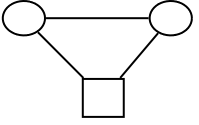
\includegraphics[scale=0.2]{images/21_Sim.png} <- explication d'une similitude \\
	- personnes \\
	- points d'intérêts 
\end{itemize}

\textbf{Idée générale}

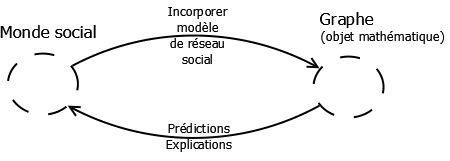
\includegraphics[scale=0.4]{images/21_IdeeGenerale.png}

\subsection{Exemples}
Il y a trois formes de fermeture
\begin{enumerate}
\item Fermeture triadique 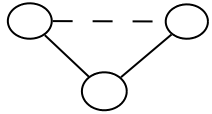
\includegraphics[scale=0.1]{images/21_FermetureTriadique.png}
\item Fermeture focale 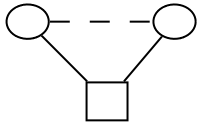
\includegraphics[scale=0.1]{images/21_FermetureFocale.png}
\item Fermeture d'adhésion 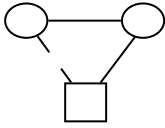
\includegraphics[scale=0.1]{images/21_FermetureAdhesion.png}
\end{enumerate}

\section{La formation des liens (selon les 3 approches)}
\begin{itemize}
\item On a des données réelles -> réseaux sociaux \\
		On a plus facilement un accès direct au graphes qu'avant.
\item mesurer empiriquement le taux de création des liens en fonction du nombres d'amis communs.
\end{itemize}

\subsection{Algorithme}
\begin{enumerate}
\item Capture à deux instants différents le réseau (appelons ces deux graphes (1) et (2))
\item Pour chaque entier "k" plus grand ou égal à 0 :
\begin{itemize}
	\item On identifie les paires de noeuds qui ont "k" amis en communs dans (1)
\end{itemize}
\item On regarde dans (2) si pour chaque paire un lien s'est formé
\end{enumerate}
=> On calcule T(k) = fraction des paires qui ont formé un lien

\subsection{Modèle pour expliquer ce résultat (fermeture triadique)}
Si on prend deux personnes : s'il y a 1 ami en commun, il y a une probabilité "p" qu'un lien se forme.\\
Quelle est la probabilité pour "k" amis en commun ?\\
=> On calcule la probabilité de "aucun lien se forme".

\paragraph*{}
La probabilité qu'aucun lien se forme quand il y a un ami en commun est de $(1-p)$.\\
On en déduit que pour "k" amis en commun, la probabilité est de $ (1-p)^{k}$\\
Dès lors, la probabilité qu'au moins 1 lien se forme pour k amis en commun est de $ 1-(1-p)^{k}$. C'est ce qui est égal à T(k).

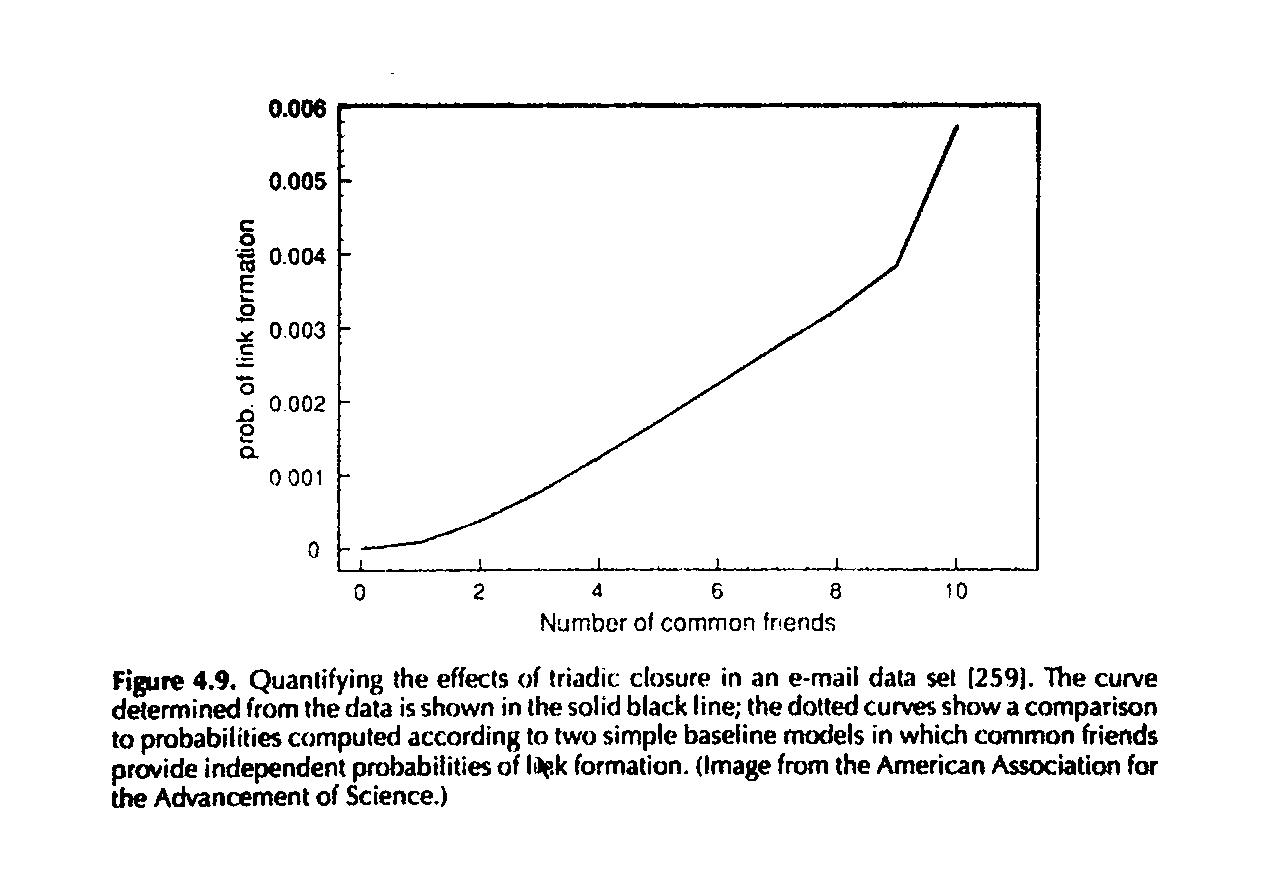
\includegraphics[width=\textwidth]{images/21_emailFriends.jpg}

On voit sur la figure 4.9 (fermeture triadique) que la probabilité qu'un lien se forme augmente exponentiellement avec le nombre d'amis en commun.

\paragraph{Attention !}
Le comportement et donc les calculs sont différents pour la fermeture focale et d'adhésion !

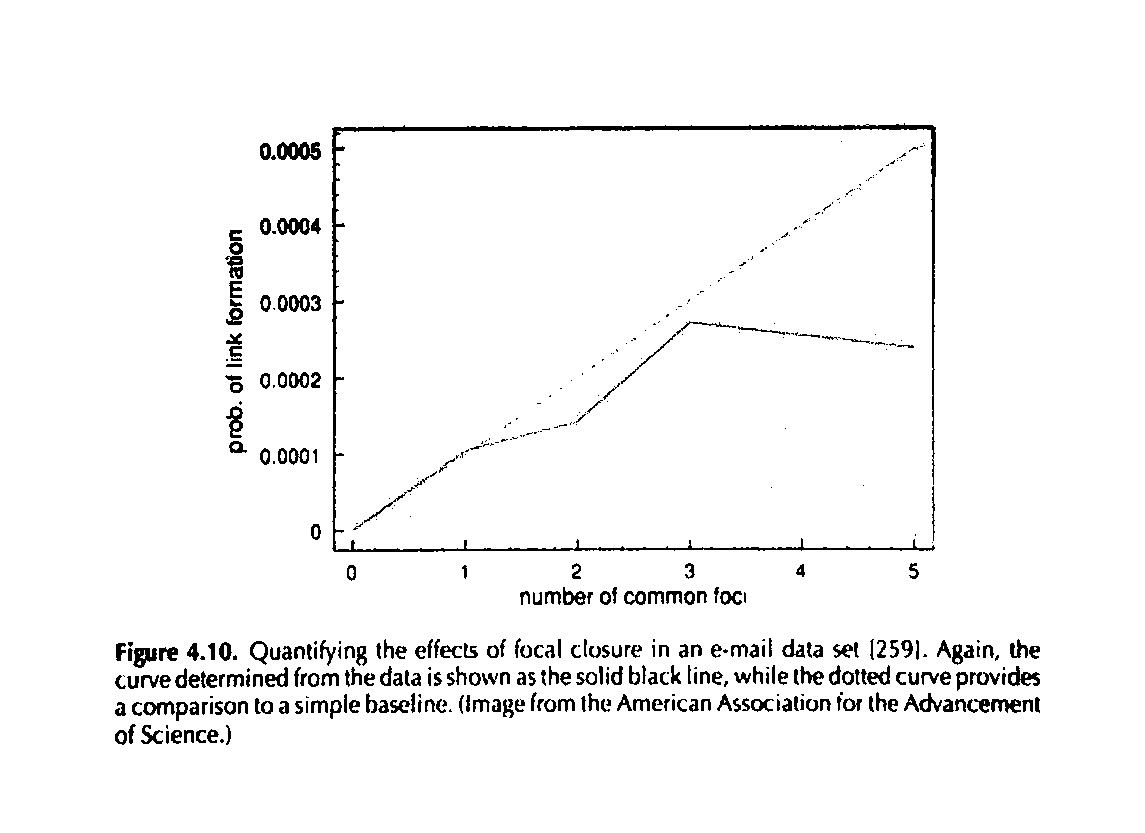
\includegraphics[width=\textwidth]{images/21_pointsCommuns.jpg}

La figure 4.10 (fermeture focale) nous montre que dans le cas où l'on considère le nombre d'intérêts en commun (ici, des cours), on arrive à un certains moment à saturation. Augmenter le nombre de points d'intérêts communs n'augmente plus la probabilité de création d'un lien à partir d'un certain point (ici 3 cours en communs).

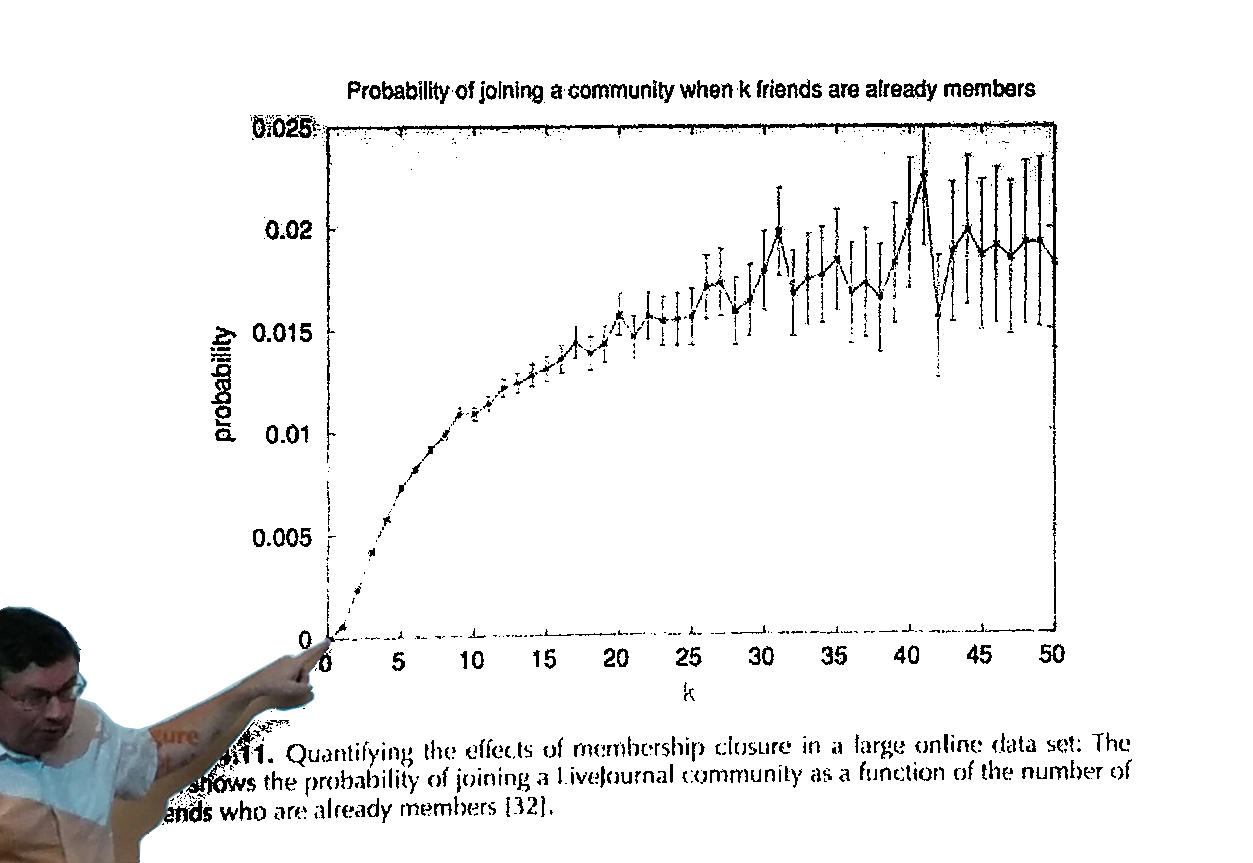
\includegraphics[width=\textwidth]{images/21_community.jpg}

Enfin, la figure 4.11 (fermeture d'adhésion) présente aussi un saturation à partir d'un certains nombre d'amis qui ont le même point d'intérêt.

\section{Quantifier les rôles relatifs de sélection d'influence sociale}
Les mécanismes de similitude :
\begin{itemize}
\item La sélection (intérieur, c'est nous qui faisons le choix)
\item L'influence sociale (extérieur, c'est les autres qui nous influencent) 
\end{itemize}
\subsection{Comment quantifier cela ?}
\paragraph*{Par exemple wikipédia}
Il peut exister une similitude de comportement entre rédacteurs. Par exemple les articles sur lesquels ils travaillent.\\
Raisonnement :
\begin{itemize}
\item On a des rédacteurs
\item Un lien entre deux rédacteurs : ils communiquent par la "Talk page" (chaque article a une "Talk page"). Autrement dit, si un rédacteur B communique sur la page de A, alors il y a un lien.
\item Les "points d'intérêts" ici sont les articles.
\item Quantification de la similitude = $\displaystyle\frac{\mbox{nombre d'articles rédigés par A ET B}}{\mbox{nombre d'articles rédigés par A OU B}}$\\
Notons dès lors que la similitude ne peut pas être plus petit que 0 ni plus grand que 1. $0 \leq sim \leq 1$
\item La rupture se fait quand le lien est créé. %schéma
\item On compare la similitude avant et après cette rupture (figure 4.13). C'est surtout la sélection qui joue avant, et l'influence sociale rentre en jeu après.
\end{itemize}

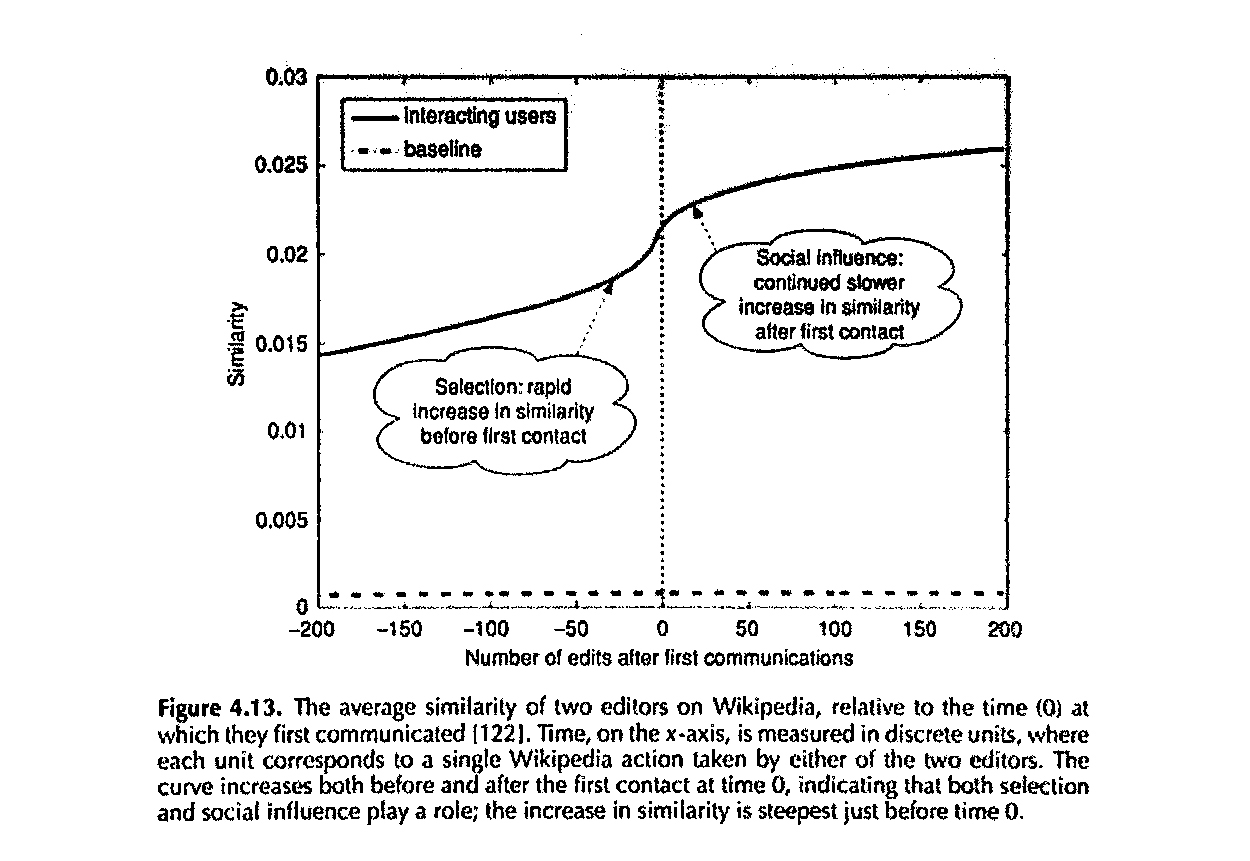
\includegraphics[width=\textwidth]{images/21_wikipedia.jpg}
  \section{Les relations positives et négatives}

Précédemment, les relations étudiées étaient considérées comme uniquement positives (on ne peut se faire que des amis). 

\includegraphics[scale=1]{images/22_force-positive}

Dans ce chapitre, nous allons étudier les graphes comportant également des relations positives et des relations négatives (on peut se faire des amis et des ennemis).

\includegraphics[scale=1]{images/22_amis-ennemis3.png}

\subsection{Théorie de l'équilibre de structure (Equilibre structurel fort)}
L'équilibre dans une structure va nous permettre d'identifier les situations stables et celles qui sont instables. Cette étude se fera dans un graphe complet (un graphe dont chaque paire a un lien et dont chaque lien peut être de type "+" ou "-").

\paragraph{}
L'idée cruciale est d'identifier dans le graphe les situations équilibrées et les situations qui ne le sont pas et qui engendrent un stress entre les nœuds.  

\begin{figure}[h!]
\label{equi}
\caption{Relations équilibrées et non équilibrées}
\centering
\includegraphics[width=\textwidth]{images/22_situation.png}
\end{figure}


Dans la figure \ref{equi}, les schémas de gauche sont considérés comme équilibrés. En effet, soit A, B et C sont tous amis et il n'y aucun conflit entre eux, soit B et C sont amis, mais sont en confit avec A. 
\paragraph{}
Par contre, les schémas de droite sont des situations non équilibrées. Dans la 3, B et C sont amis avec A mais ennemis entre eux, on peut supposer que A doive alors choisir un camp. La 4 indique que tous sont ennemis, mais il est fort probable que le graphe évolue vers une situation où deux nœuds se liguent contre le troisième. 

\paragraph{}
 
 On peut maintenant généraliser cela pour un nombre quelconque de nœuds. Ainsi un graphe complet sera équilibré si chaque ensemble de 3 nœuds est équilibré et donc possède des liens de type $+++$ ou $+--$.   

\begin{figure}[h!]
\label{equi2}
\caption{Généralisation des relations équilibrées et non équilibrées}
\centering
\includegraphics[width=0.5\textwidth]{images/22_situation2.png}
\end{figure}

\paragraph{}
Si un graphe n'est pas équilibré, il a tendance à s'équilibrer. 


\subsection{Caractérisation de l'équilibre structurel} 
Dans le point précédent, nous avons réalisé une définition avec des conditions locales, mais il est difficile de comprendre ce que cela fait pour tout le graphe.
Ainsi nous voudrions une définition globale (une caractérisation) sur l'ensemble du graphe.




\subsubsection*{Preuve:}
Pour prouver qu'un graphe est bien équilibré, il faut pouvoir démontrer dans les deux sens :
\begin{enumerate}

\item $\Rightarrow$ la structure est équilibrée 
$\rightarrow$ direction facile à déterminer
%% pas sur du tout!!!!!
\item $\Leftarrow$ équilibrée est la structure 
$\rightarrow$ direction plus complexe à déterminer

\end{enumerate}

\subsection{Théorème d'équilibre: [Frank Harary 1953]}
\begin{figure}[h!]
\label{groupami}
\caption{2 groupes d'amis qui sont ennemis entre eux.}
\centering
\includegraphics[width=0.5\textwidth]{images/22_amis-ennemies2.png}
\end{figure}

Si un graphe complet est équilibré, alors:

\begin{enumerate}

\item toutes les paires sont amies

\item on peut diviser les nœuds en deux groupes X et Y, tel que X et Y chacun contient des amis mutuels et chaque membre de X est ennemi de chaque membre de Y comme représenté à la figure : \ref{groupami}.

\end{enumerate}

\subsubsection*{Preuve:}

\begin{itemize}\renewcommand\labelitemi{\textbullet}

\item graphe complet, annoté $+,-$

\item graphe équilibré

\begin{enumerate}

\item si aucun lien négatif: (1)

\item sinon il existe un lien négatif

\end{enumerate}

\item prenons un nœud A quelconque

\item Définissons:

\begin{enumerate}

\item $X = A + $ tous ses amis
\item $Y = $ les ennemis de A

\end{enumerate}

\item Est-ce que X et Y satisfont la condition du théorème?
\end{itemize}

\subsubsection*{A démontrer:}


\begin{enumerate}

\item chaque paire dans X = amis

\item chaque paire dans Y = amis

\item chaque nœud de X est ennemi de chaque nœud de Y

\end{enumerate}


\includegraphics[scale=1]{images/22_amis-ennemies.png}

\subsubsection*{Exemple 1}

On peut retrouver ce type de comportement de graphe dans les relations internationales : lors de la séparation du Bangladesh au Pakistan en 1972, on a assisté à un surprenant soutien des États-Unis pour le Pakistan alors que celui-ci n'était pas un allié des Américains. 
\paragraph{Explication} 
Comme indiqué dans la figure \ref{paysconflit}, les USA désiraient se rapprocher de la Chine, pour y arriver, ils ont analysé les relations des différents pays de la région. Ils ont ainsi constaté que la Chine avait des ennemis communs avec le Pakistan. Un rapprochement avec le Pakistan lui permettait de rentrer dans le groupe des amis de la Chine.


\begin{figure}[h!]
\label{groupami}
\label{paysconflit}
\caption{Relation lors de l'indépendance du Bangladesh}
\centering
\includegraphics[scale=1]{images/22_pays-conflit.png}
\end{figure}
\paragraph{}
Une autre approche de ce conflit peut être réalisée d'un point de vue de la Chine : 
\begin{itemize}

\item Vietnam du Nord $\overset{+}{\longleftrightarrow}$ Inde

\item Pakistan $\overset{-}{\longleftrightarrow}$ pays du bloc EST

\item Chine : vote l'abolition du Bangladesh à l'ONU

\end{itemize}

\subsubsection*{Exemple 2}
Un autre exemple de ce jeu diplomatique est donné à la figure 55 du livre de référence et représente le jeu des alliances des grandes puissances européennes à la veille de la Première Guerre mondiale. 
\paragraph{}
 On assiste à un équilibrage du graphe des relations avec des pays qui changent continuellement d'alliés jusqu'au moment de la triple entente et de la triple alliance qui sépara tous les pays d'Europe en deux camps ennemis.

\subsubsection*{Exemple 3}
Dans ce troisième exemple, on touche directement les réseaux sociaux tel que Facebook et Twitter où il existe des relations \textit{Like ou Trust} et \textit{Dislike ou Distrust} dont les utilisateurs peuvent se servir pour juger le contenu des autres.
\paragraph{}
Le classement de produits y est libre: un utilisateur est libre d'avoir des opinions positives (+) ou négatives (-) sur les autres


\includegraphics[scale=1]{images/22_graphe-oriente.png}

\subsubsection*{Transitivité}  

Il est intéressant de savoir si les relations sont transitives ou non, autrement dit si A croit en B et que B croit en C, A croira-t-il en C?
\begin{align*}
A \overset{trust}{\longrightarrow} B \overset{trust}{\longrightarrow} C \overset{?}{\longrightarrow} A \overset{trust}{\longrightarrow} C
\end{align*}

Ou alors, si A n'a pas confiance en B et que B n'a pas confiance en C, est-ce que A aura alors confiance en C ou non?


\begin{align*}
A \overset{distrust}{\longrightarrow} B \overset{distrust}{\longrightarrow} C \overset{?}{\longrightarrow} &A \overset{trust}{\longrightarrow} C\\
&A \overset{distrust}{\longrightarrow} C
\end{align*}

Finalement, tout est possible selon le cas rencontré : 
\begin{itemize}
\item Si le trust signifie une relation d'amitié, la transitivité sera respectée. 
\item Si le trust indique une confiance sur l’opinion, la transitivité ne peut être respectée. 
\item Si par contre trust en une proximité dans les opinions politiques, un rapprochement de A et C est probable. 
\end{itemize}


\paragraph{Conclusion :}La théorie de l'équilibre structurel sera gérée selon le cas




\subsection{Équilibre structurel faible}
L'équilibre structurel faible, à l'instar de l'équilibre structurel fort, se base sur la
notion de stabilité des triangles du graphe. Mais contrairement à l'équilibre fort, on ajoute deux cas instables   

\includegraphics[scale=1]{images/22_Instabilite.png}

Un graphe complet annoté est faiblement équilibré si:
\begin{itemize}
\item aucun triplet n'est $++-$;
\item tous les triplets sont de type $+++, +--, ---$. 
\end{itemize}
\paragraph{}
L'équilibre faible permet une structure \textbf{multipolaire}.

\begin{figure}[h!]
\label{fig:multipolaire}
\caption{Structure multipolaire}
\centering
\includegraphics[scale=1]{images/22_etoile-amis.png}
\end{figure}



\subsubsection*{Théorème d'équilibre pour l'équilibre faible}

Si graphe complet annoté est faiblement équilibré, alors on peut diviser ses nœuds en groupes :

\begin{itemize}


\item dans un groupe: amis

\item autre groupe: ennemis

\end{itemize}

\paragraph{Preuve : } \textit{(analogue à la preuve sur l'équilibre structurel)}


\begin{enumerate}

\item Nœud A + tous ses amis appartiennent au groupe X \\
$\to$ amis mutuels, car ($+++$).

\item A $+$ ses amis sont ennemis avec tous les autres.

\item Enlever A $+$ ses amis : nouveau graphe.\\
$\to$ raisonnement récursif

\end{enumerate}

  \chapter{Structure du Web} %chapitre 13


\section{Mémoire associative - Hypertexte}

Liens hypertextes : chaque élément a des liens vers et depuis d'autres éléments. Un contenu hypertexte est un contenu auquel il est fait référence dans un document.

\vspace{0.5cm}
Deux exemples de contenus hypertextes :

$
\left. 
%\text{
\parbox{0.5\linewidth}{
\begin{itemize}
\item \textbf{Graphe de citations} \\
		Précurseur du web : nœuds indépendants, liens strictement vers le passé
\item \textbf{Encyclopédie} \\
		Les articles renvoient vers d'autres articles \\ (Wikipédia)
\end{itemize}
}%}
\hspace{0.5cm} \right\}
$ Réseaux d'informations




\begin{figure}[!h]
	\centering
	\includegraphics[scale=0.75]{images/23_image1.png}
	\caption{Liens hypertexte vers des articles}
	\label{hypertexte}
\end{figure}

\textbf{Problème de cohérence}

\begin{itemize}
\item \underline{Web}: Cohérence \textit{"a posteriori"} 
						\vspace{0.1cm}
                       \\ Le web n'ayant pas d'organisation, on va devoir en trouver une : un index ou un moteur de recherche
                       \vspace{0.2cm}
      
\item \underline{Wikipedia}: Cohérence \textit{"a priori"}
							\vspace{0.1cm}
                             \\ Une structure existe déjà, définie par les rédacteurs, les modérateurs et les règles de structure.
\end{itemize}

Le succès du Web réside dans la possibilité de trouver une structure \textit{a posteriori} à ce dernier, notamment grâce à l'algorithme PageRank. Altavista, Google, Lycos, ... proposent tous leur version de moteur de recherche. C'est grâce à l'efficacité de PageRank que Google s'est imposé largement comme moteur de recherche dominant.

\section{Le Web est un graphe orienté}
\begin{itemize}
\item \underline{Chemin dans un graphe orienté}: A $- \rightarrow$ B
\vspace{0.1cm}
\\Séquence de nœuds qui commence avec A et termine avec B et où chaque paire consécutive correspond à un lien orienté.

\item \underline{Connectivité}: 
\vspace{0.1cm}
\\Un graphe orienté est connexe s'il existe un chemin orienté entre chaque paire de nœuds.
\end{itemize}

\section{Composant fortement connexe (CFC) \\ \textit{Strongly Connected Component (SCC)} }

À l'intérieur d'un graphe orienté, un composant fortement connexe est :
\begin{itemize}
    \item Un ensemble de nœuds tel qu'il existe un chemin orienté entre chaque paire.
    \item L'ensemble ne fait pas partie d'un plus grand environnement ayant la même propriété. 
\end{itemize}

\begin{figure}[!ht]
\centering
\includegraphics[scale=0.3]{images/23_fig13-6.png}
% FIXME ce graphe a une faute : le SCC en bas à droite n'est pas vraiment un SCC, il y a un noeud qui ne convient pas.
\caption{Un graphe dirigé avec ses CFCs identifiés}
\label{cfc_exemple}
\end{figure}

Les CFCs forment un genre de \textit{"super noeud"}. Pour la connectivité, on peut ignorer la structure interne des CFCs.

\vspace{0.3cm}

On peut donc transformer le graphe en un graphe réduit : le CFC devient un unique nœud. Pour trouver qu'un chemin existe dans le graphe original, il suffit de trouver un chemin dans le graphe réduit.
Un exemple de transformation de ce type est illustré sur la figure \ref{cfc_transformation}.
\vspace{0.3cm}

\begin{figure}[!ht]
\centering
\includegraphics[width=0.85\linewidth]{images/23_schema2.png}
\caption{Exemple de transformation du graphe}
\label{cfc_transformation}
\end{figure}


\section{Web en nœud papillon (\textit{$\approx$ années 2000})}
	Maintenant, à quoi ressemble le graphe réduit du web ? Autour des années 2000, sa structure était proche de celle d'un nœud papillon, tel que celui représenté sur la figure \ref{noeud_papillon}.
	
	On repère trois composants principaux :
	\begin{itemize}
	\item Un composant "in", qui contient des liens hypertextes sortants.
	\item Un composant fortement connecté principal, qui forme un "noyau".
	\item Un composant "out", qui contient beaucoup de liens hypertextes entrants.
	\end{itemize}
	
	\begin{figure}[!ht]
		\centering
		\includegraphics[scale=0.25]{images/23_fig13-7.png}
		\caption{Structure en nœud papillon du web}
		\label{noeud_papillon}
	\end{figure}

\section{Émergence du Web 2.0 (\textit{$\ge$ années 2000})}
L'émergence du Web 2.0 se déroule entre 2000 et 2010. Il s'agit en fait d'un changement d'attitude général des certains acteurs importants du web conduisant à une structuration de la toile basée sur trois grands principes. 
\begin{enumerate}
    \item \underline{Création collaborative} de contenu plutôt que des pages personnelles.
    \item \underline{Services} vers lesquels sont transférés les données personnelles. Au lieu de publier du contenu  sur des sites personnels, les gens se tournent vers des services pour publier leur contenu (par exemple YouTube, Flicker, Github...)
    \item \underline{Personnes} au lieu des documents. On n'identifie plus un document en fonction de son contenu, mais en fonction de son auteur ou de la personne qui en est le sujet.
\end{enumerate} 

\vspace{0.3cm}
%\begin{minipage}{15cm}
\textbf{Technologies utilisées:}
    \begin{itemize}
        \item Blogs (Skyblog), ensuite détrônés par les réseaux sociaux (Facebook, Twitter, MySpace, Friendster...)
        \item Deep Web : création de page à la demande (créer un nouveau profil, une page Wikipédia, un groupe d'intérêt...)
        \item Cloud : regroupement et partage de ressources "à la demande", permet plus d'élasticité (adaptation en fonction des besoins)
    \end{itemize}
%\end{minipage}

\vspace{0.5cm}       

\newpage

%\hline 
\vspace{0.5cm}
    \textbf{Un petit bout d'histoire}
    
    \vspace{0.3cm}
    
    \underline{Quelques précurseurs} :
    
    \begin{itemize}
        \item \underline{1945 - Vannevar Bush} : Conseiller du président des États-Unis, Roosevelt\\ 
        Il a écrit un article intitulé "As We May Think" dans lequel il explique son appareil électronique relié à une bibliothèque et capable d'afficher des livres et de projeter des films appelé "Memex".
        \item \underline{1934 - Paul Otlet} : Documentaliste\\ 
        Il avait imaginé un système où l'on pourrait faire des recherches et consulter le résultat de ces recherches sur un écran. Cette intuition d'un pré internet est à l'origine d'une structuration des ressources des bibliothèques. Il est aussi un pionnier des microfiches, des fiches indépendantes qui stockent des informations, ayant une ressemblance non négligeable avec les pages web d'aujourd'hui.
        \item \underline{1990 - Tim Berners-Lee et  Robert Cailliau - CERN} : Inventeur du World Wide Web\\
        Ils se sont inspirés des écrits de Vannevar Bush pour inventer le WWW, avec sa structure de pages indépendantes reliées par des liens hypertextes.
    \end{itemize}
    
\vspace{0.5cm}


\chapter{Recherche dans le Web} %chapitre 14
Comment trouver une information ?
\vspace{0.3cm}

\underline{1960} : Concept de mot-clé $\rightarrow$ Limitations fortes

\begin{itemize}
    \item Limitations dues au concept de mot
        \begin{itemize}
            \item Synonymie : plusieurs mots pour le même concept.
            \item Polysémie : un mot pour plusieurs concepts.\\
            Par exemple les noms propres peuvent référer à plusieurs personnes, des lieux et des organisations.

        \end{itemize}
        
        Autrement dit, il n'y a pas de bijection entre les mots et les concepts.
        
    \item Limitations dues à l'abondance d'informations. \vspace*{0.2cm} \\
    $\left. %\text{
    \parbox{0.5\linewidth}{
        \begin{itemize}
            \item \underline{Avant}: Les informations sur le web étaient rares. 
            \item \underline{Maintenant}: Il y a beaucoup trop d'informations.
        \end{itemize}
        %}
        } \hspace{0.5cm} \right 
        \}
        $ Plus grand problème du web
\end{itemize}
    
	Pour résoudre le problème de surabondance d'informations, il faut trouver une façon de savoir quelle page est la meilleure. Comment faire ce choix ?
	
	La meilleure solution est d'utiliser l'information contenue dans la structure du réseau.
	
	
	
  \section{L'analyse des liens}
\begin{itemize}
\item Concentrateurs (\textit{Hubs})
\item Autorités (\textit{Authorities})
\item Comment trouver la meilleure page ? (Voir figure \ref{fig-14-1}	)
\end{itemize}



\begin{figure}[!h]
\centering
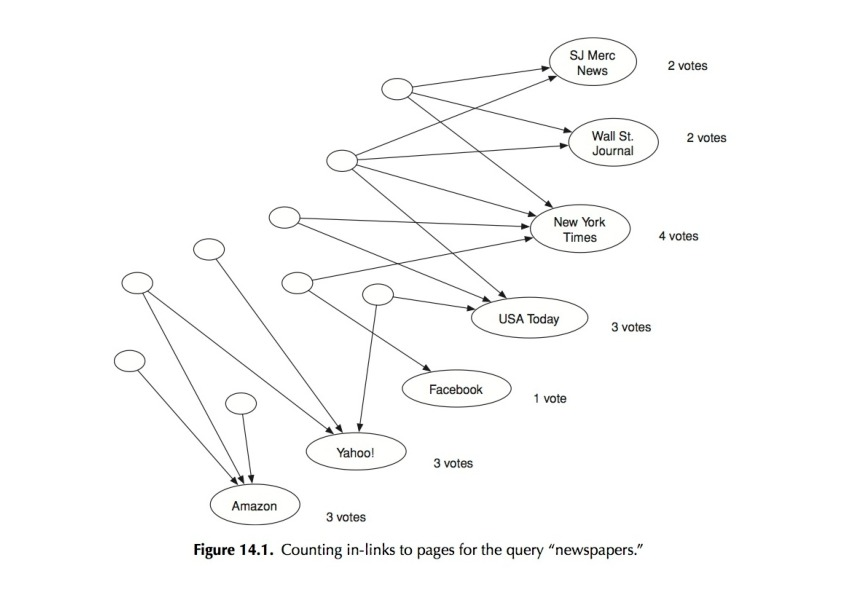
\includegraphics[scale=0.5]{images/ref/fig-14-1.jpeg}
\caption{Comptage des liens entrants pour la recherche "newspapers"}
\label{fig-14-1}
\end{figure}

\subsection*{Requête "newspapers"}

\paragraph{Pourquoi Facebook, Yahoo, Amazon, se retrouvent-ils dans la requette News Papers ?}
Car beaucoup d'utilisateurs ont des pages concentrées sur ces sites et comme dans cet exemple on utilise un algorithme qui n'est pas très sophistiqué, elles apparaissent. 

\paragraph{Comment trouver la meilleure page ?}
\begin{enumerate}
\item Compter les liens entrants comme une estimateur de la qualité d'une autorité.
\item Classer les concentrateurs en fonction de la qualité des pages qu'elles référencent.
\item Mettre à jour la qualité des autorités en fonction du poids de la source des liens.
\item Mettre à jour les concentrateurs.
\end{enumerate}

\subsubsection{Algorithme}

\begin{itemize}
\item Pages autorité (liens entrants) $ \rightarrow $ auto (p)
\item Pages concentrateurs (liens sortants) $ \rightarrow $ conc (p)
\item Mises à jour des liens entrants:
\begin{align*}
 auto'(p) =   \sum_ {p'\rightarrow p}conc(p') &&
\text{\emph{avec $p'\rightarrow p $ les pages p' qui ont un lien vers P}}
\end{align*}

\item Mises à jour des liens sortants: 
\begin{align*}
conc'(p) = \sum_ {p\rightarrow p'}auto(p') &&
\text{\emph{avec $p \rightarrow p' $ les pages p' qui sont référencées par p}} 
\end{align*}

\end{itemize}



\subsubsection*{Itération}}

$$
\forall~p~in~pages :
\left \{
\begin{array}{l}
auto(p) = 1 \\
conc (p) = 1 

\end{array}
\right.
$$

 Mise à jour, normalisation :
 
 \begin{align*}
 auto'(p) = \frac{auto (p)}{\sum auto(p')}
 \end{align*}
 \begin{align*}
 conc' (p) = \frac{conc (p)}{\sum conc(p)}
 \end{align*}
 Cet algorithme converge


En appliquant maintenant cet algorithme, la requête "newspapers" nous donnerait les résultats suivants (\ref{pageRankNews1} et \ref{pageRankNews2}):


\begin{figure}
\centering
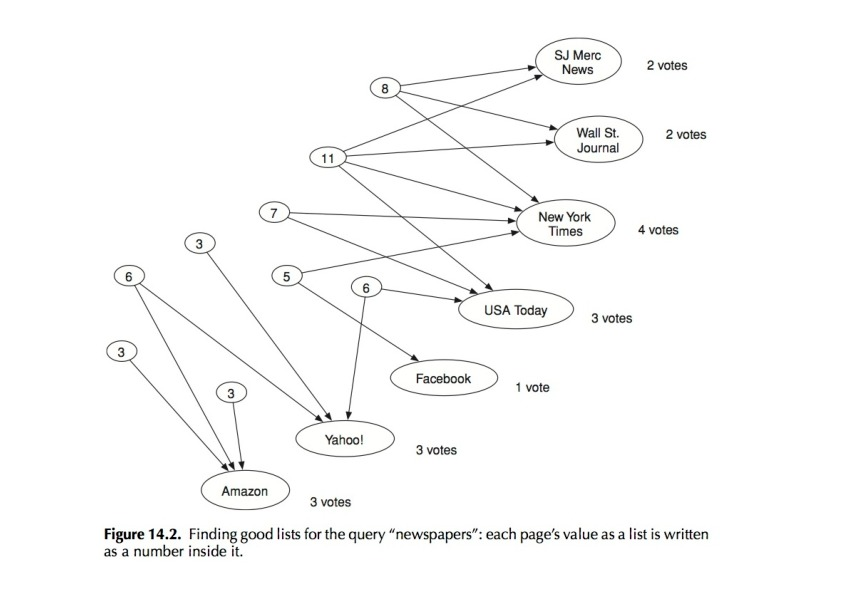
\includegraphics[scale=0.45]{images/ref/fig-14-2.jpeg}
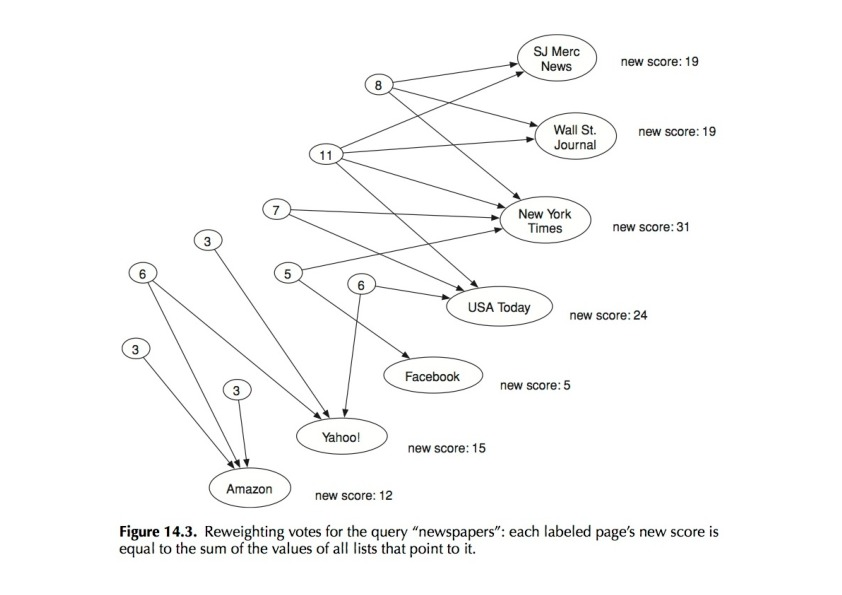
\includegraphics[scale=0.45]{images/ref/fig-14-3.jpeg}
\caption{Page Rank}
\label{pageRankNews1}
\end{figure}

\begin{figure}
\centering

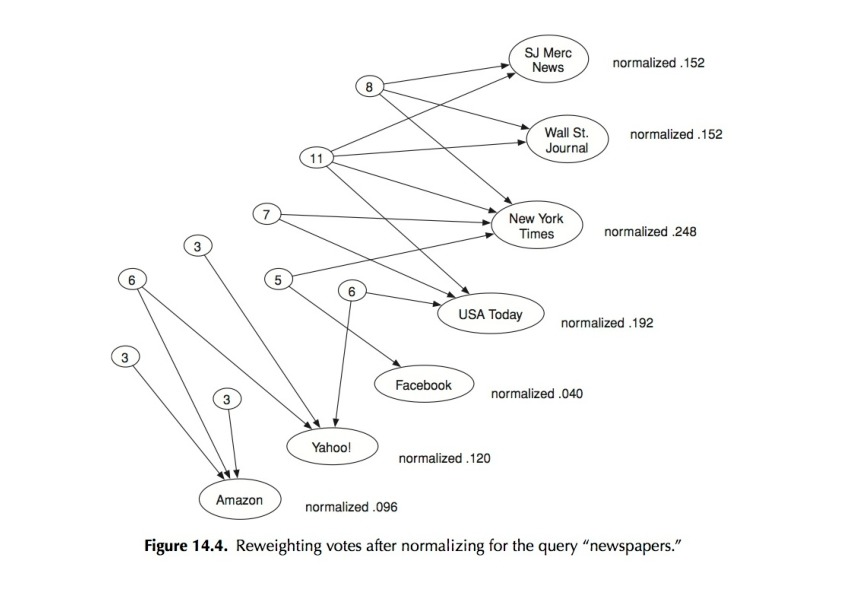
\includegraphics[scale=0.45]{images/ref/fig-14-4.jpeg}
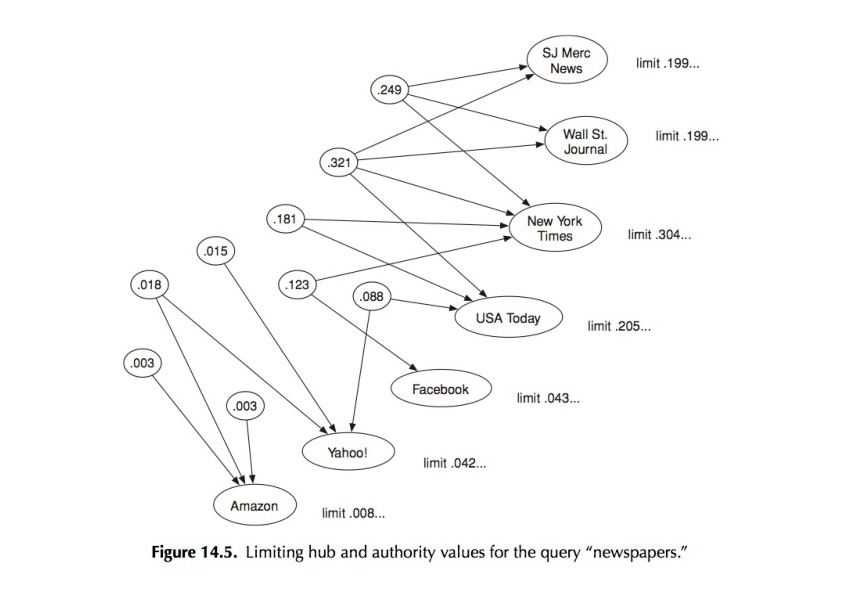
\includegraphics[scale=0.45]{images/ref/fig-14-5.jpeg}
\caption{Page Rank}
\label{pageRankNews2}
\end{figure}



\newpage

	
Comme nous pouvons voir, l'algorithme compte le nombre de liens entrants pour attribuer un poids à chaque place. Puis on normalise les valeurs trouvées, ce qui correspond au poids de la page.
Au plus grand est le poids d'une page au plus son autorité sera grande.

\section{PageRank}
\begin{itemize}
	\item Consolider autorités et concentrateurs.
	\item Une valeur par nœud : son "PageRank" que nous allons calculer. 
	\item Intuition: Un "fluide" qui circule dans le réseau. 
\end{itemize}

\textbf{ Algorithme PageRank :}
\begin{enumerate}
	\item N noeuds (chaque noeud représentant une page) :
	Initialisation Pr(p) =  $\frac{1}{n}$
	\item Choisir un nombre de pas k
	\item K mises à jour:\\
	Pr(p) = $ \sum_ {p'}\frac{Pr(p')}{n(p')} $ avec n(p') le nombre de liens sortant de p' et Pr(p') le poids (ou PageRank) de p' à la $k^{ème}$ itération.
\end{enumerate}
\subsection*{Exemple de PageRank :}

\begin{figure}[h!]
\centering
 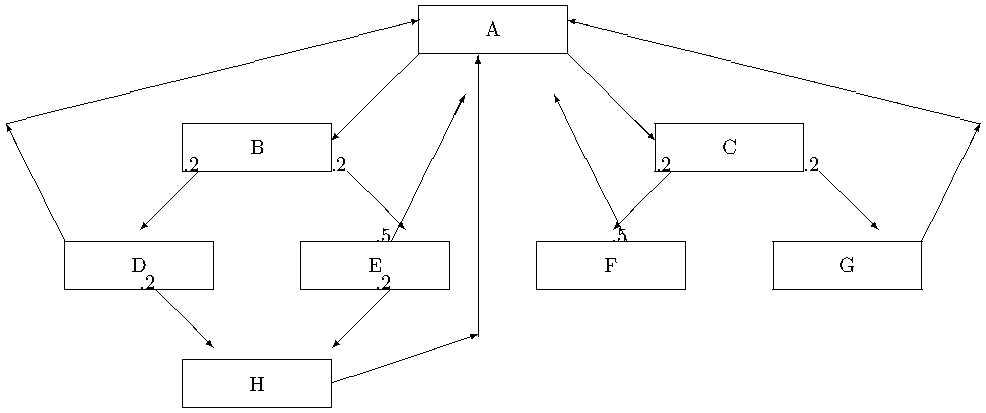
\includegraphics[scale=0.8]{images/24_imagePr.pdf}
\label{graphPageRank}
\end{figure}

 
 	\begin{tabular}{|c| c |c |c |}
		\hline
		Noeuds/Itérations & 0 & 1 & 2 \\
		\hline
		A & 1/8 & 1/2 & 5/16 \\
		B & 1/8 & 1/16 &  1/4   \\
		C & 1/8 & 1/16 & 1/4    \\
		D & 1/8 & 1/16 & 1/32  \\
		E & 1/8 & 1/16 &  1/32   \\
		F & 1/8 & 1/16 & 1/32    \\
		G & 1/8 & 1/16 & 1/32    \\
		H & 1/8 & 1/8 &  1/16   \\
		\hline
		$\sum $ & 1 & 1 & 1 \\
		\hline
	\end{tabular}


 Si nous continuons à laisser travailler l'algorithme, pour un nombre n fini d'itérations telles que k=n, il y aura convergence de l'algorithme. Dans cet exemple-ci,  nous aurons :

	$$Pr(A) = 4/13 ; Pr(B) = 2/13 ; Pr(C) = 2/13 ; Pr(Autres) = 1/13$$
 
Et la condition $\sum Pr(p) = 1$ est toujours vérifiée.
 
 L'équilibre est vérifié si le graphe est connexe,par contre si il ne l'est pas un problème se pose: Le fluide peut arriver au mauvais noeud (analogie réseau d'eau )  :

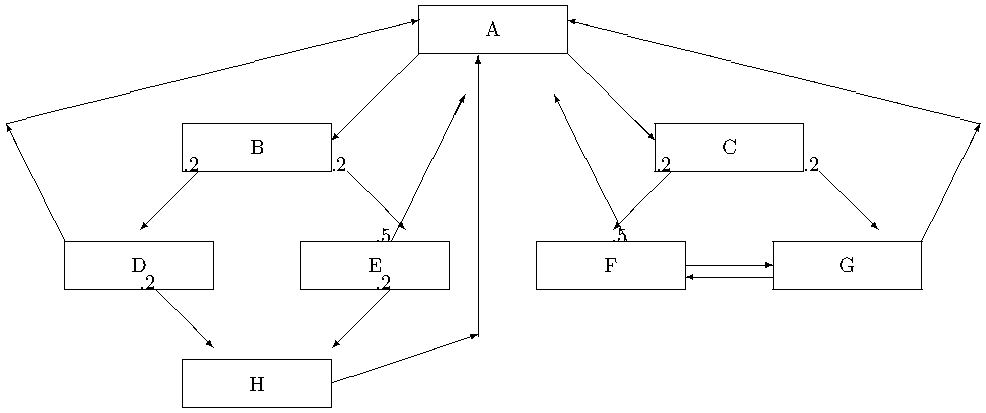
\includegraphics[scale=0.8]{images/24_Nconnexe.pdf}

\subsection*{Solution du problème}
	La solution dans le cas où le PageRank s'amasse dans un nœuds serait de former des cycles afin d'assurer que le fluide continue à circuler.
	
 	En pratique, on va réinjecter un peu de fluide partout à chaque itération pour éviter que le fluide se concentre dans les nœuds qui n'ont que des liens entrants et pas de liens sortant. De cette façon on referme la boucle et le fluide peut continuer à circuler.
 	
 	Cela peut s'apparenter à la circulation de l'eau dans l'atmosphère : le fluide s'évapore un peu partout et retombe de façon équitable.

	Ancienne règle de mise à jour :
	\begin{align*}
	Pr(p) =  \sum_ {p'}\frac{Pr(p')}{n(p')}
	\end{align*}
	
 	Nouvelle règle de mise à jour : \\
	\begin{align*}
         Pr(p) = S*Pr(p) + (1-S)  \times \frac{1}{n} \\
	 \text{Où S est un paramètre : $ 0 \le S \le 1 $} 
	\end{align*}
        
\subsection*{ Une autre manière de voir l'algorithme:}
    Cet algorithme correspond aussi au comportement des utilisateurs sur le web. La marche aléatoire d'un utilisateur sur le web peut être vue comme : 
	\begin{itemize}
        \item Probabilité de S : Suivre un lien dans la page web ou l'on se trouve.
        \item (1-S) : Choisir un n\oe ud au hasard, par exemple, taper une URL et accéder directement à un site.
        \item Pr(p), tel que calculé dans la nouvelle règle de PageRank, est la probabilité de tomber sur la page p.
	\end{itemize}
	
\subsection*{Historique de PageRank}

	PageRank a commencé à être utilisée au début des années 1990, mais a été en partie abandonné à partir de 2003-2004 pour bloquer les services de SEO (\textit{Search Engine Optimisation}) et autres manipulations du système comme les Google bombs\footnote{wikipedia.org/wiki/Google\_bomb}.
	
	Ceux-ci consistent à altérer les résultats de recherche soit en créant de nombreuses pages contenant des liens vers une page en particulier, soit en utilisant de gros concentrateurs qui contiennent énormément de mots-clés.
	
	Outre les modifications à l'algorithme de tri, certains sites utilisent aussi un attribut html "\textit{nofollow}" qui a pour effet que ces liens n'entrent pas en compte dans le PageRank d'une page. C'est notamment utilisé par les sites de blogging et les sites collaboratifs comme les wikis afin que personne n'ait intérêt à saboter une page pour ajouter un lien et améliorer le classement d'un site en particulier.\footnote{wikipedia.org/wiki/Nofollow}


  % \include{concl}
  % \newpage
  \phantomsection\addcontentsline{toc}{section}{Références}
\begin{thebibliography}{ABC}	
    \bibitem[Nis]{nis} Nimal Nissanke. \emph{Introductory Logic and Sets for Computer Scientists}.
    \bibitem[LPP]{eas} David Easley and Jon Kleinberg. \emph{Networks, Crowds, and Markets: Reasoning About a Highly Connected World}.
    \bibitem[Pro]{pro} Leon Sterling and Ehud Shapiro. \emph{The Art of Prolog}, MIT Press.
\end{thebibliography}

\end{document}

